\documentclass[10pt, conference]{IEEEtran}
\usepackage{graphicx}
\usepackage{amsmath}
\usepackage{amssymb}
\usepackage{booktabs}
\usepackage{tabularx}
\usepackage{caption}
\usepackage{subcaption}
\usepackage{tikz}
\usetikzlibrary{arrows.meta,positioning,fit,shapes.multipart}
\usepackage{cite}
\usepackage{xcolor}
\usepackage{array}
\usepackage{multirow}
\usepackage{enumitem}
\usepackage{balance}
\usepackage{needspace}
\usepackage[hidelinks]{hyperref}
\usepackage{placeins}
\usepackage{dblfloatfix}

% Tighter floats — reduces blank gaps and side-by-side table collisions
\setlength{\textfloatsep}{6pt plus 2pt minus 2pt}
\setlength{\floatsep}{6pt plus 2pt minus 2pt}
\setlength{\intextsep}{6pt plus 2pt minus 2pt}
\setlength{\dbltextfloatsep}{6pt plus 2pt minus 2pt}
\setcounter{topnumber}{5}
\setcounter{bottomnumber}{5}
\setcounter{totalnumber}{10}
\renewcommand{\topfraction}{0.92}
\renewcommand{\bottomfraction}{0.92}
\renewcommand{\textfraction}{0.08}
\renewcommand{\floatpagefraction}{0.75}

% Roman section numbering (per project brief)
\renewcommand{\thesection}{\Roman{section}}
\renewcommand{\thesubsection}{\thesection-\Alph{subsection}}

\title{Automatic Vehicle Gate Access System in All-Weather Conditions Using License Plate Recognition and Vehicle Make \& Model Recognition}

\author{\IEEEauthorblockN{Ali Raza Chaudhry and Abdul Hadi}
\IEEEauthorblockA{Department of Computer Engineering\\
COMSATS University Islamabad, Lahore Campus\\
Lahore, Pakistan\\
Supervisor: Dr.\ Taimoor Naeem\\
B.S.\ Computer Engineering}}

\begin{document}
\emergencystretch=2em
\graphicspath{{figures/}{figures/lpd/}{figures/pre/}{figures/lpr_char/}{figures/vmmr/}{figures/hw/}{figures/dashboard/}{final yolo/runs_backup/detect/predict/}}
\maketitle
\begin{abstract}
Outdoor vehicle gates must read license plates and verify vehicle identity under fog, rain, glare, and night exposure, yet many deployments still rely on plate-only decisions that are brittle to misreads and cloned plates. We present an integrated gate-recognition prototype that couples weather-aware preprocessing with a two-stage YOLOv8n license plate pipeline and an EfficientNet-B4 vehicle make and model recognizer (VMMR) over 245 classes, fused through a dual-check access policy in a web dashboard. Fog and haze are mitigated with a dark-channel prior and guided filtering; rain streaks are suppressed with oriented median filtering and Telea inpainting while protecting plate edges. On held-out benchmarks, YOLOv8n plate detection at epoch~50 reaches mAP@0.5 of 0.9807 (precision 0.9850, recall 0.9553), EfficientNet-B4 VMMR reaches 0.9624 Top-1 accuracy on 17{,}254 test images, and the character detector reports mAP@0.5 of 0.977 at epoch~100 only under mirrored training validation---a limitation we flag explicitly in Section~\ref{sec:disc}. The stack demonstrates end-to-end qualitative behavior under fog, rain, and night branches with restoration feeding both LPR and VMMR.
\end{abstract}

\begin{IEEEkeywords}
Automatic number plate recognition, vehicle make and model recognition, EfficientNet, YOLO, dark channel prior, rain removal, transfer learning, access control, intelligent transportation systems.
\end{IEEEkeywords}

\section{Introduction}
\label{sec:intro}
\subsection{Background and Motivation}
Manual barrier checks are expensive and slow, so many campuses and compounds now lean on cameras and software. That shift is understandable: nothing touches the vehicle, old lanes can be upgraded, and logs can store a timestamp plus stills when something looks wrong. The catch is almost always the weather. Fog smears the scene, rain scribbles bright lines across glass and paint, and harsh sun can blow out the plate. When the image degrades, both localization and reading suffer, which is why we spent time on preprocessing before feeding YOLO.

\subsection{Problem Statement}
Let $I \in \mathbb{R}^{H\times W \times 3}$ denote an RGB frame acquired at a gate lane. The system must estimate a plate string $s \in \Sigma^\ast$ over an alphabet $\Sigma$ and a fine-grained vehicle class $y \in \{1,\ldots,K\}$ (make-model family), then apply a decision rule $\mathcal{D}(s,y,\mathcal{W})$ conditioned on a whitelist $\mathcal{W}$ to produce an actuation command $a \in \{\textsc{grant},\textsc{deny},\textsc{alert}\}$. Informally, we want the same stack to work when $\omega$ labels fog, rain, or harsh glare, i.e., when the frame has been warped by a weather transform $T_\omega$. In practice that means either restoring $\hat{I}$ from $I$, accepting higher error, or collecting far more diverse training data than we had time for in an FYP semester.

\subsection{Research Gaps}
Industry ANPR kits are often sold on sunny-day demos, yet rain, fog, and night still move error rates in field reports~\cite{r05,r15}. Papers also tend to split the story: strong plate pipelines or strong make--model classifiers, but less documentation on how those pieces meet at a real gate with one camera stream and a latency budget~\cite{r08,r18}. Reviews of ITS deployments likewise describe ``plate reader here, classifier there'' integrations without much public detail on spoof resistance or audit trails~\cite{r01,r09}. We therefore document a single student codebase where defog/de-rain runs first, two YOLO stages read the plate, EfficientNet-B4 labels the car, and a small policy layer can disagree with a cloned plate scenario.

\subsection{Objectives, Contributions, and Scope}
We do not claim a new backbone; the contribution is wiring known blocks into one campus-style path. \textbf{Dual check:} whitelist on $s$ plus consistency against registered make/model from $y$. \textbf{Weather front-end:} fog and rain operators in Section~\ref{sec:pre} run before inference. \textbf{YOLO-centric LPR:} YOLOv8n for plate boxes and character boxes with regional formatting rules. \textbf{Reproducible metrics:} Section~\ref{sec:res} cites archived epoch checkpoints rather than rounded thesis headlines. Objectives follow the companion report: train plate and character YOLOv8n heads, classify 245 make--model families with EfficientNet-B4, encode dual-modality policy rules, and exercise fog, rain, and glare branches where data exists. ``All-weather'' here means fog/haze and rain branches in the integrated pipeline; snow, smog, and highway blur remain out of scope. Restoration runs before inference; the dual-check policy is coded for operator review though the relay is not wired---\textsc{alert} routes ambiguous cases to humans who still catch tailgating and behavioral cues cameras miss. Plate imagery raises indirect identification risks requiring signage, retention limits, and audit controls in production. For VMMR, ``accuracy'' means Top-1 unless noted; macro metrics weight every class equally. Every scalar in Section~\ref{sec:res} was transcribed from notebook outputs; character-stage validation mirrored training because Roboflow v4 shipped without a \texttt{valid} folder (Section~\ref{subsec:lpchar}).

\subsection{Paper Organization}
Section~\ref{sec:related} situates ANPR, VMMR, restoration, and embedded vision. Section~\ref{sec:theory} collects the math we lean on. Section~\ref{sec:system} sketches software and lane hardware. Sections~\ref{sec:data}--\ref{sec:vmmr} cover datasets, preprocessing, LPR, and VMMR. Section~\ref{sec:gate} states the policy; Section~\ref{sec:impl} lists tools and deployment cautions. Section~\ref{sec:res} presents figures and quantitative tables; Sections~\ref{sec:disc} and~\ref{sec:conc} interpret results and limitations. Appendices hold supplementary formulas and hardware specifications.

\section{Related Work}
\label{sec:related}

% --- Expanded related work (minimum 25 distinct works cited) ---
\subsection{ANPR and LPR Systems}
Classical ANPR chained edges, morphology, and template matching; it worked on clean plates but fell apart on blur, mud, or odd fonts. Convolutional features and deeper residual stacks made detection and reading far more robust. Single-shot detectors (SSD, YOLO families) trade a little box polish for speed that matters at a lane. Two-stage detectors such as Faster R-CNN still win when GPU budget is loose. Feature pyramids help with scale. We picked Ultralytics YOLOv8n simply because training, export, and Colab friendliness matched our timeline.

\subsection{Vehicle Make and Model Recognition}
Fine-grained classification means tiny visual gaps between classes. Big ``car in the wild'' datasets target boxes, not 245-way make/model folders. Everyone still initializes from ImageNet; EfficientNet-B4 gave us a accuracy--memory compromise we could train on a T4. We report macro metrics because head classes would otherwise drown the tail in a single accuracy number.

\subsection{Rain Streak Removal Techniques}
Rain priors often assume thin vertical structure. Learned derainers need paired data we did not curate, so we stayed with directional medians, bilateral smoothing, and Telea fills on small masks, while keeping plate edges out of the aggressive filters when possible.

\subsection{Low-Light and Night Image Enhancement}
Retinex-style and CLAHE-based tools are standard night fixes. Our LAB CLAHE stage is in the same family, even though the thesis narrative centers on fog and rain.

\subsection{Glare and Highlight Removal}
Hardware still wins here: polarizers, WDR modes, and exposure control. The Node dashboard optionally runs Sharp adjustments as a quick glare helper, not as a research-grade deraining substitute.

\subsection{Transfer Learning, Regularization, and Scaling Laws}
MixUp, CutMix, and Cutout are popular regularizers. We only used label-smoothed cross-entropy for VMMR to keep the training script short; the other tricks are noted as optional follow-ons.

\subsection{Embedded and Real-Time Vision Systems}
Older ITS work already argued about milliseconds per frame. Domain-shift surveys from medical imaging read surprisingly like security CV failures. Segmentation heads could help propose plates later; we did not add one in this milestone.

\subsection{Synthesis Relative to This Work}
Most papers stop at pretty restoration curves or at a single modality. We instead pipe restoration into YOLO, then into EfficientNet, and we spell out where resolutions disagree (224 versus 380) so the next student does not ``fix'' it silently.

\section{Theoretical Background}
\label{sec:theory}
\subsection{Convolutional Neural Networks}
A 2D convolution with kernel $K$ on feature map $X$ at location $(i,j)$ is
\begin{equation}
(K * X)_{i,j}=\sum_m\sum_n K_{m,n}\,X_{i+m,j+n}.
\label{eq:conv}
\end{equation}
ReLU activations $\phi(z)=\max(0,z)$ zero weak activations and keep gradients flowing. Pooling shrinks feature maps and buys tolerance to small shifts.

\subsection{Transfer Learning and Fine-Tuning}
Given a source task $S$ and target task $T$, transfer learning reuses representations $f_\theta$ learned on $S$ and adapts parameters on $T$. Fine-tuning updates all or a subset of layers; freezing early layers preserves generic edges/textures.

\subsection{EfficientNet and Compound Scaling}
EfficientNet scales depth $d$, width $w$, and resolution $r$ with compound coefficients~\cite{r27}:
\begin{equation}
d=\alpha^\phi,\quad w=\beta^\phi,\quad r=\gamma^\phi,\quad \alpha\beta^2\gamma^2\approx 2.
\label{eq:compound}
\end{equation}
MBConv blocks invert bottlenecks with depthwise separable convolutions and squeeze-excitation gating.

\subsection{CLAHE Theory}
CLAHE limits contrast amplification using a clip limit $C$ to prevent noise amplification in homogeneous regions. Processing the L channel in LAB decouples luminance from chrominance, reducing hue shifts.

\subsection{Morphological Image Processing}
Erosion and dilation with structuring element $B$ are
\begin{equation}
(I \ominus B)(x)=\min_{b\in B}I(x+b),\quad (I \oplus B)(x)=\max_{b\in B}I(x-b).
\label{eq:morph}
\end{equation}
Top-hat $T(I)=I-(I\circ B)$ highlights small bright structures when $B$ matches their scale.

\subsection{Gamma Correction}
Gamma maps intensities as
\begin{equation}
I_{\text{out}} = 255\cdot (I_{\text{in}}/255)^{1/\gamma}.
\label{eq:gamma}
\end{equation}
Values $\gamma<1$ brighten mid-tones; $\gamma>1$ darken them.

\subsection{OCR Pipeline Theory}
Classic OCR chains segmentation, feature extraction, and sequence decoding. Detection-based OCR with CNNs predicts character boxes directly.

% --- Additional theoretical material (CNNs, restoration, OCR theory) ---
\subsection{Convolutional Feature Hierarchies}
Early conv layers act like edge and blob filters; deep layers assemble parts. That hierarchy is why a single CNN can both localize a plate and, in a second head, fire on strokes inside the crop.

\subsection{Label Smoothing Cross-Entropy}
For hard targets $q$ and logits $z$, softmax probabilities are $p_i=\exp(z_i)/\sum_j\exp(z_j)$. Label smoothing replaces the one-hot target with
\begin{equation}
q'=(1-\epsilon)\,q+\epsilon/K
\label{eq:labelsmooth}
\end{equation}
over $K$ classes, discouraging overconfident logits at $\epsilon{=}0.1$ in our training code.

\subsection{AdamW Dynamics}
AdamW decouples $\ell_2$ regularization from the adaptive moment update, which tends to stabilize fine-tuning compared with older SGD recipes without warmup.

\subsection{Atmospheric Scattering and the Dark Channel}
Under a single-scattering approximation, scene radiance obeys
\begin{equation}
I(x)=J(x)t(x)+A(1-t(x)),
\label{eq:scatter}
\end{equation}
where $J$ is scene color, $A$ is airlight, and $t$ is transmission. The dark channel prior observes that most local patches contain at least one low-intensity channel in haze-free outdoor imagery, enabling $t$ estimation and dehazing. Guided filtering refines $t$ at object boundaries.

\subsection{Structural Similarity as a Supplementary Metric}
SSIM compares luminance, contrast, and structure between restored and reference frames when ground truth exists. For gate imagery, reference-free no-reference metrics (NIQE, BRISQUE) could complement PSNR/SSIM in future benchmarking.

\subsection{OCR as Sequence Decoding}
Beyond independent character boxes, sequence models (CTC, attention) decode variable-length strings. Our character model predicts boxes explicitly; sequence language models over plate lexicons could be fused as a future refinement.

\section{System Overview}
\label{sec:system}
\subsection{Full System Pipeline}
Figure~\ref{fig:flow} summarizes the end-to-end architecture: a USB camera captures frames that pass through resize, normalization, and all-weather enhancement; parallel YOLOv8n LPD and character OCR pipelines reconstruct plate text while EfficientNet-B4 classifies make and model; an authorization engine evaluates registered vehicles, access rules, and time constraints to produce \textsc{allow}, \textsc{deny}, or \textsc{temporary} decisions; and results sync over Wi-Fi to the Vercel dashboard with annotated snapshots and event logs. Target end-to-end latency is $\leq$2\,s per vehicle on the Orange Pi~5 Pro edge node.

\begin{figure*}[!tb]
\centering
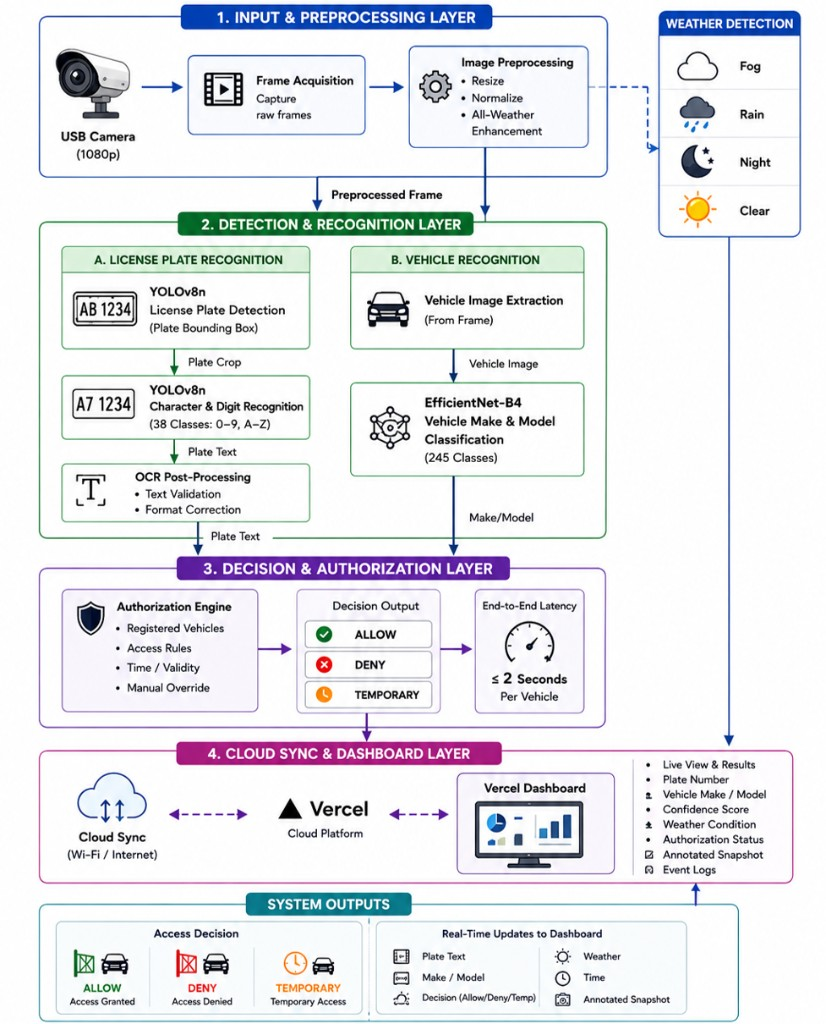
\includegraphics[width=\textwidth,keepaspectratio]{figures/system_overview_diagram.png}
\caption{System overview diagram. \textbf{Layer~1 (Input \& Preprocessing):} USB 1080p camera, frame acquisition, resize, normalize, and all-weather enhancement, with a side weather-detection module (fog, rain, night, clear). \textbf{Layer~2 (Detection \& Recognition):} YOLOv8n license plate detection, YOLOv8n character/digit recognition (38 classes) with OCR post-processing, and EfficientNet-B4 vehicle make/model classification (245 classes). \textbf{Layer~3 (Decision \& Authorization):} policy engine against registered vehicles, access rules, validity windows, and manual overrides. \textbf{Layer~4 (Cloud Sync \& Dashboard):} Wi-Fi sync to the Vercel platform for live view, confidence scores, weather, authorization status, and event logs.}
\label{fig:flow}
\end{figure*}

\subsection{Software Architecture}
Training lives in Colab notebooks (YOLOv8n LPD, YOLOv8n characters, EfficientNet-B4 VMMR). Runtime checkpoints are reused in the integrated pipeline and on the Orange Pi~5 Pro edge node, which also streams events to the Node/Express dashboard on Vercel. Datasets: Roboflow \emph{License Plate Project} v1 (CC BY~4.0) for plates; Roboflow \emph{My First Project} v4 for 38 glyph classes; and a 245-class VMMR corpus. Section~\ref{sec:pre} documents the fog/rain branches we batch through before plotting overlays.

\subsection{Web Dashboard}
\label{subsec:dashboard}
The React/Vite front end and Express API on Vercel form the management layer between edge inference and operators (Figure~\ref{fig:dashboard_arch}). Edge events are posted to the Vercel ingest endpoint; the server evaluates plate and make/model against the registered-vehicle database, persists events, and pushes live updates to the browser.

\textbf{Shared panels.} Both roles see a statistics dashboard (vehicle counts, authorized vs.\ unauthorized ratio, system status), a live feed with detection overlays and plate bounding boxes, and a weather monitor (temperature, humidity, visibility context for the preprocessing branch). JWT login enforces role-based access; the UI supports dark and light themes.

\textbf{Admin panel.} Administrators search vehicle logs (plate, model, confidence, weather, allow/deny outcome), issue manual gate open/close overrides, edit the authorized-vehicle database, grant or revoke elevated access, and tune detection thresholds, notifications, camera quality, and retention settings. Figure~\ref{fig:dashboard_admin} shows the admin \emph{Live Vehicle Feed}: sidebar links to Dashboard, Vehicle Logs, Manual Override, Admin Access Privileges, Settings, and Weather; the main pane streams edge-ingested frames with a green plate bounding box, status filters, auto-refresh, and session controls.

\textbf{User panel.} Standard operators monitor the live feed and weather views only. They may register temporary visitor vehicles via \emph{Refresh \& Add Vehicle} but cannot view full logs, override the gate, change system settings, or manage admin privileges. Figure~\ref{fig:dashboard_user} shows the reduced navigation (Live Feed, Weather, Add Temporary Visitor) and the same real-time detection window without administrative tools.

In operation the dashboard is \emph{secure} (JWT + RBAC), \emph{real-time} (instant ingest and UI refresh), \emph{all-weather ready} (weather tags travel with each event), and \emph{insightful} (annotated snapshots and decision cards for audit). Event-detail cards for authorized and denied vehicles appear in Figure~\ref{fig:hw_dashboard}.

\begin{figure*}[!tb]
\centering
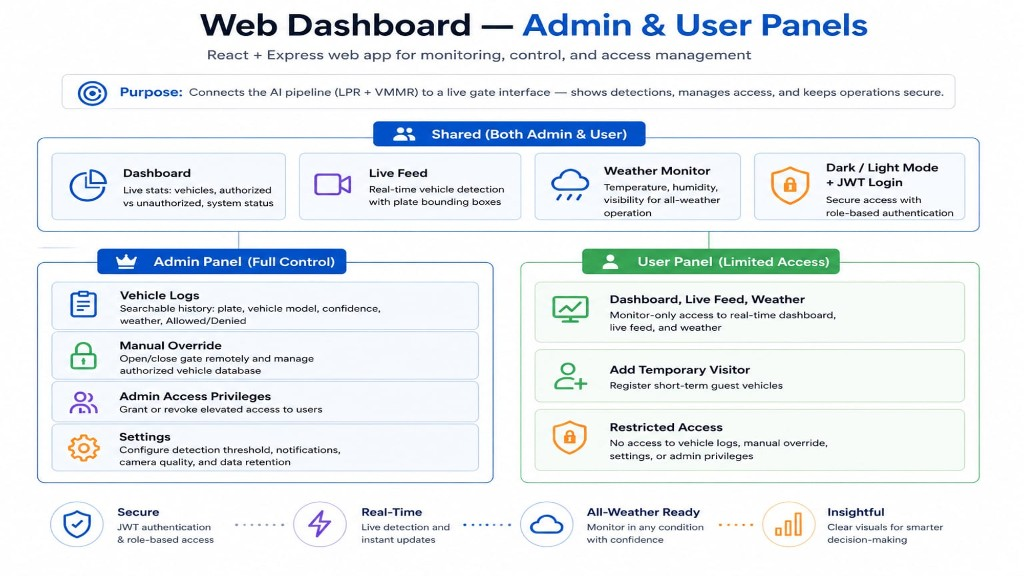
\includegraphics[width=\textwidth,keepaspectratio]{figures/web_dashboard_architecture.png}
\caption{Web dashboard architecture (React + Express on Vercel). \textbf{Shared:} statistics dashboard, live detection feed, weather monitor, JWT authentication, dark/light UI. \textbf{Admin:} searchable vehicle logs, manual gate override, database management, access control, and system settings. \textbf{User:} monitor-only access with temporary-visitor registration; no logs, override, settings, or admin tools.}
\label{fig:dashboard_arch}
\end{figure*}

\begin{figure*}[!tb]
\centering
\begin{subfigure}[b]{0.48\textwidth}
\centering
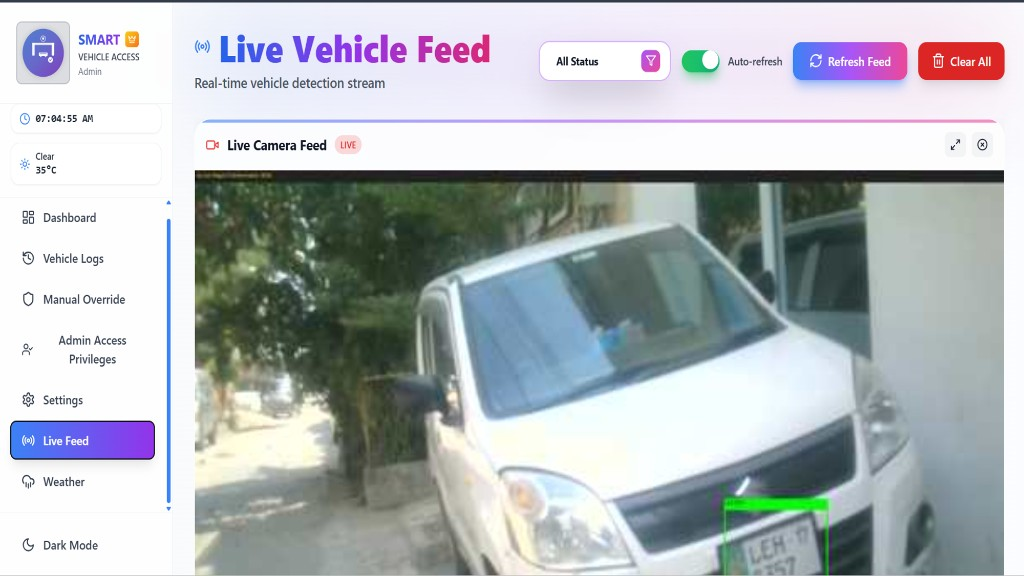
\includegraphics[width=\linewidth,keepaspectratio]{figures/dashboard/admin_live_feed.png}
\caption{Admin live feed with full sidebar (logs, override, privileges, settings).}
\label{fig:dashboard_admin}
\end{subfigure}\hfil
\begin{subfigure}[b]{0.48\textwidth}
\centering
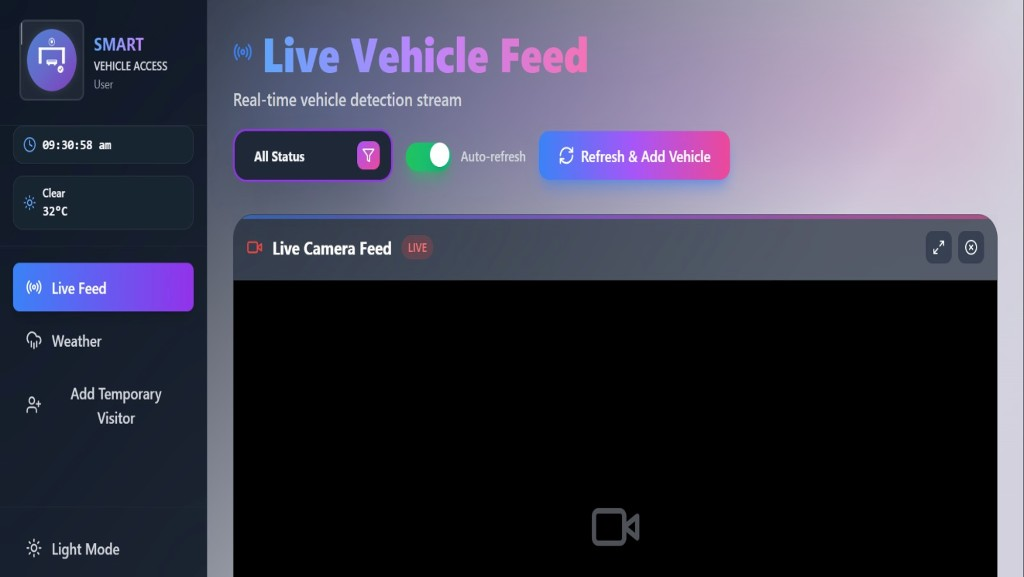
\includegraphics[width=\linewidth,keepaspectratio]{figures/dashboard/user_live_feed.png}
\caption{User live feed with monitor-only navigation and temporary-visitor entry.}
\label{fig:dashboard_user}
\end{subfigure}
\caption{Role-based dashboard UI (\emph{Smart Vehicle Access}). Both roles receive the live detection stream with plate overlays; JWT RBAC hides admin-only routes from standard users.}
\label{fig:dashboard_panels}
\end{figure*}

\subsection{Hardware Architecture}
Figure~\ref{fig:hw} shows the deployed edge hardware stack: a USB 1080p camera streams frames over USB to an Orange Pi~5 Pro (16\,GB), which runs YOLOv8n and EfficientNet-B4 inference locally; detection overlays, plate text, and vehicle labels are rendered on an HDMI monitor, while a 5\,V/5\,A supply powers the board. Thesis Appendix~C also lists future lane extensions---IR fill LEDs, relay-driven gate motor, outdoor enclosure, and weather sensors---summarized in Table~\ref{tab:hw} with status \emph{target} (T) versus lab-validated (L).

\begin{figure*}[!tb]
\centering
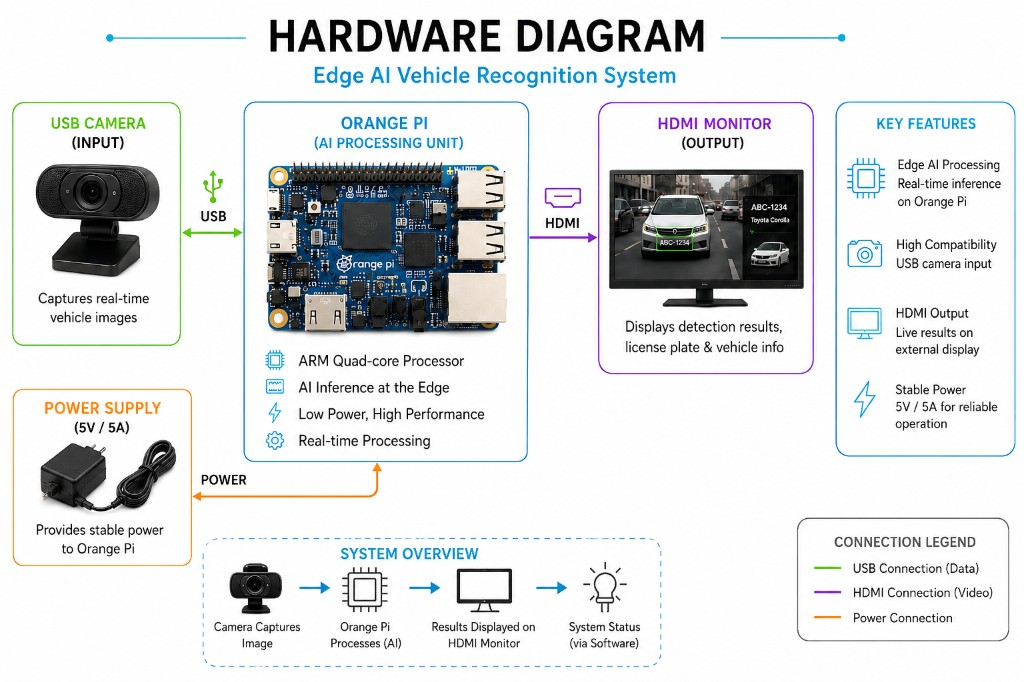
\includegraphics[width=\textwidth,keepaspectratio]{figures/hardware_diagram.png}
\caption{Hardware diagram of the edge AI vehicle recognition system. \textbf{Input:} USB camera captures real-time vehicle images. \textbf{Processing:} Orange Pi single-board computer (ARM quad-core, edge AI inference, low power) executes plate detection, character OCR, and VMMR classification. \textbf{Output:} HDMI monitor displays annotated detections, license plate text, and make/model labels. \textbf{Power:} regulated 5\,V/5\,A supply. Connection types: USB (data), HDMI (video), and dedicated power.}
\label{fig:hw}
\end{figure*}

\begin{table*}[!htbp]
\centering
\caption{Hardware components aligned with the thesis bill of materials (Appendix~C). Status: D=deployed and exercised, L=lab/software validation, T=target extension.}
\label{tab:hw}
\footnotesize
\begin{tabular}{@{}p{0.19\textwidth}p{0.28\textwidth}c p{0.40\textwidth}@{}}
\toprule
Component & Model / role & St. & Purpose \\
\midrule
IR camera + illuminator & Pole/lane imager, 850\,nm IR fill & T & Even plate visibility at night and in haze \\
Embedded computer & Orange Pi~5 Pro (16\,GB) & D & Edge inference, HDMI preview, Vercel sync \\
Validation workstation & CUDA-capable PC / Colab & L & Training and integrated notebook tests \\
Weather / light sensors & Rain, fog, lux probes & T & Future feedback to preprocessing branch \\
Gate motor & Sliding / swing mechanism & T & Physical lane barrier \\
Motor controller & Vendor gate drive (e.g., Centsys-class) & T & Safe motor commands from logic levels \\
Power supply unit & Regulated outdoor PSU & T & Stable power for camera, Pi, sensors \\
Relay module & Opto-isolated switching & T & Isolate Pi GPIO from motor loads \\
Enclosure \& glands & IP-rated cabinet & T & Environmental protection \\
Cabling & PoE or separate data + 12/24\,V runs & T & Power, Ethernet, sensor buses \\
\bottomrule
\end{tabular}
\end{table*}

\subsection{Edge Deployment Validation}
\label{subsec:hwdeploy}
The edge deployment stack loads the three trained checkpoints on the Orange Pi~5 Pro and processes USB-camera frames or batch image sets. Each inference cycle reports plate text, make/model label, weather branch, per-frame latency, and a gate-action token that is posted to the Vercel ingest API. Figures~\ref{fig:hw_batch}--\ref{fig:hw_dashboard} document representative runs.

\textbf{Batch and video inference.} Figure~\ref{fig:hw_batch} shows a 48-image rain folder processed without failures: plates such as \texttt{AT-990} and \texttt{PES-4321} are read, vehicles (e.g., Suzuki Mehran at 91.6\% confidence) are classified, and each event receives a dashboard ID with an \textsc{opened}/\textsc{closed} action. Figure~\ref{fig:hw_video} extends the same pipeline to video frames (e.g., frame~112 at 4.0\,s), stabilizing reads such as \texttt{LEH-8357} on a Suzuki Wagon~R across consecutive timestamps.

\textbf{Latency.} On-device timing stays within the $\leq$2\,s design target. Figure~\ref{fig:hw_latency} summarizes module ranges measured on the edge node: plate detection 80--200\,ms, character OCR 30--100\,ms, VMMR 200--800\,ms, and total pipeline 700--1000\,ms---consistent with the 725--846\,ms readings in the terminal logs.

\textbf{Local preview.} Figure~\ref{fig:hw_gui} pairs the OpenCV overlay window (\emph{FYP Gate Sync}) with console output for a handheld plate (\texttt{LEB-1481}, Toyota Yaris, 846\,ms), confirming that HDMI/local display and cloud sync run concurrently.

\textbf{Dashboard feedback.} Figure~\ref{fig:hw_dashboard} shows two ingested events on the live Vercel feed: (a)~a registered Suzuki Wagon~R (\texttt{LEH-8357}, 85.1\% confidence, gate \textsc{opened}); (b)~an unregistered Changan Alsvin (\texttt{BQX-687}, gate \textsc{closed}). Together these traces close the loop from edge capture through authorization to operator-visible audit records.

\begin{figure}[!t]
\centering
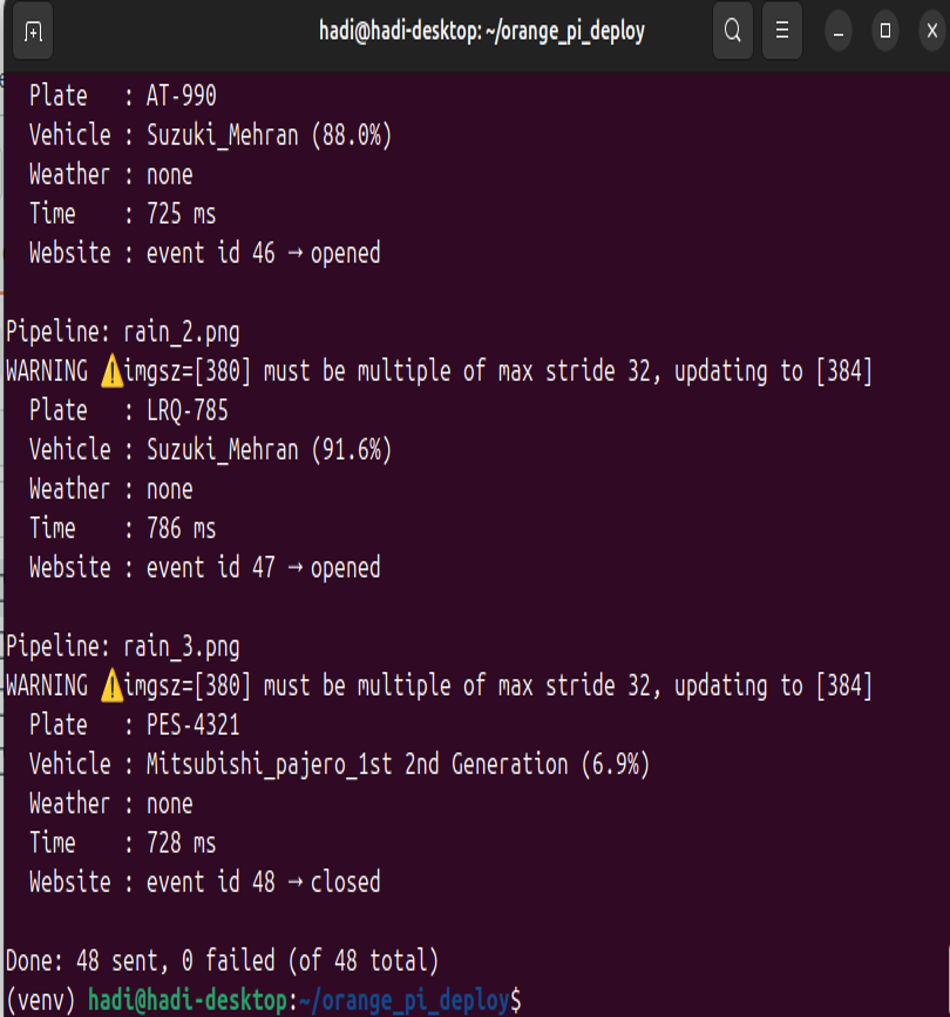
\includegraphics[width=\linewidth,keepaspectratio]{figures/hw/edge_batch_terminal.png}
\caption{Orange Pi batch run over 48 rain-scene images. Console fields: plate text, VMMR label with confidence, weather branch, frame time (ms), and Vercel event ID with gate action.}
\label{fig:hw_batch}
\end{figure}

\begin{figure}[!t]
\centering
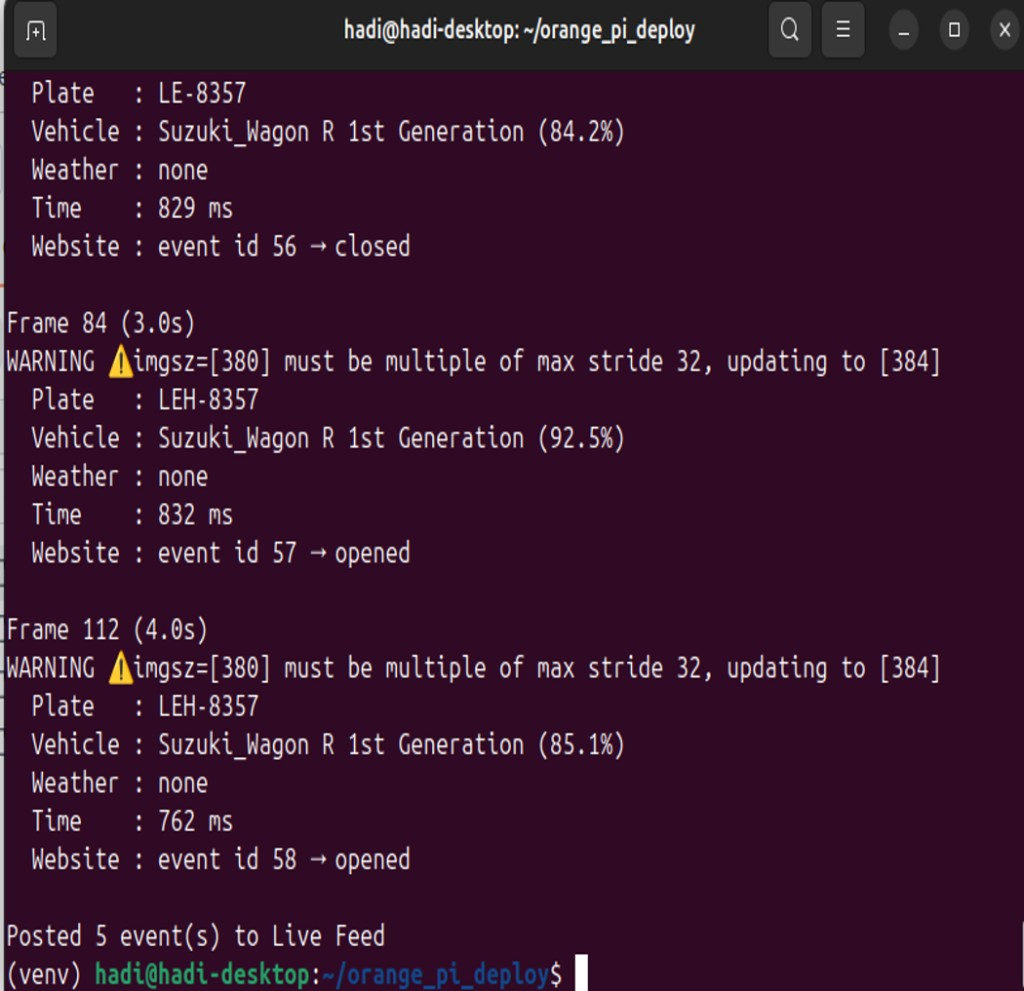
\includegraphics[width=\linewidth,keepaspectratio]{figures/hw/edge_video_terminal.png}
\caption{Video-frame inference on the edge node. Per-frame logs show plate stabilization (\texttt{LEH-8357}), vehicle identity, and sub-second latency before dashboard POST.}
\label{fig:hw_video}
\end{figure}

\begin{figure}[!t]
\centering
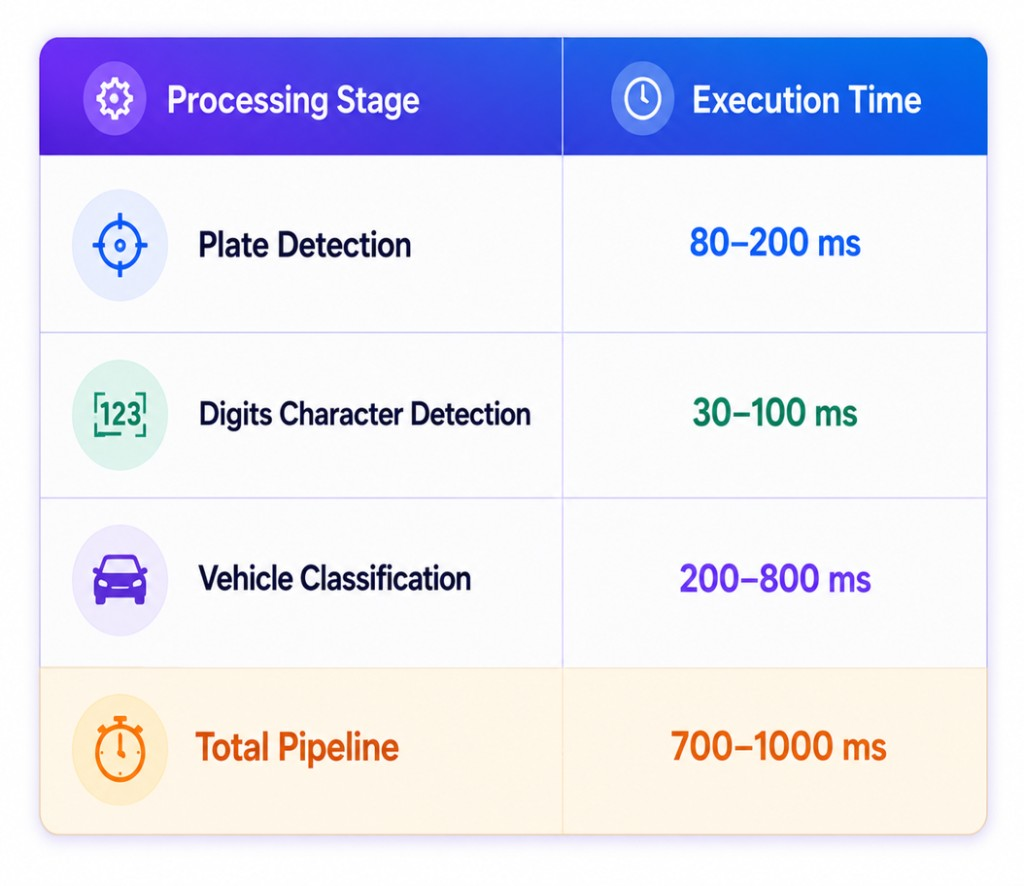
\includegraphics[width=0.92\linewidth,keepaspectratio]{figures/hw/edge_latency_table.png}
\caption{Per-stage execution time on Orange Pi~5 Pro. Character OCR is fastest; VMMR dominates total latency; end-to-end processing remains under one second in typical runs.}
\label{fig:hw_latency}
\end{figure}

\begin{figure}[!t]
\centering
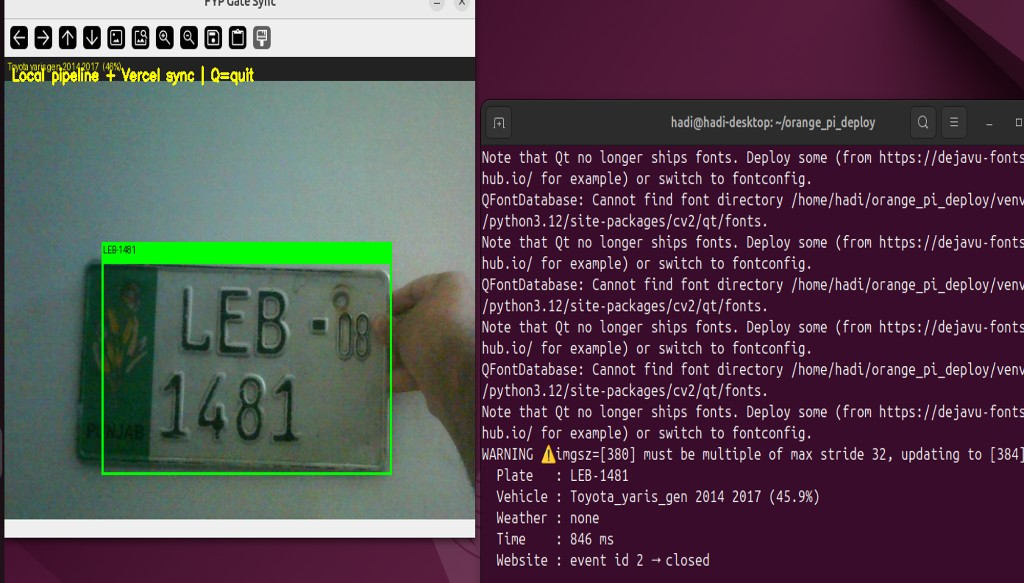
\includegraphics[width=\linewidth,keepaspectratio]{figures/hw/edge_live_gui.png}
\caption{Concurrent local GUI and terminal output during live capture. Green box marks the detected plate; yellow banner confirms Vercel sync; console reports 846\,ms end-to-end time.}
\label{fig:hw_gui}
\end{figure}

\begin{figure*}[!tb]
\centering
\begin{subfigure}[b]{0.48\textwidth}
\centering
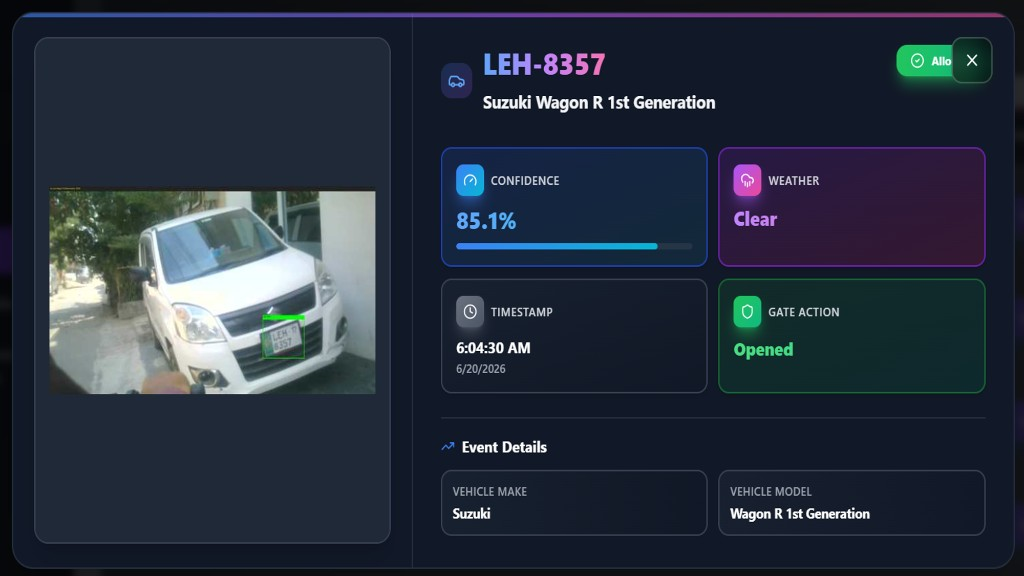
\includegraphics[width=\linewidth,keepaspectratio]{figures/hw/dashboard_allowed.png}
\caption{Registered vehicle: \textsc{allowed}, gate opened.}
\label{fig:hw_dash_allow}
\end{subfigure}\hfil
\begin{subfigure}[b]{0.48\textwidth}
\centering
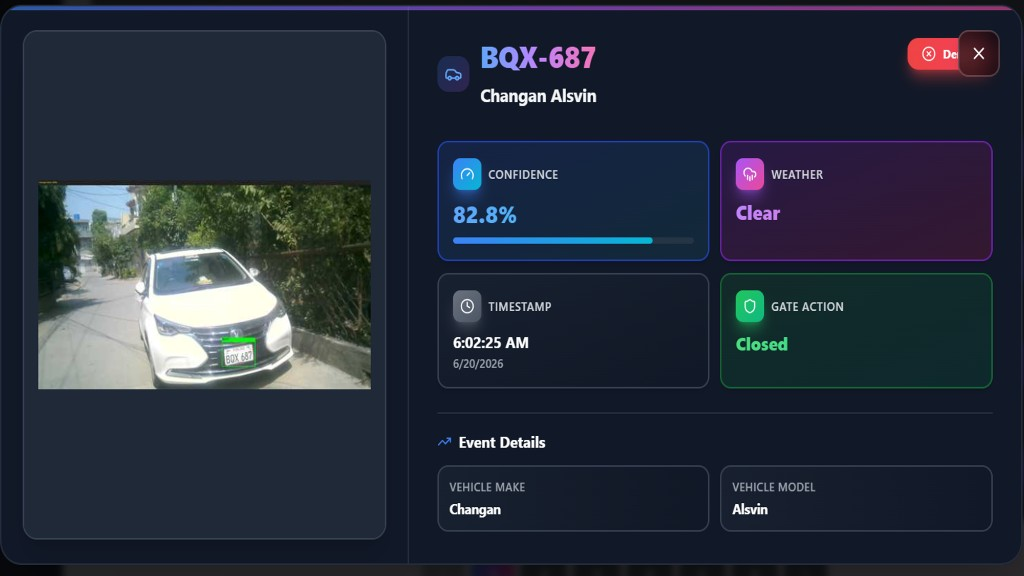
\includegraphics[width=\linewidth,keepaspectratio]{figures/hw/dashboard_denied.png}
\caption{Unknown vehicle: gate closed.}
\label{fig:hw_dash_deny}
\end{subfigure}
\caption{Vercel dashboard live feed after edge ingest. Left: authorized Suzuki Wagon~R (\texttt{LEH-8357}). Right: unregistered Changan Alsvin (\texttt{BQX-687}). Cards show confidence, weather, timestamp, and gate action.}
\label{fig:hw_dashboard}
\end{figure*}

\section{Dataset Description}
\label{sec:data}
Plate localization uses the Roboflow Universe export \emph{License Plate Project} v1: JPEG frames with YOLO labels and public splits (Section~\ref{sec:lpr}, Table~\ref{tab:splits}).

VMMR images sit in 245 make--model folders with train/test trees plus the 20\% validation split carved out inside the training folder (Section~\ref{sec:vmmr}). Characters come from Roboflow \emph{My First Project} v4 (1{,}235 crops, 38 classes). Figures and tables for all three sources land in Section~\ref{sec:res}.

\begin{table}[!htbp]
\centering
\caption{Dataset split summary (Roboflow exports for LPR; notebook counts for VMMR). Character training mirrors the training pool into validation (Section~\ref{subsec:lpchar}).}
\label{tab:splits}
\footnotesize
\begin{tabular}{@{}lrrrr@{}}
\toprule
Split & Train & Val & Test & Total \\
\midrule
LPD (Roboflow v1) & 20580 & 1973 & 978 & 23531 \\
LPR chars (\emph{My First Project} v4) & 1235 & 0 & 0 & 1235 \\
VMMR (245-class corpus) & 31904 & 7977 & 17254 & 57135 \\
\bottomrule
\end{tabular}
\end{table}

\section{Image Preprocessing Module}
\label{sec:pre}
\subsection{Scope and Integration}
Fog and rain preprocessing share the same runtime as the two YOLO heads and EfficientNet so we are not juggling mismatched configs when we screenshot results. Runtime loads three checkpoints: plate YOLO, 38-class YOLO, 245-way EfficientNet-B4. Fog/haze follows a dark-channel estimate, guided filter refinement, optional residual-haze mask, gray-world white balance, adaptive gamma, LAB CLAHE, a small saturation lift, bilateral polish, and a touch of unsharp. Rain builds an edge mask, runs three vertical median kernels (15/11/7) with a brightening guard, then Telea-inpaints tiny blobs. Night/low-light tiles reuse the same weights after a lighter tone curve; they sit beside fog and rain in Section~\ref{sec:res} (Subsection~\ref{subsec:prefigs}). Good camera WDR and IR fill still matter more than any slider (Section~\ref{sec:system}).

\subsection{End-to-End Inference Chain}
The demo resizes the vehicle crop to $380\times380$ for VMMR, runs plate YOLO at 0.25 confidence, pads each plate crop, runs character YOLO at 0.25, sorts glyph centers on $x$, and applies the ``up to three letters + up to four digits + hyphen when both exist'' formatter we coded for regional layouts.

\subsection{Demonstration Workflow}
We batch up to ten images per branch, show input versus restored pairs, then overlay boxes and text. A human picks fog versus rain today; there is no tiny weather CNN yet.

\subsection{Dashboard and Deployment Hooks}
The web client may run Sharp normalization before upload for harsh glare. Weather and authorization metadata are attached at ingest time (Subsection~\ref{subsec:dashboard}); automatic sensor-driven branch selection remains future work.

\begin{table}[!htbp]
\centering
\caption{Representative restoration and rain-removal hyperparameters.}
\label{tab:preparams}
\begin{tabular}{@{}ll@{}}
\toprule
Component & Setting \\
\midrule
Fog DCP patch / $\omega$ (primary) & $13\times13$ / 0.95 \\
Fog guided filter ($r$, $\varepsilon$) & 50, $10^{-3}$ \\
Fog residual mask & mean${>}170$, std${<}30$, Gaussian blur $21\times21$ \\
Fog CLAHE & clip limit 2.5, tiles $8\times8$ \\
Rain bilateral / Canny & (9,75,75) / (50,150) \\
Rain vertical medians & $k\in\{15,11,7\}$ \\
Rain brightening guard & discard if $\Delta$mean${>}2$ \\
Rain Telea inpaint & radius 3, spots area $\in(2,250)$ \\
\bottomrule
\end{tabular}
\end{table}

\section{License Plate Recognition Module}
\label{sec:lpr}
\subsection{Pipeline Overview}
LPR is deliberately two-stage: find the plate, then read glyphs inside the padded crop. Stage one uses Roboflow v1; stage two uses \emph{My First Project} v4 (Section~\ref{subsec:lpchar}). Figure~\ref{fig:modelarch} summarizes both recognition stacks: YOLOv8n plate detection at $380\times380$, character OCR at $640\times640$ over 38 classes, and EfficientNet-B4 VMMR at $224\times224$ over 245 make--model labels.

\begin{figure*}[!tb]
\centering
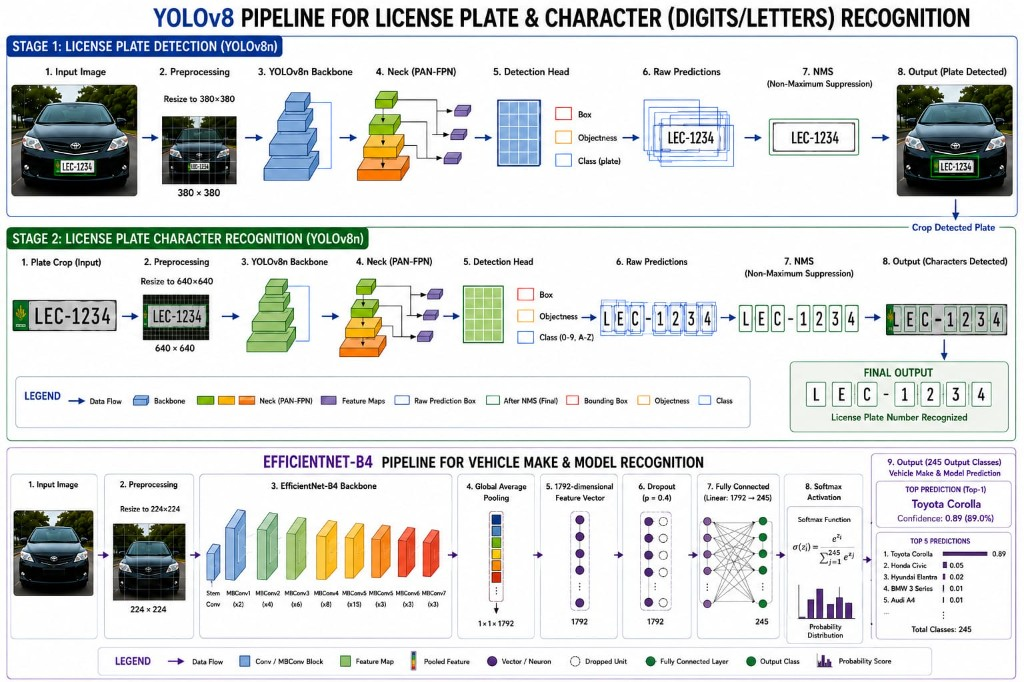
\includegraphics[width=\textwidth]{figures/model_architecture_diagram.png}
\caption{Recognition model architectures. \textbf{Top (YOLOv8n LPR):} Stage~1 resizes the vehicle frame to $380\times380$, runs backbone--neck--head detection, and applies NMS to obtain a plate crop; Stage~2 resizes the crop to $640\times640$, detects 38 character classes, and formats the read string (e.g., LEC-1234). \textbf{Bottom (EfficientNet-B4 VMMR):} $224\times224$ input passes through MBConv blocks, global average pooling, dropout ($p{=}0.4$), and a 245-way softmax head (example Top-1: Toyota Corolla, 89.0\%).}
\label{fig:modelarch}
\end{figure*}

\subsection{License Plate Detection (YOLOv8n LPD)}
Roboflow \emph{License Plate Project} v1 ships \textbf{20{,}580} train, \textbf{1{,}973} validation, and \textbf{978} test JPEGs (\textbf{23{,}531} total) with one plate class per label file. We trained YOLOv8n for 50 epochs, batch~32, requested 380-pixel squares; Ultralytics rounded to $384\times384$. Mixed precision stayed on with stock augmentations on a rented Tesla~T4. Table~\ref{tab:lpdtrain} is the run card; Table~\ref{tab:lpdmetrics} lists epoch~50 box metrics only (no character accuracy yet).

\begin{table}[!htbp]
\centering
\caption{LPD training configuration (archived run).}
\label{tab:lpdtrain}
\begin{tabular}{@{}ll@{}}
\toprule
Field & Value \\
\midrule
Architecture & YOLOv8n (nano, ImageNet-pretrained backbone) \\
Epochs / batch / request size & 50 / 32 / 380 (effective $384\times384$ train/val) \\
NMS train IoU & 0.7 (default) \\
Optimizer / AMP & automatic (MuSGD in log) / enabled \\
Run identifier & lp\_detector2 (auto-suffixed) \\
Runtime (logged) & Ultralytics 8.4.x, PyTorch 2.10+cu128, Tesla T4 \\
Splits & Roboflow train / valid / test \\
\bottomrule
\end{tabular}
\end{table}

\begin{table}[!htbp]
\centering
\caption{LPD validation metrics at epoch~50 (box localization).}
\label{tab:lpdmetrics}
\begin{tabular}{@{}lcccc@{}}
\toprule
Metric & P & R & mAP@0.5 & mAP@0.5:0.95 \\
\midrule
Value & 0.9850 & 0.9553 & 0.9807 & 0.7073 \\
\bottomrule
\end{tabular}
\end{table}

We also rendered some validation plots at $640\times640$ for readability; do not mix those curves with the $384$-anchored training log without retuning.

\subsection{Character and Digit Detection (YOLOv8n)}
\label{subsec:lpchar}
Stage two trains 100 epochs at $640\times640$ on \textbf{1{,}235} crops from Roboflow \emph{My First Project} v4 (CC BY~4.0) with 38 classes (digits, capitals, export quirks). The export contained only a training split; we mirrored it into validation so Ultralytics would not crash, which means Table~\ref{tab:lpcharmetrics} and Figure~\ref{fig:ocrmetrics} are optimistic. Roboflow stretched exports to $512\times512$ before we upsampled again inside Ultralytics.

\begin{table}[!htbp]
\centering
\caption{LPR character-stage training configuration.}
\label{tab:lpchartrain}
\begin{tabular}{@{}ll@{}}
\toprule
Field & Value \\
\midrule
Architecture & YOLOv8n (nano) \\
Epochs / batch / size & 100 / 16 / $640\times640$ \\
Dataset & Roboflow \emph{My First Project} v4 \\
Classes & 38 \\
Validation split note & No held-out exporter split; validation mirrors training \\
\bottomrule
\end{tabular}
\end{table}

\begin{table}[!htbp]
\centering
\caption{LPR character-stage validation summary at epoch~100 (mirrored validation pool; values match Figure~\ref{fig:ocrmetrics}).}
\label{tab:lpcharmetrics}
\begin{tabular}{@{}lc@{}}
\toprule
Metric & Value \\
\midrule
mAP@0.5 & 0.977 \\
Precision & 0.990 \\
Recall & 0.942 \\
F1 score & 0.965 \\
FPR & 0.010 \\
mAP@0.5:0.95 (Ultralytics export) & 0.7611 \\
\bottomrule
\end{tabular}
\end{table}

\subsection{Integrated Runtime Hooks}
The integrated pipeline loads the same LPD weights at 0.25 confidence, runs characters at 0.25, and maps detections through the 38-class label vocabulary.

\subsection{Formatting Heuristic}
We sort by $x$-center, keep up to three letters on the left and up to four digits on the right, and insert a hyphen when both groups exist so the string resembles local plates.

\subsection{End-to-End String Metrics}
Box metrics live in Tables~\ref{tab:lpdmetrics} and~\ref{tab:lpcharmetrics}. Full-string accuracy after fog/rain branches is deferred to future work (Section~\ref{sec:conc}); Section~\ref{sec:res} shows qualitative overlays meanwhile.

\section{VMMR Module}
\label{sec:vmmr}
\subsection{Architecture}
EfficientNet-B4 starts from ImageNet weights; we swap the classifier for a 245-unit linear layer and train with cuDNN benchmark mode on for fixed shapes. Checkpoints store class names plus optimizer state. Figure~\ref{fig:modelarch} shows the MBConv backbone, pooling head, and 245-way softmax output used at test time ($224\times224$).

\subsection{Dataset}
Images are organized in a standard class-folder layout with 245 vehicle labels. One corrupt image was skipped during a manual scan. After cleanup: \textbf{31{,}904} training images, \textbf{7{,}977} validation (20\% carved from train with seed~42), and \textbf{17{,}254} untouched test images.

\subsection{Training Configuration}
Label-smoothed cross-entropy ($\epsilon=0.1$), AdamW ($10^{-4}$), ReduceLROnPlateau on validation loss (factor 0.5, patience 2 epochs), early stopping (patience 5), and a 50-epoch budget with resume-from-best. Batch 32 when memory allows, else 16; two loader workers shuffle training tiles. Augmentations: RandomResizedCrop to $224^2$, horizontal flip, mild color jitter, small rotations, then ImageNet mean/variance normalization; validation/test use a straight $224^2$ resize. Logged on PyTorch~2.10 + torchvision~0.25 with a Tesla~T4 at about ten to eleven minutes per epoch in our trace.

\subsection{Qualitative Artifacts}
The training run also saves loss/accuracy curves, LR plots, macro metric heatmaps, chunked confusion tiles, and Top-5 montages---most of those PNGs ended up in Section~\ref{sec:res}.

\subsection{Inference Resolution Note}
Integrated demos resize vehicles to $380^2$ while training and held-out testing used $224^2$. Scaling by $380/224\approx 1.70$ changes effective receptive-field scale relative to training; we therefore report VMMR Top-1/macro metrics only from the $224^2$ test pipeline (0.9624 Top-1) and treat integrated $380^2$ overlays as qualitative demonstrations until a unified-resolution benchmark is run. Aligning train and deploy resolutions is listed as a short-term fix in Section~\ref{sec:conc}.

\subsection{Reported Test Metrics}
Top-1 accuracy 0.9624; Top-5 accuracy 0.9939; macro precision 0.9634; macro recall 0.9612; macro F1 0.9618; macro FPR 0.0002.

\begin{table}[!htbp]
\centering
\caption{VMMR training hyperparameters (single-phase fine-tuning; all backbone layers trainable).}
\label{tab:vmmrtrain}
\footnotesize
\begin{tabular}{@{}lcc@{}}
\toprule
Parameter & Value & Notes \\
\midrule
Epochs & 50 & Early stop patience 5 \\
Optimizer & AdamW & lr $10^{-4}$ \\
Scheduler & ReduceLROnPlateau & minimize val.\ loss; factor 0.5; patience 2 \\
Batch (12GB+) & 32 & else 16 \\
DataLoader workers & 2 & Train shuffle on \\
Split seed & 42 & Train/val permutations \\
Input train & $224^2$ & RandomResizedCrop + augments \\
Input infer (pipeline) & $380^2$ & See skew note \\
\bottomrule
\end{tabular}
\end{table}

\section{Gate Decision Logic}
\label{sec:gate}
\subsection{Dual Verification Concept}
We compare the read plate $s$ to the database and, when a row stores expected make/model, we compare the EfficientNet prediction $y$. Matching both is stronger than trusting the plate alone if someone tapes a copied plate to another car.

\subsection{Whitelist Schema}
The dashboard JSON stores plate text, make, model, owner nickname, access mode (allow/deny/temporary), optional time windows, and an optional reference photo for guards.

\subsection{Decision Logic}
\begin{enumerate}[label=\arabic*.,leftmargin=*]
  \item If $(s,y)$ matches an allow row, return \textsc{grant}.
  \item If $s$ matches but $y$ disagrees with stored metadata, return \textsc{alert} (treat like a cloned plate).
  \item Else return \textsc{deny}.
\end{enumerate}

\subsection{Actuation and Logging}
Relay pulse timing and debounce belong with the motor installer. The dashboard records each decision, exposes manual override to admins, and displays gate \textsc{opened}/\textsc{closed} status on the live feed (Figures~\ref{fig:hw_dashboard} and~\ref{fig:dashboard_arch}); physical relay wiring is optional on the deployed Orange Pi stack.

\subsection{Logging and Alerts}
\textsc{alert} rows should ping a console and keep the frame bundle for a human verdict; that wiring is policy, not model code.

\section{Implementation Details}
\label{sec:impl}
\subsection{Development Environment}
All heavy training ran in Google Colab on Python~3.10 with PyTorch~2.10, torchvision~0.25, CUDA~12.x, and Tesla~T4 GPUs. Ultralytics handled YOLO; OpenCV handled the classical filters.

\subsection{Training Infrastructure}
VMMR epochs landed near ten to eleven minutes once the run warmed up, but Colab can throttle without warning, so treat that as a ballpark.

\begin{table}[!htbp]
\centering
\caption{Software stack (versions are environment-dependent).}
\begin{tabular}{@{}lll@{}}
\toprule
Library & Version & Purpose \\
\midrule
Python & 3.10 (Colab) & Runtime \\
PyTorch / torchvision & (runtime) & VMMR \\
OpenCV & (runtime) & Preprocess \\
Ultralytics & (runtime) & YOLOv8 \\
Node.js / Sharp & (dashboard) & API + optional tonal hook \\
\bottomrule
\end{tabular}
\end{table}

% --- Operational, deployment, and signal-chain expansion (repository-aligned) ---
\subsection{Camera Placement and Photometric Constraints}
Mount the lane camera high enough (roughly 2.5--4.5\,m) with a slight downward tilt so the plate fills the frame without losing the bumper context. Enable WDR for headlight bloom, and consider locking exposure while the vehicle sits in the loop so AE/AGC does not flicker under 50\,Hz streetlights.

\subsection{Lens Selection and Depth of Field}
A 6--12\,mm lens on a $\frac{1}{2.8}$-class sensor usually covers one lane if the pole distance matches the datasheet math. Stop down if depth of field is short, then compensate with IR power at night.

\subsection{Compression and Streaming Artifacts}
Heavy H.264 quantization eats thin strokes on plates. Our notebooks read JPEG/PNG dumps; a production lane should crop the plate early and store a gentler encode for the character net.

\subsection{Temporal Fusion Across Frames}
One bad frame should not open the gate. A simple majority vote over $N{=}3$ frames at 15\,fps costs only $\approx$200\,ms if detections line up, and it saved us from many single-frame glitches during demos.

\subsection{Threat Model for Cloned Plates}
If someone copies a legitimate plate onto another body style, plate-only systems lose. Comparing $y$ against the registered make/model raises the effort, though a motivated attacker could still buy a matching car class. Keep humans in the loop for \textsc{alert}.

\subsection{Privacy, Retention, and Compliance}
Treat plate photos like sensitive logs: short retention, role-based access, and signed exports if lawyers ever ask.

\subsection{Calibration and White Balance}
Sodium vapor lamps confuse AWB and can push VMMR logits sideways. A gray card day once a month beats chasing softmax temperature forever.

\subsection{Rainfall Physics and Sensor Wetting}
Algorithmic derainers cannot fix water beads on the dome. Wipers, hydrophobic spray, or a heated housing matter as much as the median stack.

\subsection{Fog Microphysics and Visibility Metrics}
Visibility sensors are optional, but if you had one you could auto-select fog strength instead of clicking a radio button in the UI.

\subsection{Grounding and Surge Protection for Gate Actuators}
Motors kick back EMF. Use opto-isolated relays, flyback diodes where the motor vendor demands them, and surge protectors on long outdoor runs so GPIO glitches do not spoof a \textsc{grant}.

\subsection{Software Supply Chain for ML Artifacts}
Zip the dataset, hash the checkpoints, and write the commit SHA in the lab book. Future you will thank present you.

\subsection{Observability and Remote Diagnostics}
Log per-stage latency, mean confidence, and GPU throttle flags. When accuracy drops after a driver update, those traces tell you whether it is data drift or thermal throttling.

\subsection{Fallback Modes}
Power loss should fail closed. Manual override belongs behind a key switch, not behind a student demo API.

\subsection{Dataset Governance and Label Noise}
Year-to-year siblings in VMMR folders are easy to mislabel. Periodic relabel passes guided by confusion clusters beat blindly adding more data.

\subsection{Energy Budgeting on Battery-Backed Sites}
Solar sites need INT8 or pruned models plus motion-triggered capture; full FP32 YOLO at 30\,fps is not kind to batteries.

\subsection{Integration with Physical Access Control}
Match relay polarity (fail-safe vs fail-secure) to what the existing panel expects, and respect the vendor's minimum pulse width so the motor does not chatter.

\subsection{Network Resilience}
Buffer events locally when LTE drops; MQTT QoS~1 is enough for ``at least once'' telemetry once the link returns.

\subsection{Human Factors and Operator UX}
If every truck triggers \textsc{alert}, guards will ignore the console. Add hysteresis and de-duplicate reads within a few seconds.

\subsection{Benchmark Reproducibility}
We fixed seed~42 for the 80/20 train/val split inside the training tree. If you unzip a newer vehicle pack, recount images before comparing metrics.

\subsection{Future Snow and Fog Variants}
Snow occludes differently from rain streaks; either collect snowy data or buy a dedicated desnowing net---neither landed in this repo.

\subsection{Open-Set Recognition Considerations}
Softmax always guesses something. Energy scores or an ``unknown'' bucket would help when a brand-new manufacturer appears in the lane.

\subsection{Summary of Engineering Takeaways}
Models are only one third of the job; optics, power, and policy matter just as much. This repository is a student integration snapshot, not a turnkey safety system.

\clearpage
\section{Results and Evaluation}
\label{sec:res}
We present results in the same order we process a frame: weather grids first, then quick plate thumbnails, full LPD diagnostics, character-stage plots, VMMR montages, and finally quantitative summary tables. Keeping figures beside their commentary avoids flipping pages mid-thought.

\paragraph{Integrated weather pipeline and end-to-end overlays.}\label{subsec:prefigs}
Figures~\ref{fig:preinputfog}--\ref{fig:preinputrain} collect challenging uploads (fog, night, rain). Figures~\ref{fig:prepipefog}--\ref{fig:prepiperain} show those stacks after preprocessing with overlays for plate boxes, read strings, and EfficientNet-B4 labels at $380{\times}380$. Night panels add the mild tone lift from Section~\ref{sec:pre} before YOLO runs.

\begin{figure*}[!tb]
\centering
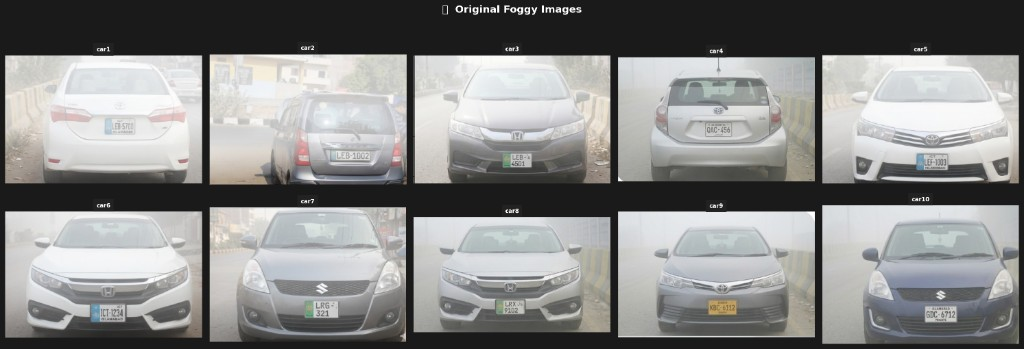
\includegraphics[width=\textwidth]{figures/pre/pre_input_foggy.png}
\caption{Original foggy uploads (ten-vehicle grid) prior to restoration.}
\label{fig:preinputfog}
\end{figure*}

\begin{figure*}[!tb]
\centering
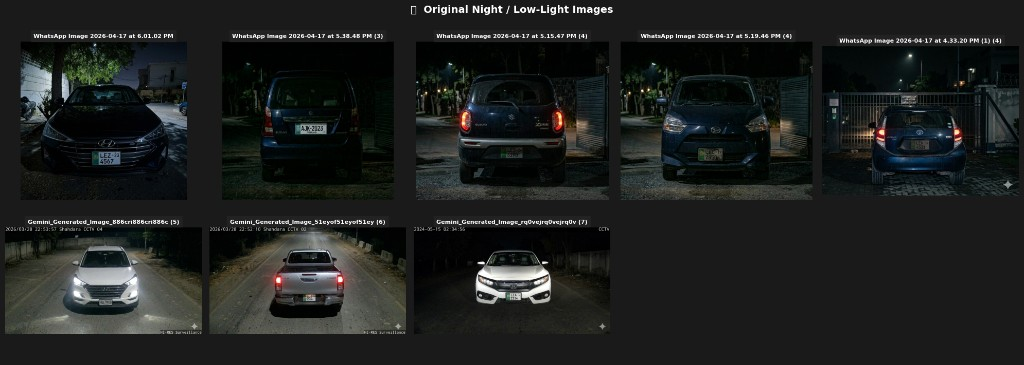
\includegraphics[width=\textwidth]{figures/pre/pre_input_night.png}
\caption{Original night / low-light set prior to restoration.}
\label{fig:preinputnight}
\end{figure*}

\begin{figure*}[!tb]
\centering
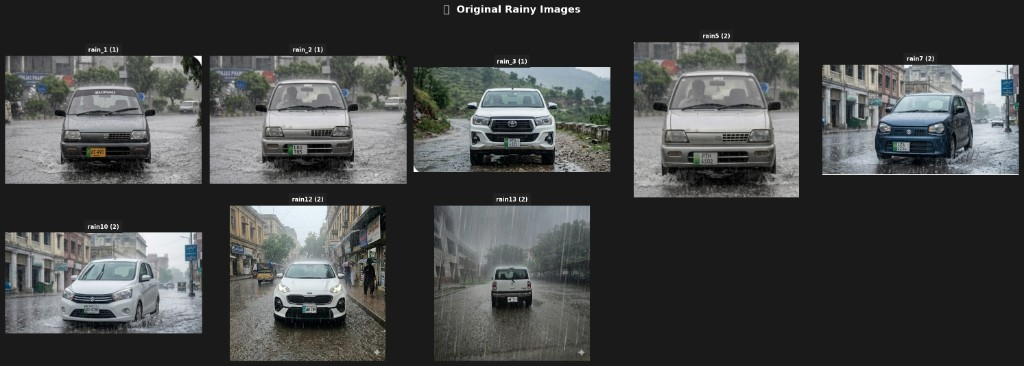
\includegraphics[width=\textwidth]{figures/pre/pre_input_rainy.png}
\caption{Original rainy scenes prior to restoration.}
\label{fig:preinputrain}
\end{figure*}

\begin{figure*}[!tb]
\centering
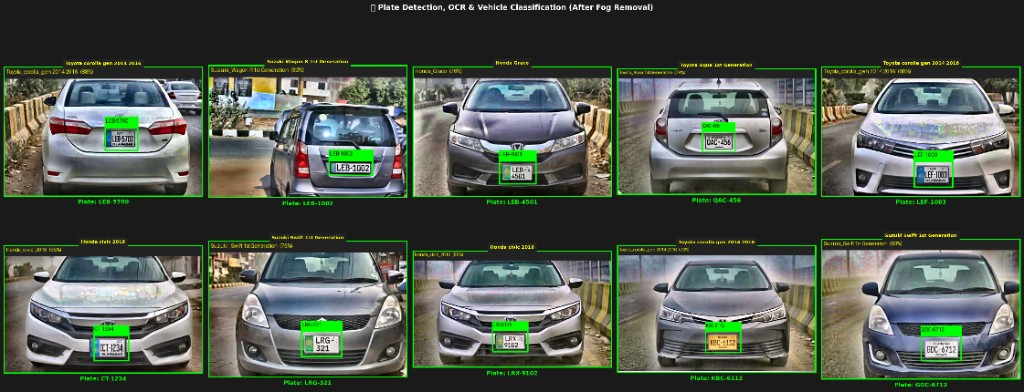
\includegraphics[width=\textwidth]{figures/pre/pre_pipeline_defog.png}
\caption{After fog removal + LPD + OCR + VMMR (overlays on restored imagery).}
\label{fig:prepipefog}
\end{figure*}

\begin{figure*}[!tb]
\centering
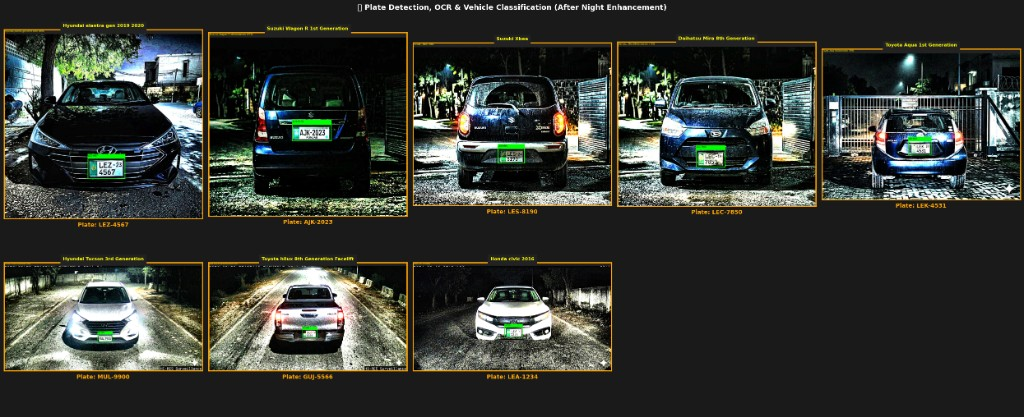
\includegraphics[width=\textwidth]{figures/pre/pre_pipeline_night.png}
\caption{After night enhancement + LPD + OCR + VMMR.}
\label{fig:prepipenight}
\end{figure*}

\begin{figure*}[!tb]
\centering
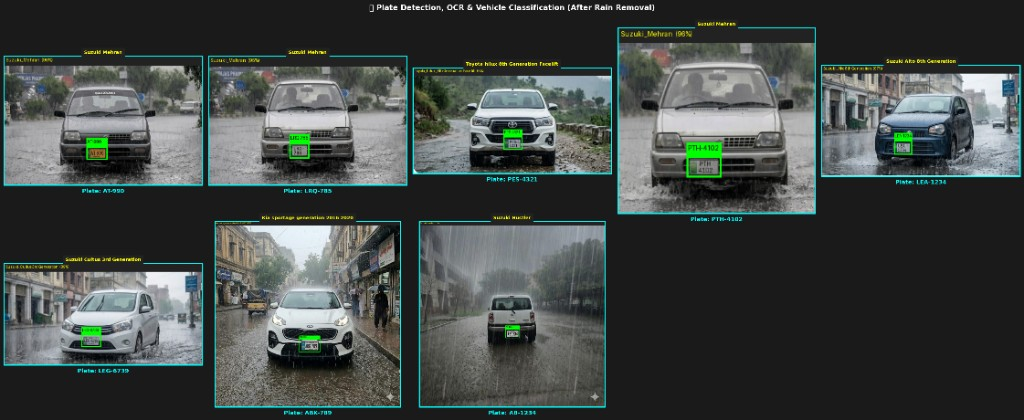
\includegraphics[width=\textwidth]{figures/pre/pre_pipeline_rain.png}
\caption{After rain removal + LPD + OCR + VMMR.}
\label{fig:prepiperain}
\end{figure*}

\paragraph{Plate localization montages.}\label{subsec:lpdmontage}
These small tiles are early prediction exports so readers see detector behavior before the full LPD charts below.

\begin{figure*}[!tb]
\centering

\begin{subfigure}[b]{0.23\textwidth}\centering
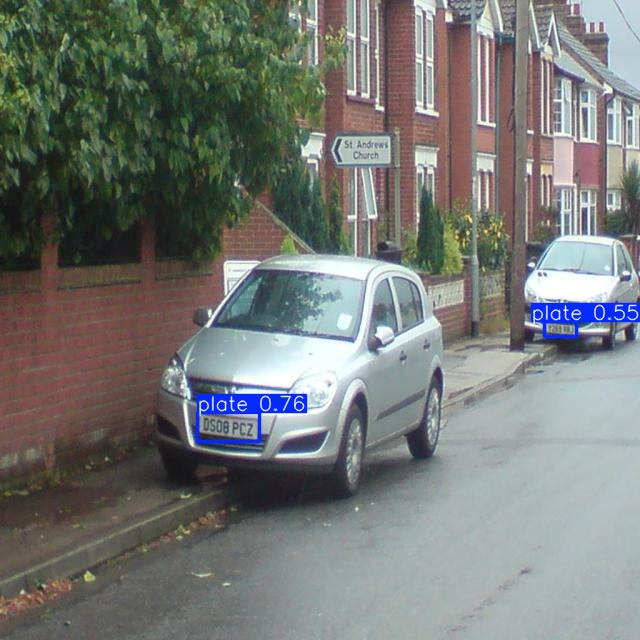
\includegraphics[width=\linewidth]{0002a5b67e5f0909_jpg.rf.300ba325f1e5e11ec6fdb10e70d11f4b.jpg}
\caption{Sample 1}
\end{subfigure}\hfil
\begin{subfigure}[b]{0.23\textwidth}\centering
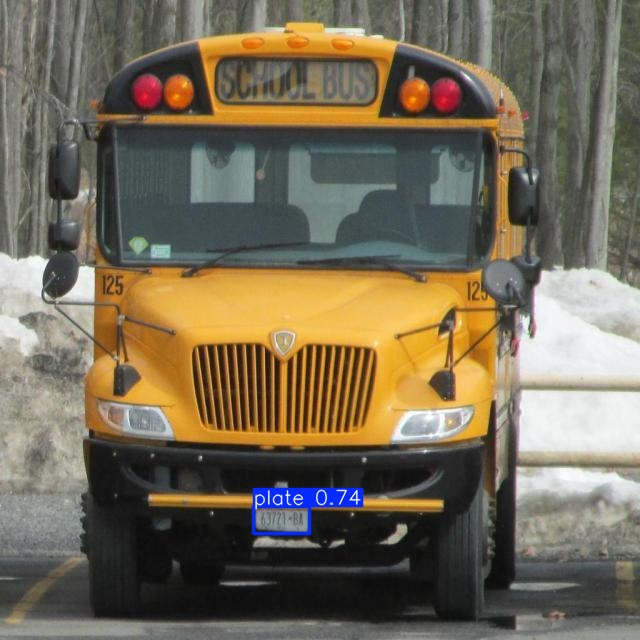
\includegraphics[width=\linewidth]{000812dcf304a8e7_jpg.rf.f0b445cb199333b34743798d98cdb57b.jpg}
\caption{Sample 2}
\end{subfigure}\hfil
\begin{subfigure}[b]{0.23\textwidth}\centering
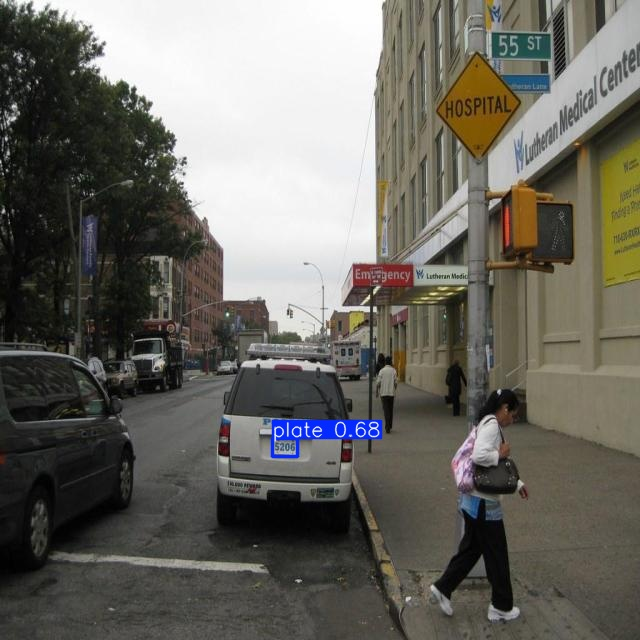
\includegraphics[width=\linewidth]{0010f4c10f7ab07e_jpg.rf.6aa0a7fccae068586c77cd9b3a165cbb.jpg}
\caption{Sample 3}
\end{subfigure}\hfil
\begin{subfigure}[b]{0.23\textwidth}\centering
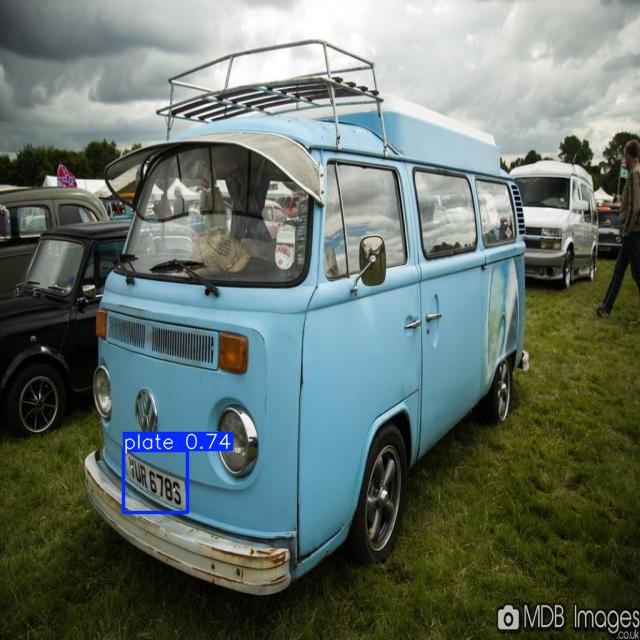
\includegraphics[width=\linewidth]{002519f868563098_jpg.rf.747ddee18711caaf4eec8c2788f18a53.jpg}
\caption{Sample 4}
\end{subfigure}\hfil
\caption{Early YOLOv8n plate-detection exports on Roboflow validation tiles: green boxes show predicted plate regions at confidence 0.25 on (a) daylight sedan, (b) angled hatchback, (c) partial occlusion, and (d) parking-lot view.}
\label{fig:y1}
\end{figure*}

\begin{figure*}[!tb]
\centering

\begin{subfigure}[b]{0.23\textwidth}\centering
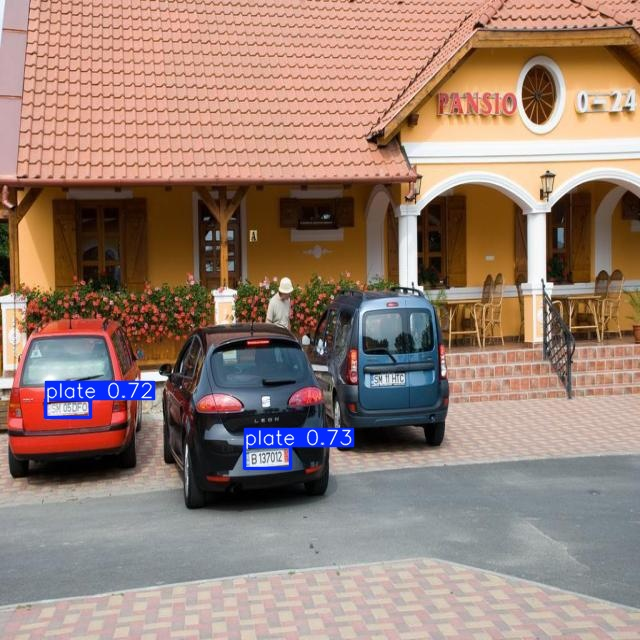
\includegraphics[width=\linewidth]{0026c246d5c33bea_jpg.rf.5e4c872c6b719cf9461250e4a548bbcf.jpg}
\caption{Sample 5}
\end{subfigure}\hfil
\begin{subfigure}[b]{0.23\textwidth}\centering
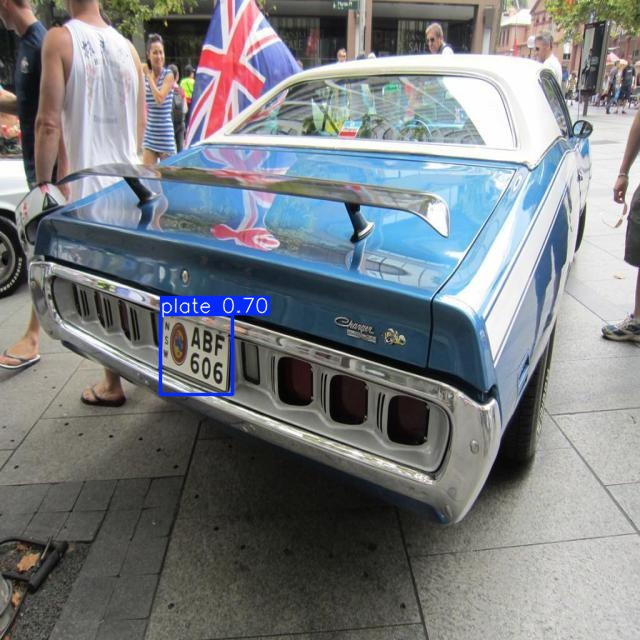
\includegraphics[width=\linewidth]{002901d9d194c4fb_jpg.rf.abb32cb00d3bfe6ccdd63b347f757453.jpg}
\caption{Sample 6}
\end{subfigure}\hfil
\begin{subfigure}[b]{0.23\textwidth}\centering
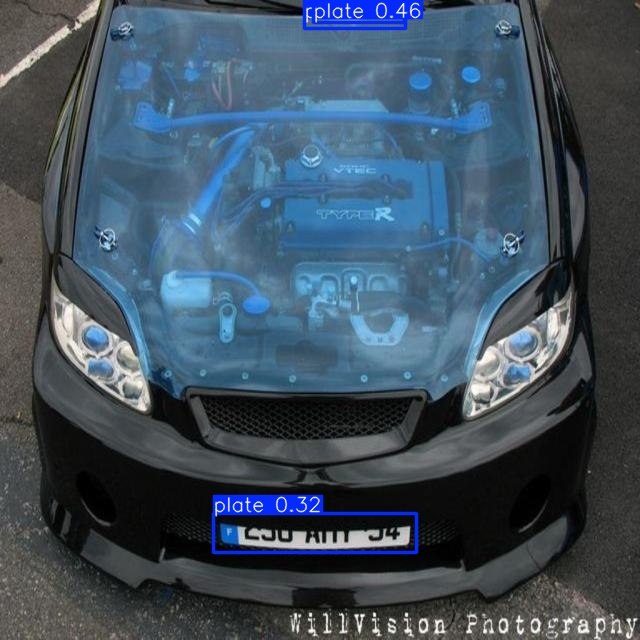
\includegraphics[width=\linewidth]{002d099996f3f443_jpg.rf.9dbeeab320aba1154957f121fc9be439.jpg}
\caption{Sample 7}
\end{subfigure}\hfil
\begin{subfigure}[b]{0.23\textwidth}\centering
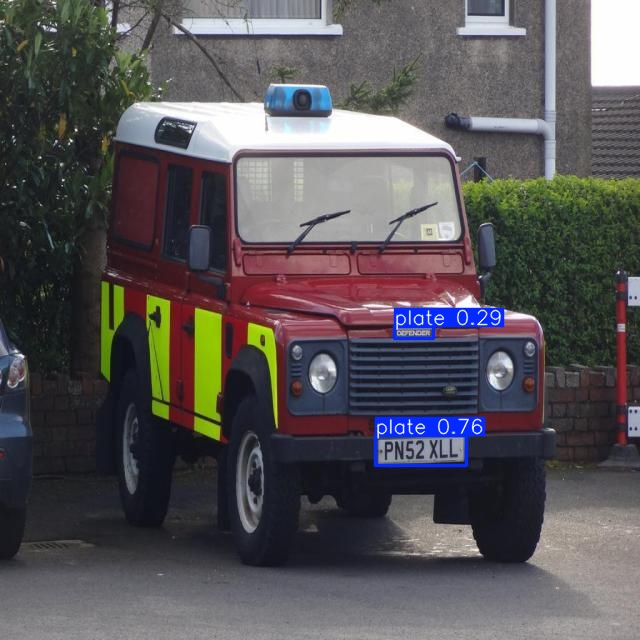
\includegraphics[width=\linewidth]{0039ac4bfb8bd69d_jpg.rf.e84acbf2cb5a4572116b702c1ef86857.jpg}
\caption{Sample 8}
\end{subfigure}\hfil
\caption{Additional plate-detection exports under varied viewpoints: (a)--(d) show single-plate hits; note consistent box aspect ratios across lighting changes.}
\label{fig:y4}
\end{figure*}

\begin{figure*}[!tb]
\centering

\begin{subfigure}[b]{0.23\textwidth}\centering
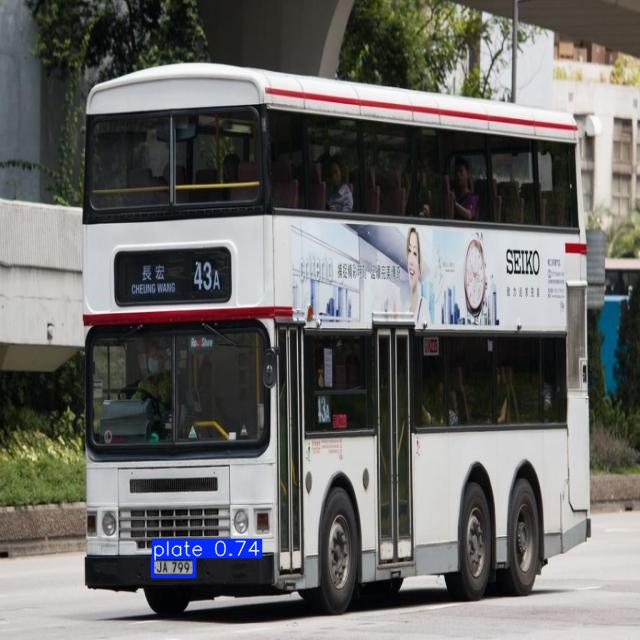
\includegraphics[width=\linewidth]{005e1faed531ae7e_jpg.rf.249fb183d641dec499d8e6d4e53f0378.jpg}
\caption{Export 9}
\end{subfigure}\hfil
\begin{subfigure}[b]{0.23\textwidth}\centering
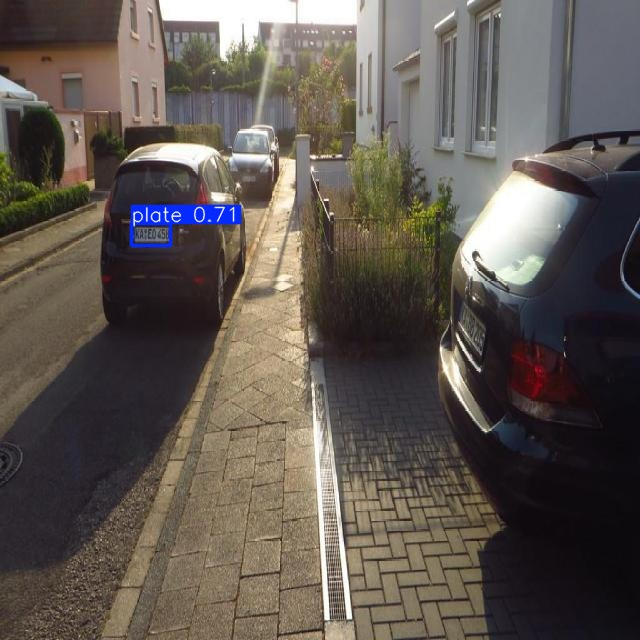
\includegraphics[width=\linewidth]{0063e41b53567829_jpg.rf.686da0392b4f487124f93b36ec386773.jpg}
\caption{Export 10}
\end{subfigure}\hfil
\begin{subfigure}[b]{0.23\textwidth}\centering
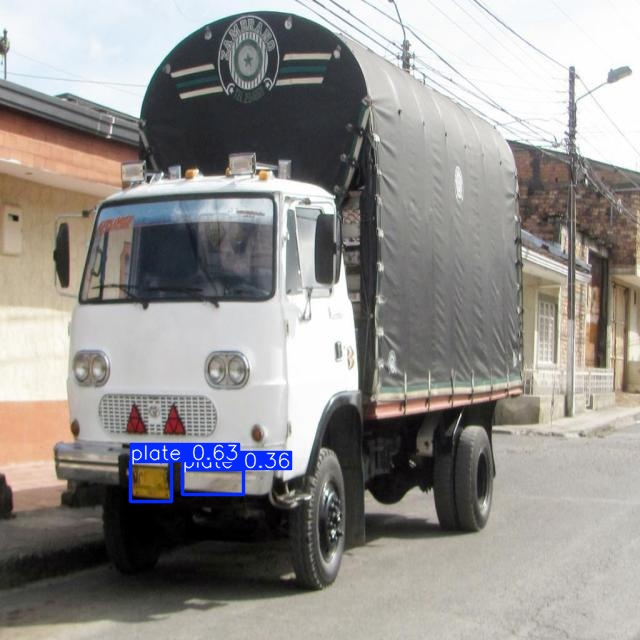
\includegraphics[width=\linewidth]{006a2f13b5b16c64_jpg.rf.a15e157b63c3debfb326174f156f882b.jpg}
\caption{Export 11}
\end{subfigure}\hfil
\begin{subfigure}[b]{0.23\textwidth}\centering
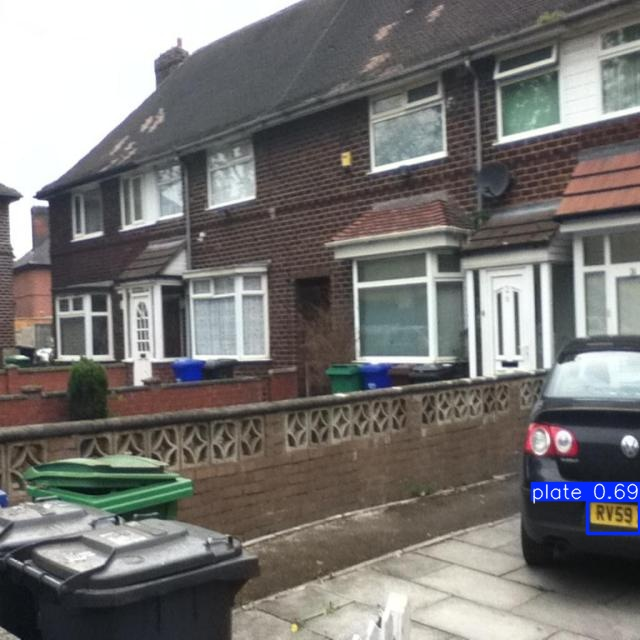
\includegraphics[width=\linewidth]{00777823afff31f7_jpg.rf.4ab8065d7faf8141a75a0c10cd94b211.jpg}
\caption{Export 12}
\end{subfigure}\hfil
\caption{Supplementary LPD qualitative tiles: (a)--(d) include low-contrast and multi-vehicle scenes used for informal regression checks before epoch~50 validation.}
\label{fig:yextra}
\end{figure*}

\paragraph{License Plate Detection (LPD) visual and diagnostic results.}\label{subsec:lpdfigs}
Figures~\ref{fig:lpdqual1}--\ref{fig:lpdqual2} mix daylight sedans, rainy night frames, parking-lot dual plates, and a highway zoom-out. Figure~\ref{fig:lpdheatmap} is a Colab-exported heatmap at $640{\times}640$ with confidence 0.25; use it beside---not instead of---the official epoch~50 validation in Table~\ref{tab:lpdmetrics}. Figures~\ref{fig:lpdvalbatch}--\ref{fig:lpdconf} add batch mosaics, label histograms, 50-epoch curves, PR diagnostics, and confusion summaries straight from Ultralytics.

\begin{figure*}[!tb]
\centering
\begin{subfigure}[b]{0.32\textwidth}\centering
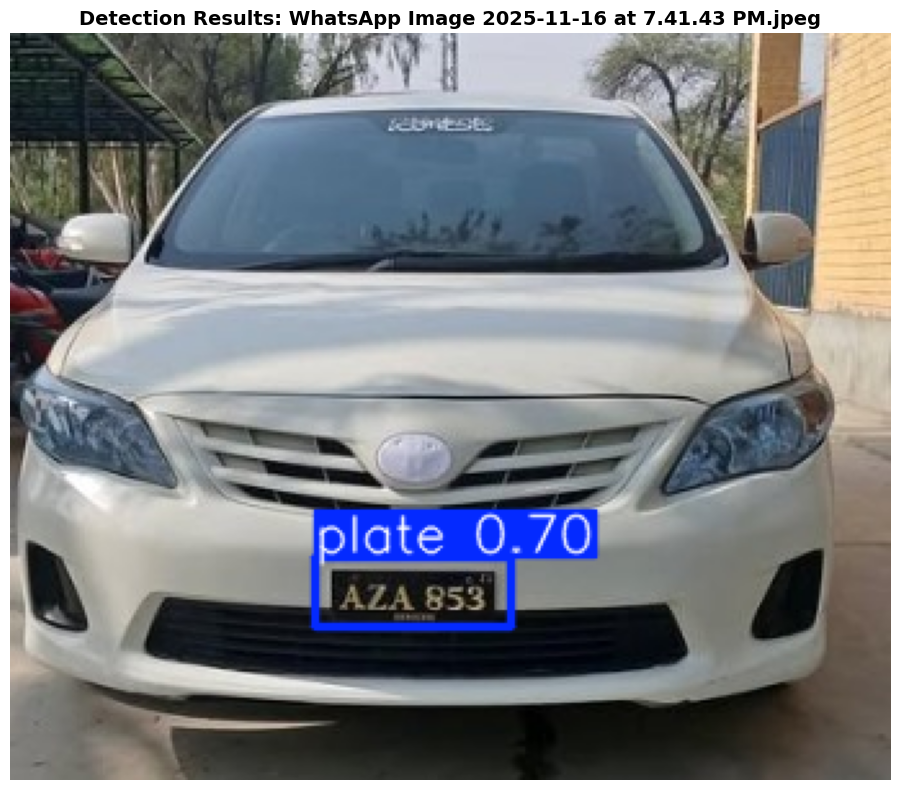
\includegraphics[width=\linewidth]{figures/lpd/lpd_pred_clear_corolla.png}
\caption{Clear daylight (frontal sedan).}
\end{subfigure}\hfil
\begin{subfigure}[b]{0.32\textwidth}\centering
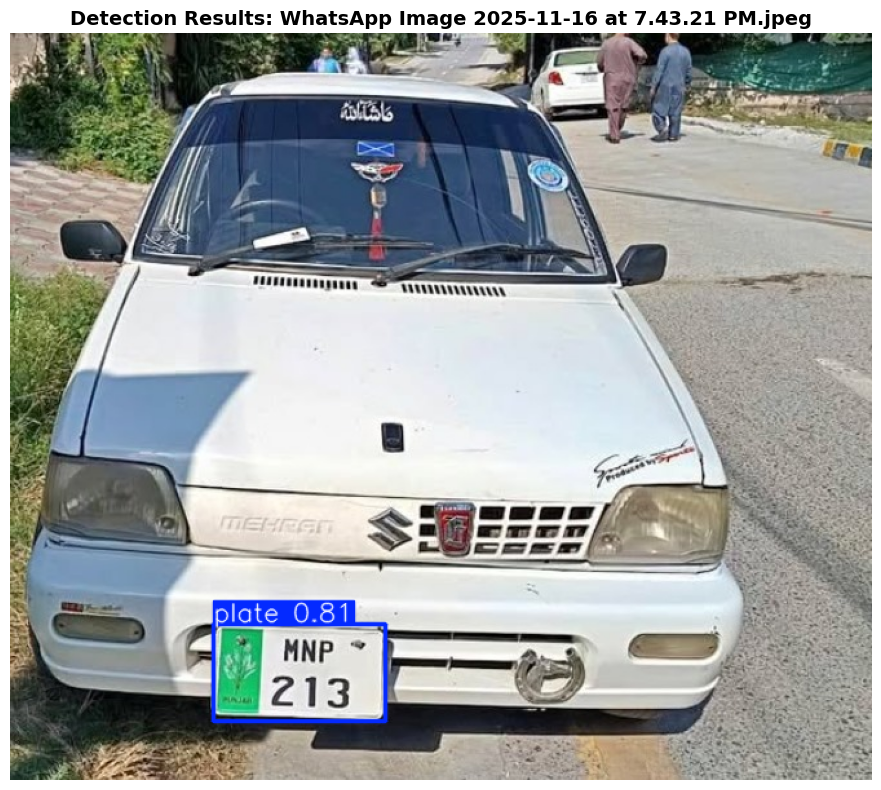
\includegraphics[width=\linewidth]{figures/lpd/lpd_pred_clear_mehran.png}
\caption{Clear daylight (regional plate styling).}
\end{subfigure}\hfil
\begin{subfigure}[b]{0.32\textwidth}\centering
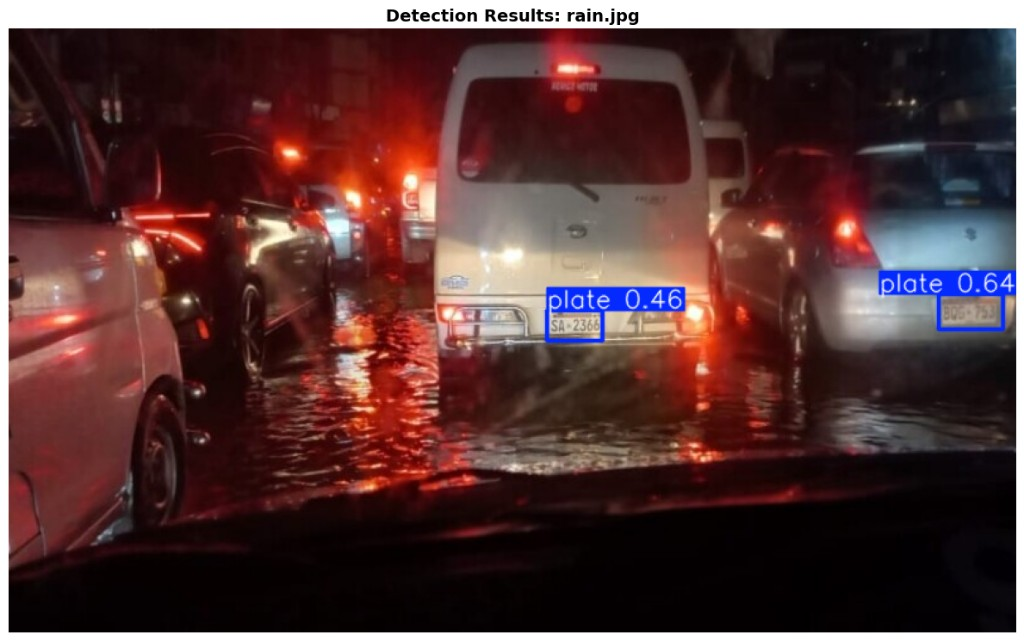
\includegraphics[width=\linewidth]{figures/lpd/lpd_pred_rain_night.png}
\caption{Night rain / glare (two detections).}
\end{subfigure}
\caption{Qualitative LPD outputs (bounding boxes and confidences overlaid by Ultralytics).}
\label{fig:lpdqual1}
\end{figure*}

\begin{figure*}[!tb]
\centering
\begin{subfigure}[b]{0.48\textwidth}\centering
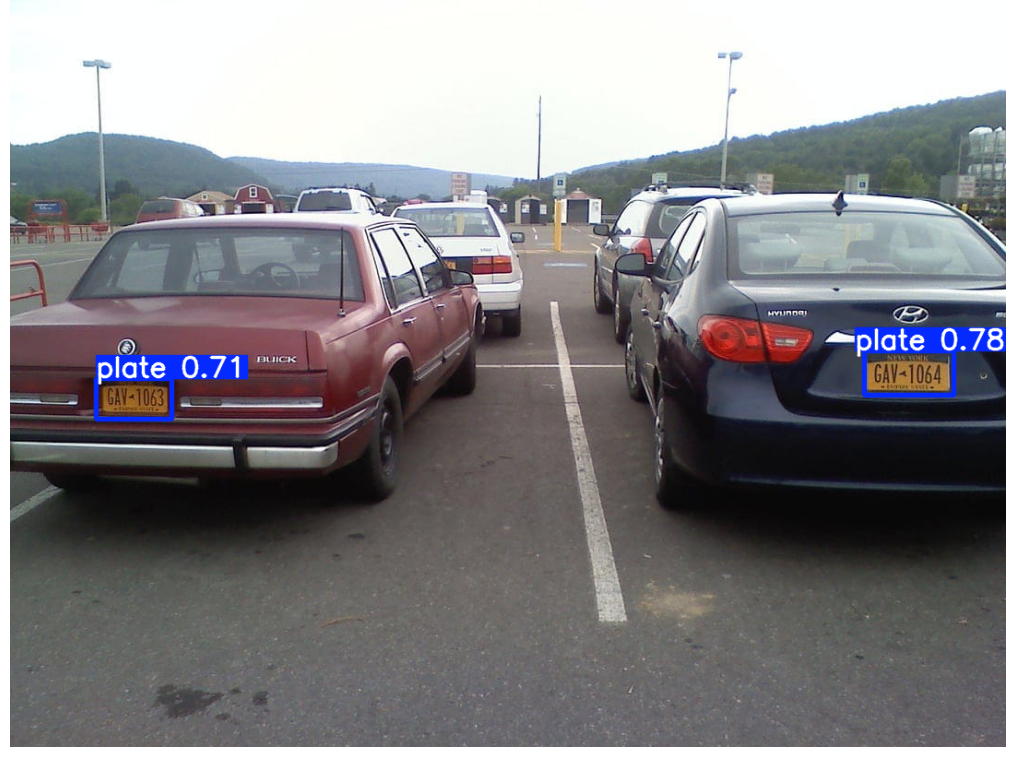
\includegraphics[width=\linewidth]{figures/lpd/lpd_pred_parking_dual.png}
\caption{Parking-lot dual plates.}
\end{subfigure}\hfil
\begin{subfigure}[b]{0.48\textwidth}\centering
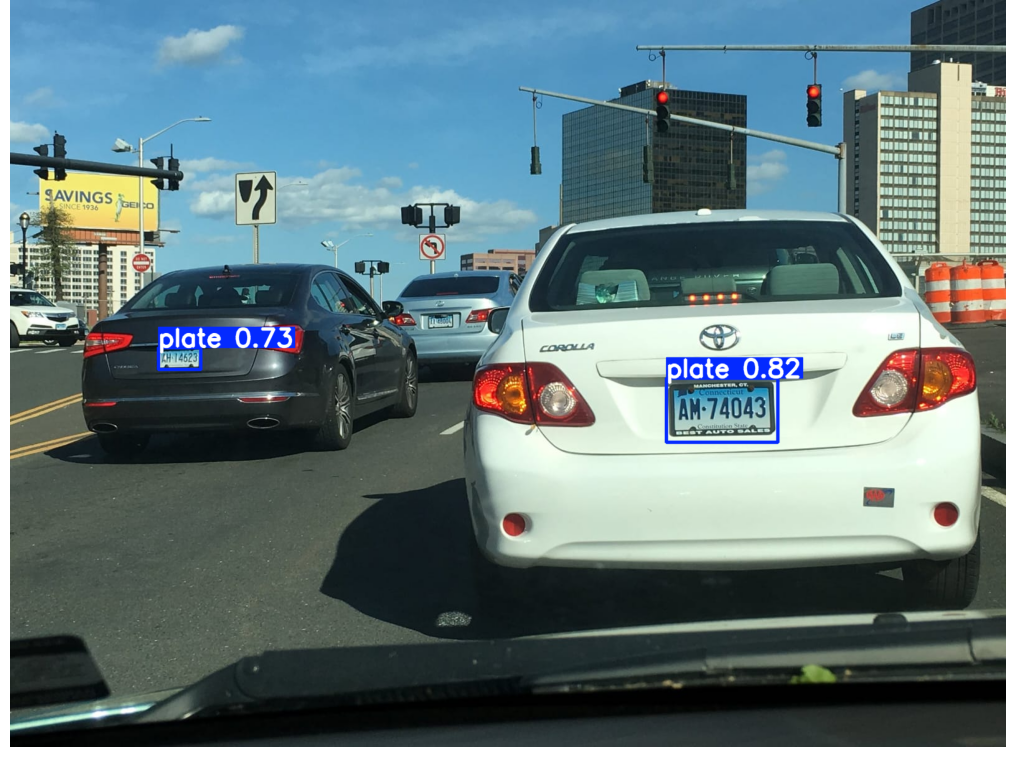
\includegraphics[width=\linewidth]{figures/lpd/lpd_pred_highway_dual.png}
\caption{Highway scene (multi-lane).}
\end{subfigure}
\caption{Additional qualitative LPD results under outdoor daylight.}
\label{fig:lpdqual2}
\end{figure*}

\begin{figure*}[!tb]
\centering
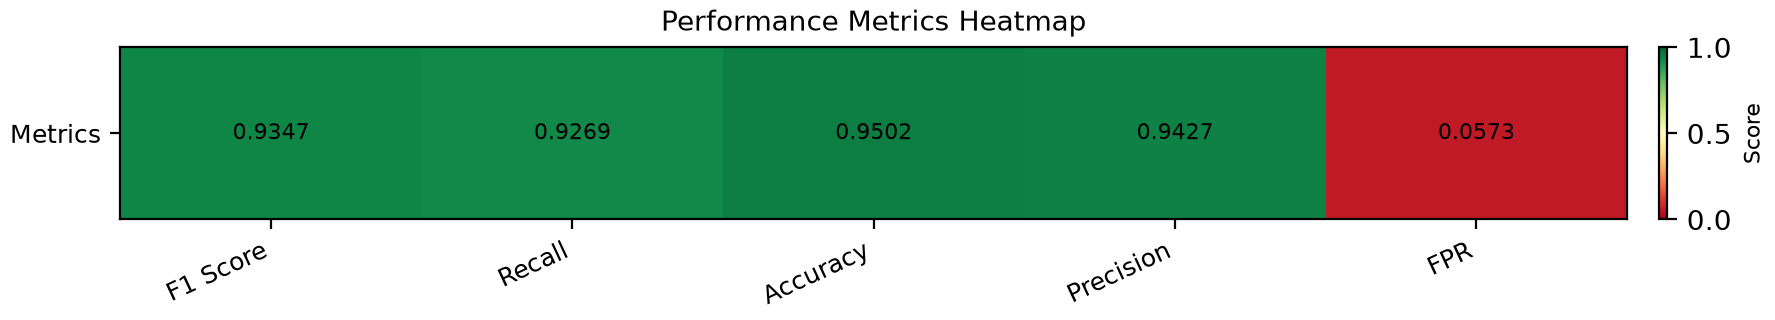
\includegraphics[width=0.82\textwidth]{figures/lpd/lpd_metrics_heatmap.png}
\caption{Scalar performance heatmap for LPD (validation export at $640\times640$, confidence 0.25).}
\label{fig:lpdheatmap}
\end{figure*}

\begin{figure*}[!tb]
\centering
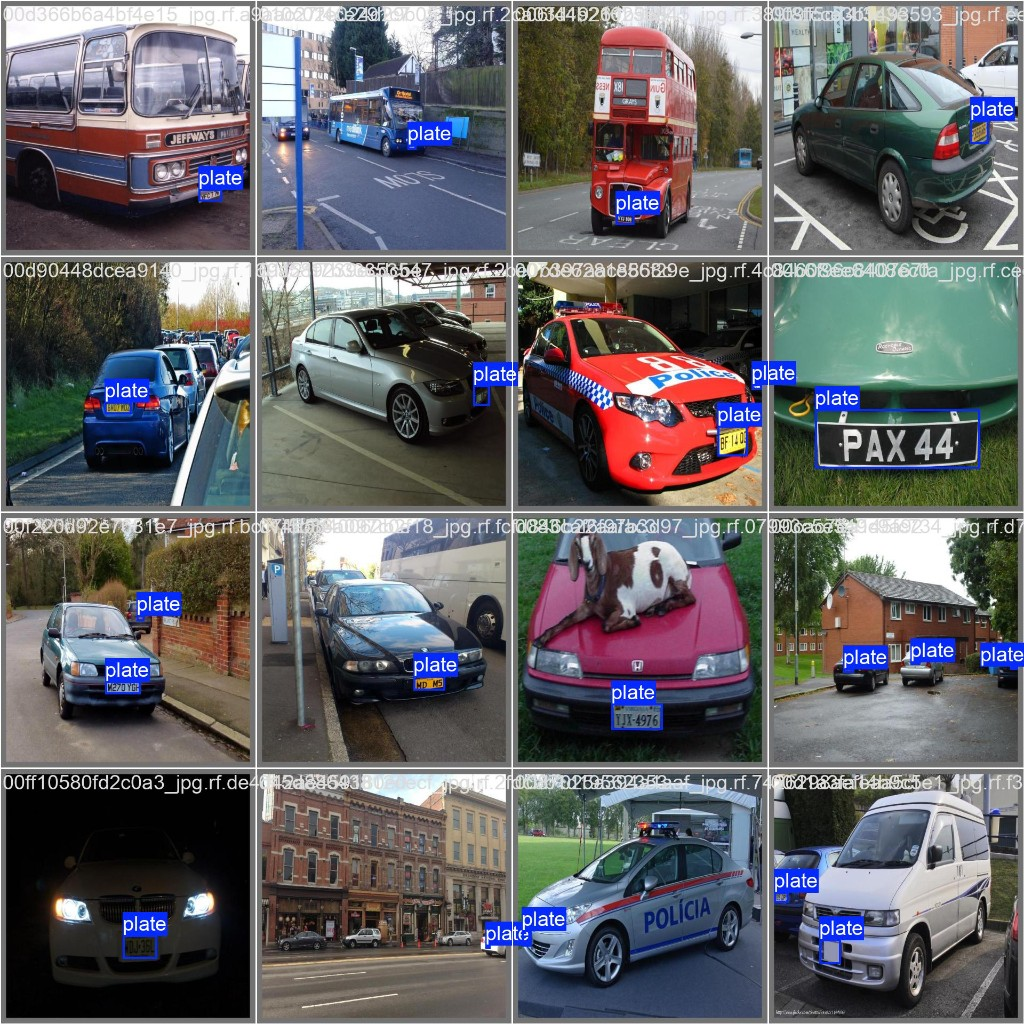
\includegraphics[width=0.95\linewidth]{figures/lpd/lpd_val_batch_labels.png}
\caption{Validation batch mosaic with ground-truth boxes (Roboflow-style tiles).}
\label{fig:lpdvalbatch}
\end{figure*}

\begin{figure*}[!tb]
\centering
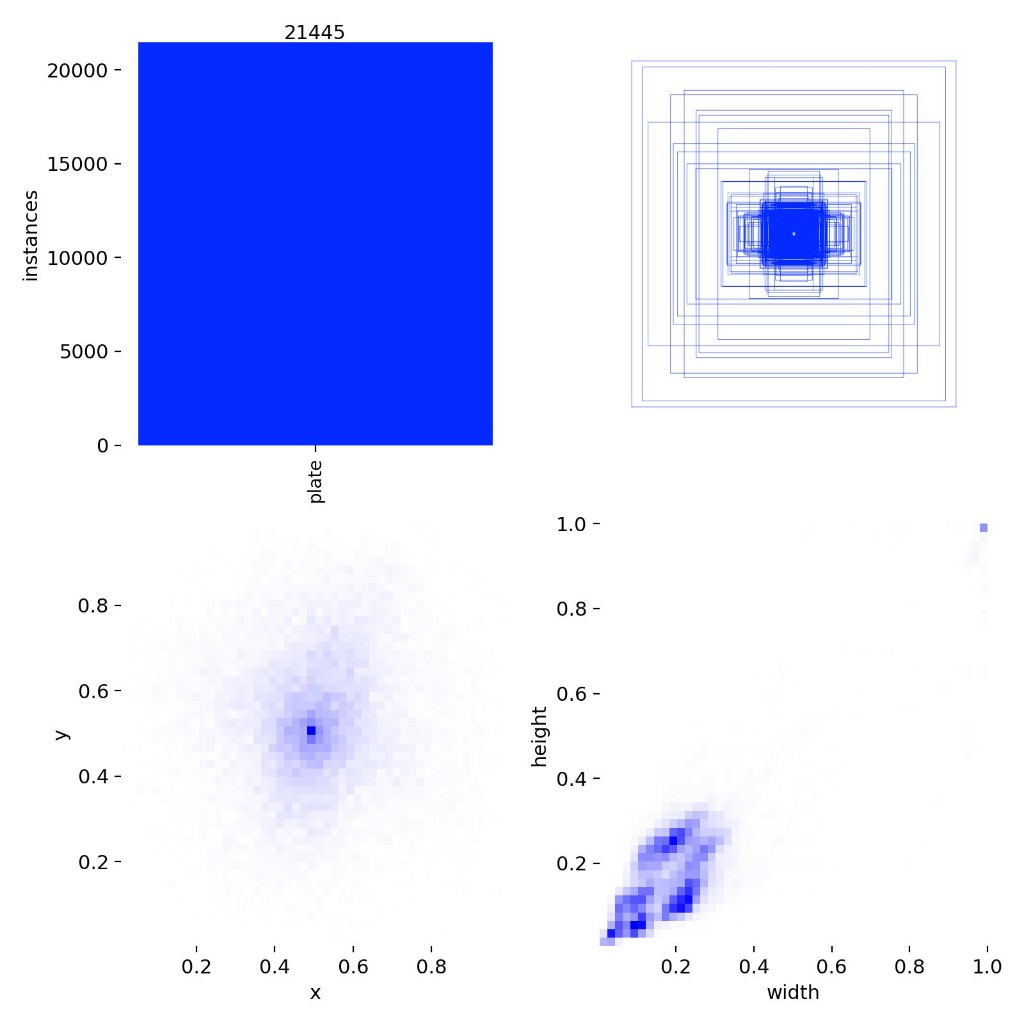
\includegraphics[width=0.95\linewidth]{figures/lpd/lpd_dataset_labels.png}
\caption{Dataset label analysis: class counts, box shapes, center and size heatmaps.}
\label{fig:lpddataset}
\end{figure*}

\begin{figure*}[!tb]
\centering
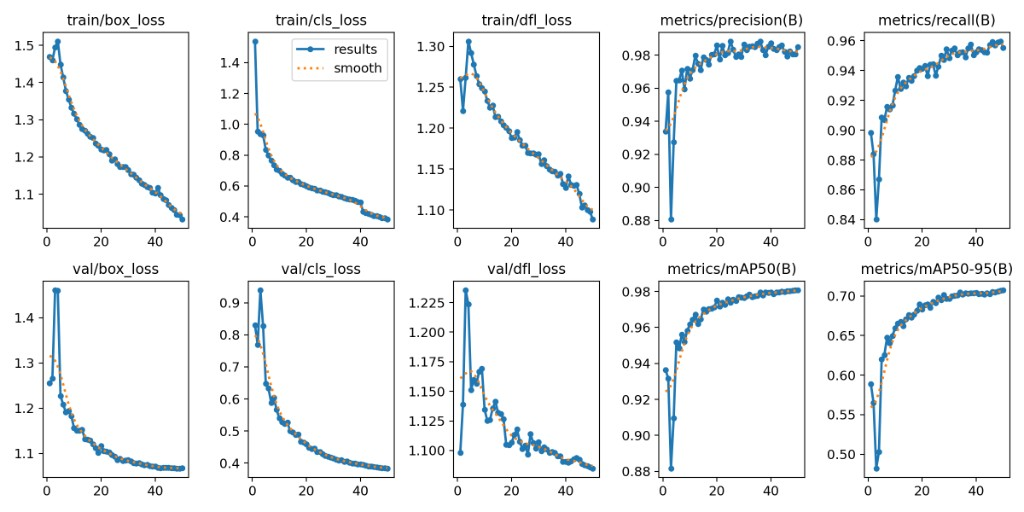
\includegraphics[width=\textwidth]{figures/lpd/lpd_training_results.png}
\caption{Training and validation losses plus Box precision, recall, mAP@0.5, and mAP@0.5:0.95 over 50 epochs.}
\label{fig:lpdtraincurves}
\end{figure*}

\begin{figure*}[!tb]
\centering
\begin{subfigure}[b]{0.48\textwidth}\centering
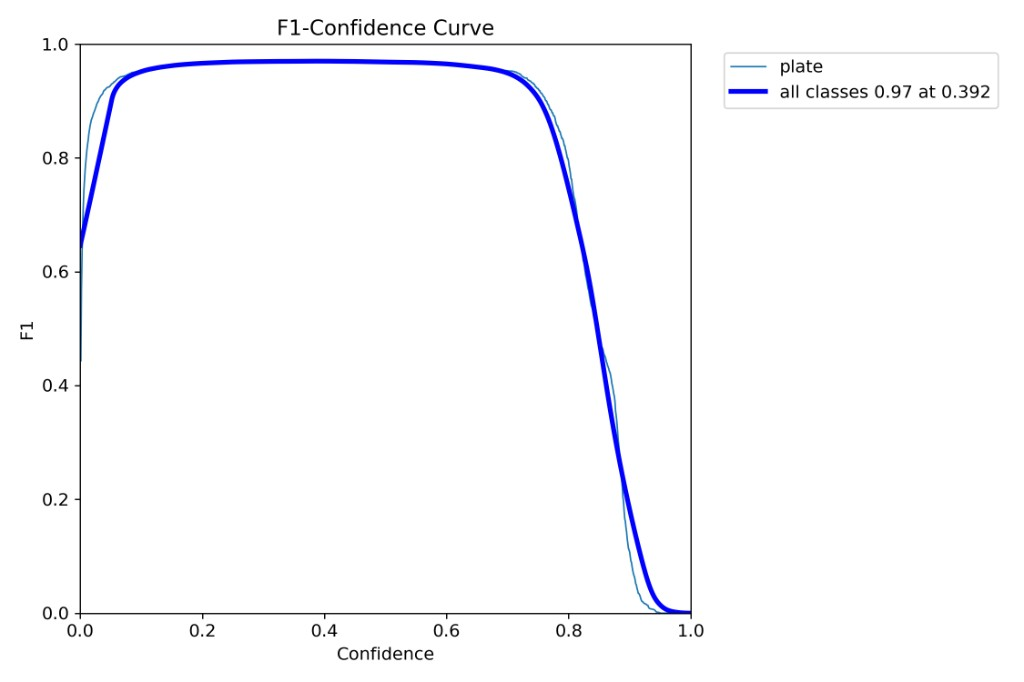
\includegraphics[width=\linewidth]{figures/lpd/lpd_curve_f1.png}
\caption{F1--confidence.}
\end{subfigure}\hfil
\begin{subfigure}[b]{0.48\textwidth}\centering
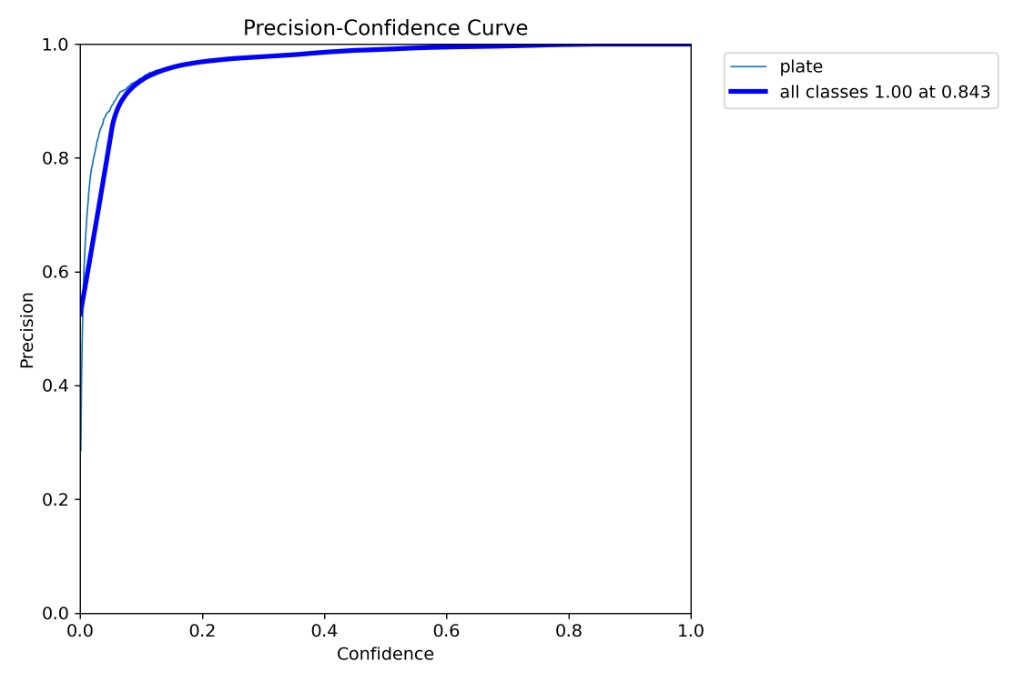
\includegraphics[width=\linewidth]{figures/lpd/lpd_curve_precision.png}
\caption{Precision--confidence.}
\end{subfigure}\\[1.5ex]
\begin{subfigure}[b]{0.48\textwidth}\centering
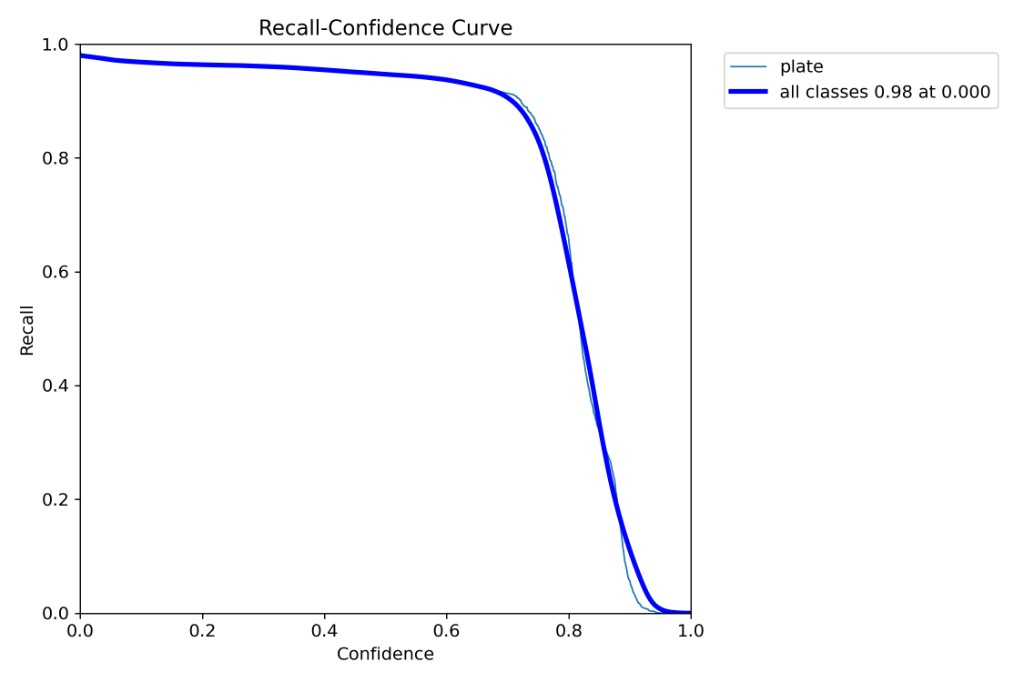
\includegraphics[width=\linewidth]{figures/lpd/lpd_curve_recall.png}
\caption{Recall--confidence.}
\end{subfigure}\hfil
\begin{subfigure}[b]{0.48\textwidth}\centering
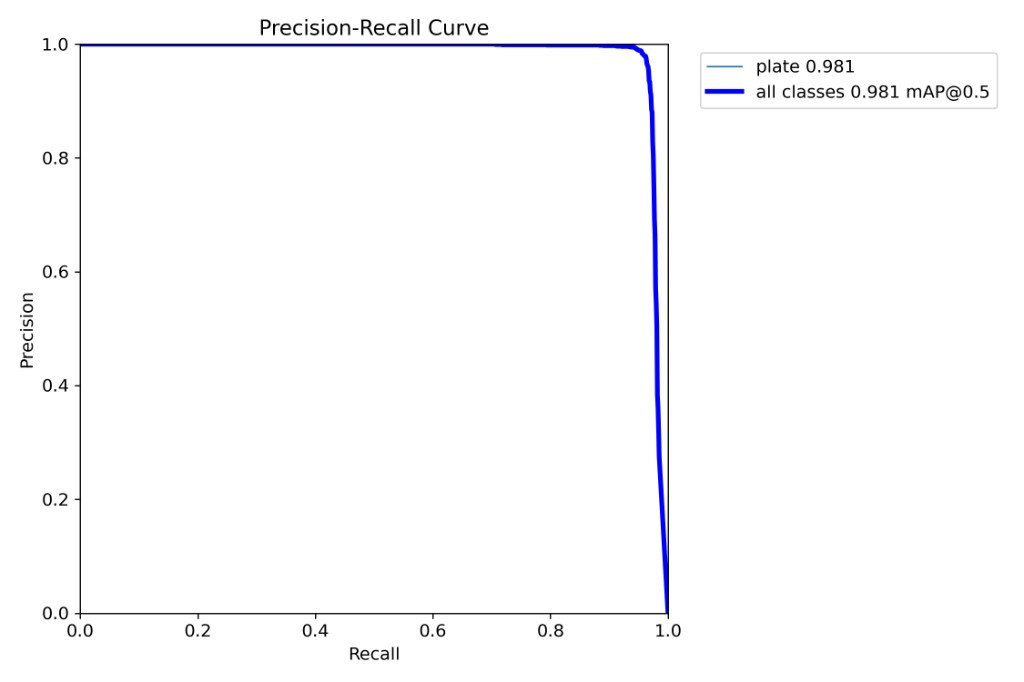
\includegraphics[width=\linewidth]{figures/lpd/lpd_curve_pr.png}
\caption{Precision--recall (AP / mAP@0.5).}
\end{subfigure}
\caption{Ultralytics diagnostic curves for the plate class.}
\label{fig:lpdcurves4}
\end{figure*}

\begin{figure*}[!tb]
\centering
\begin{subfigure}[b]{0.48\textwidth}\centering
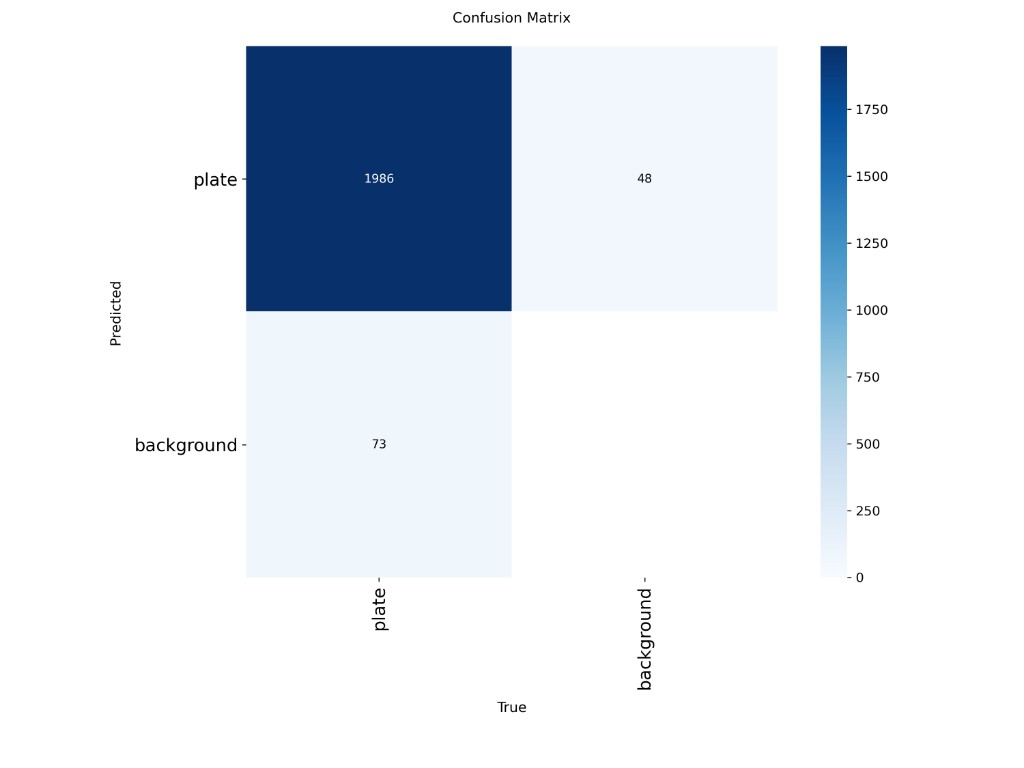
\includegraphics[width=\linewidth]{figures/lpd/lpd_confusion_matrix.png}
\caption{Counts confusion matrix.}
\end{subfigure}\hfil
\begin{subfigure}[b]{0.48\textwidth}\centering
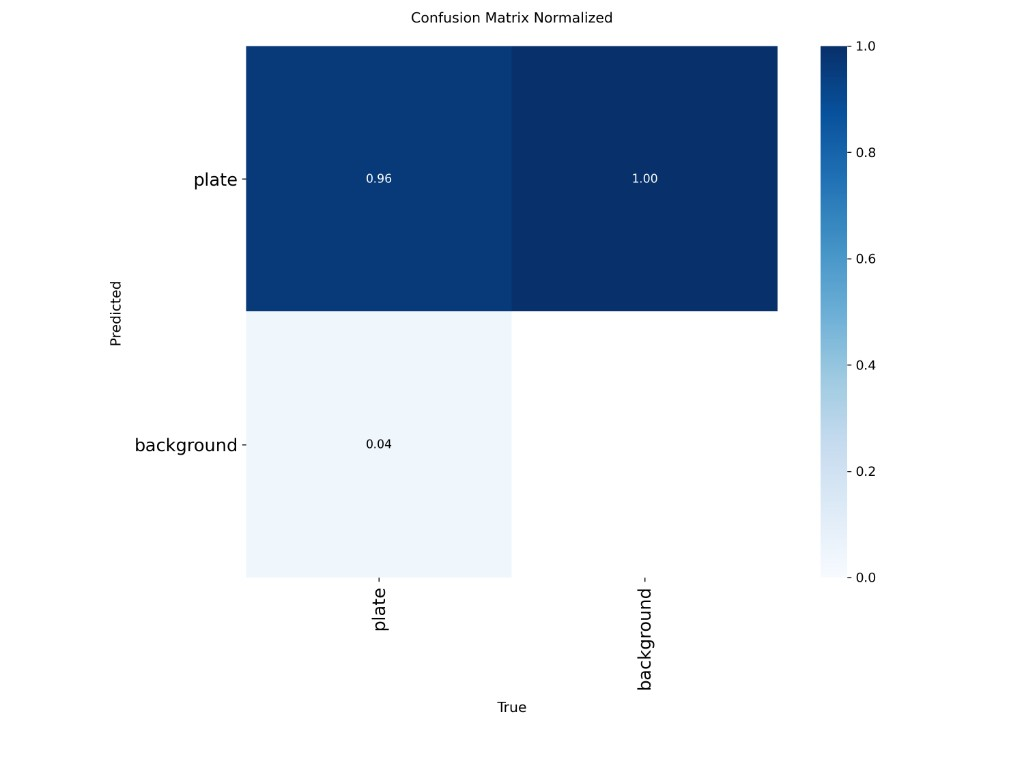
\includegraphics[width=\linewidth]{figures/lpd/lpd_confusion_normalized.png}
\caption{Normalized confusion matrix.}
\end{subfigure}
\caption{Confusion summaries for plate versus background.}
\label{fig:lpdconf}
\end{figure*}

\paragraph{License Plate Character and Digit Recognition (OCR) visual and diagnostic results.}\label{subsec:lpocrfigs}
Figures~\ref{fig:ocrmetrics}--\ref{fig:ocrtrain} summarize the YOLOv8n character detector: a validation-metrics heatmap, a batched validation label mosaic (Figure~\ref{fig:ocrvalbatch0}), qualitative glyph boxes on regional plate layouts, end-to-end readouts, Ultralytics diagnostic curves, confusion matrices, and the 100-epoch training trace. Headline scalars sit in Table~\ref{tab:lpcharmetrics}; remember Section~\ref{subsec:lpchar}: validation duplicated training images for this export.

\begin{figure*}[!tb]
\centering
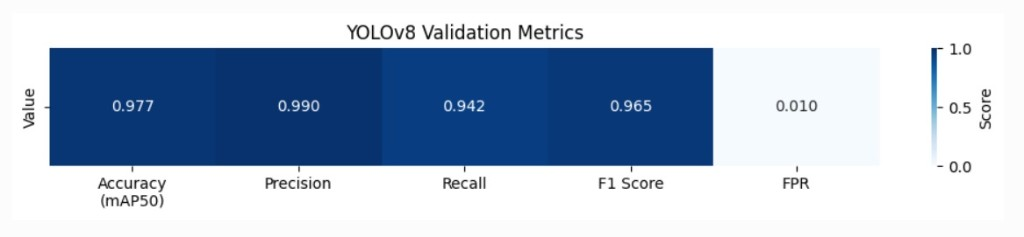
\includegraphics[width=0.82\textwidth]{figures/lpr_char/ocr_metrics_heatmap.png}
\caption{YOLOv8n character detection and recognition validation metrics heatmap at epoch~100: mAP@0.5 0.977, precision 0.990, recall 0.942, F1 0.965, and FPR 0.010 on the mirrored Roboflow v4 validation pool.}
\label{fig:ocrmetrics}
\end{figure*}

\begin{figure*}[!tb]
\centering
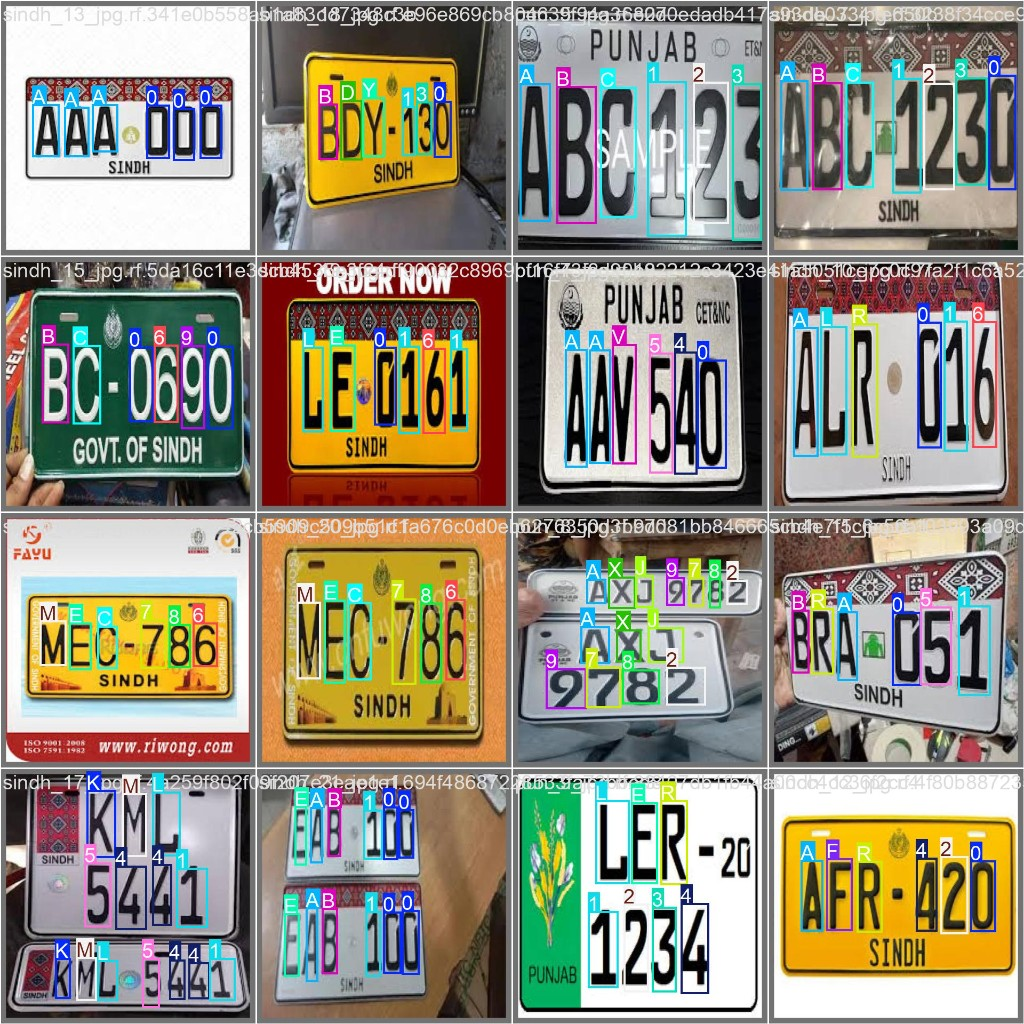
\includegraphics[width=0.72\textwidth]{figures/lpr_char/ocr_val_batch0_labels.png}
\caption{YOLOv8n character validation batch at epoch~100: ground-truth glyph boxes on Sindh and Punjab plate crops (Roboflow v4, 38 classes). Each tile shows class-coloured boxes with digit/letter labels above each character region.}
\label{fig:ocrvalbatch0}
\end{figure*}

\begin{figure*}[!tb]
\centering
\begin{subfigure}[b]{0.32\textwidth}\centering
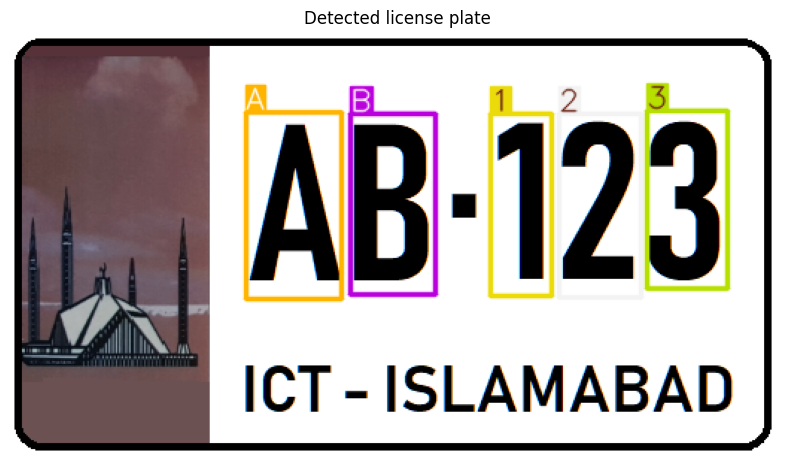
\includegraphics[width=\linewidth]{figures/lpr_char/ocr_qual_islamabad.png}
\caption{ICT (Islamabad) crop with per-glyph boxes.}
\end{subfigure}\hfil
\begin{subfigure}[b]{0.32\textwidth}\centering
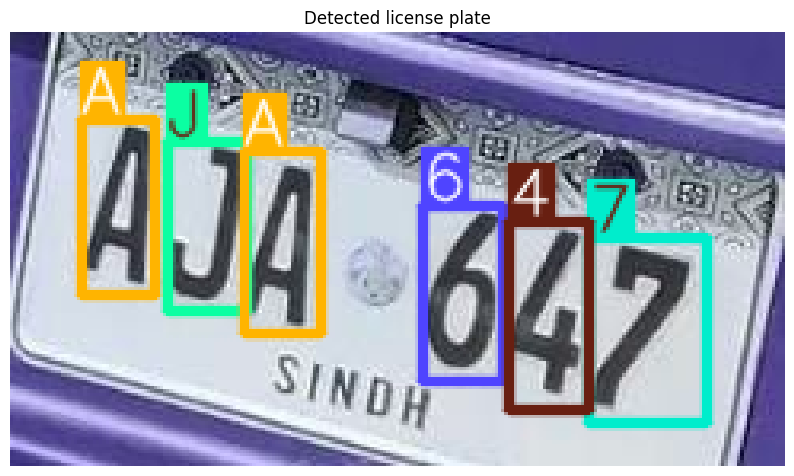
\includegraphics[width=\linewidth]{figures/lpr_char/ocr_qual_sindh_aja.png}
\caption{Sindh plate (three-letter, three-digit style readout).}
\end{subfigure}\hfil
\begin{subfigure}[b]{0.32\textwidth}\centering
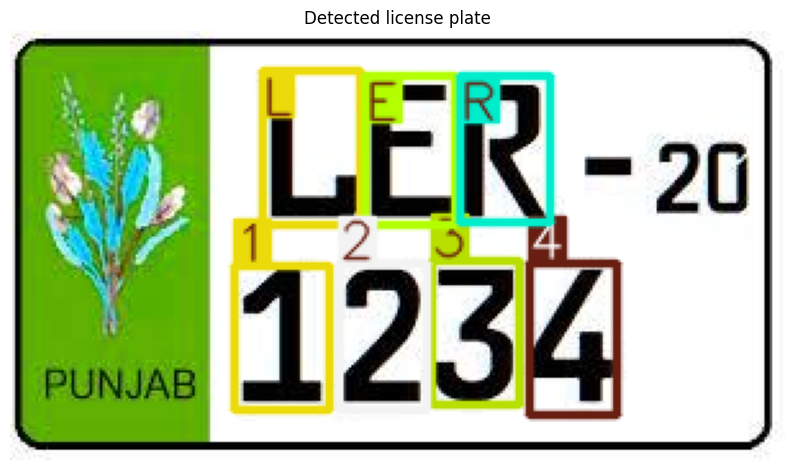
\includegraphics[width=\linewidth]{figures/lpr_char/ocr_qual_punjab_ler.png}
\caption{Punjab plate with stacked rows.}
\end{subfigure}
\caption{Qualitative character-level detections (YOLOv8n head, class-coloured boxes).}
\label{fig:ocrqual1}
\end{figure*}

\begin{figure*}[!tb]
\centering
\begin{subfigure}[b]{0.48\textwidth}\centering
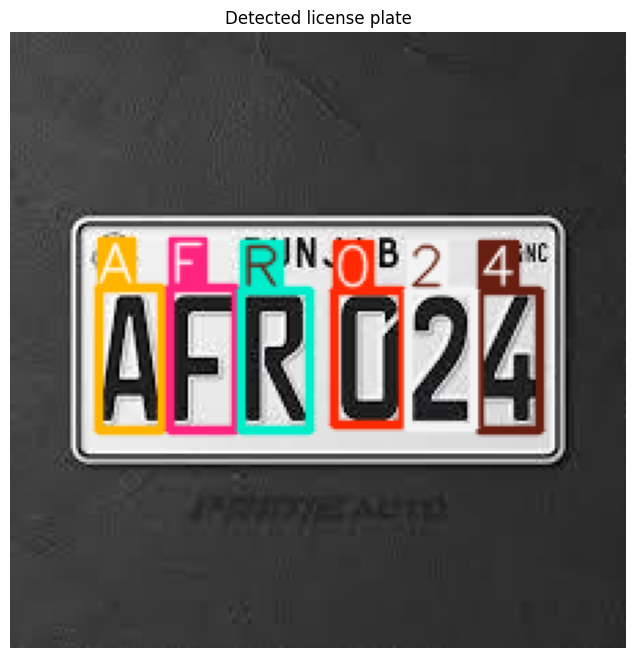
\includegraphics[width=\linewidth]{figures/lpr_char/ocr_qual_punjab_afr.png}
\caption{Punjab frontal crop (tight digit band).}
\end{subfigure}\hfil
\begin{subfigure}[b]{0.48\textwidth}\centering
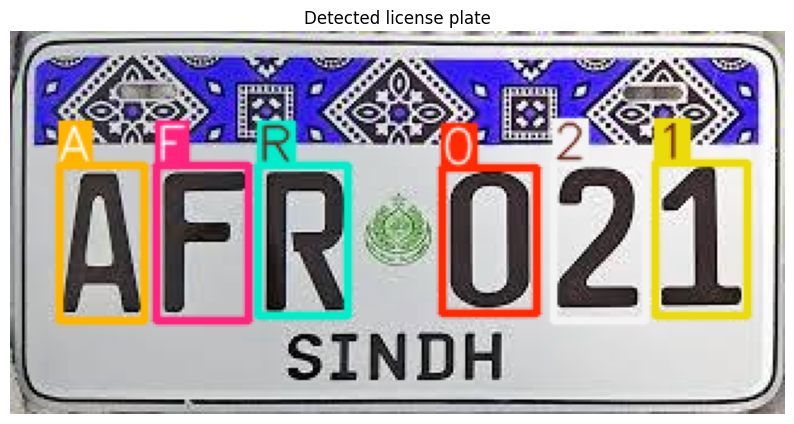
\includegraphics[width=\linewidth]{figures/lpr_char/ocr_qual_sindh_afr021.png}
\caption{Sindh variant with emblem spacing.}
\end{subfigure}
\caption{Additional qualitative OCR panels on contrasting layouts. In (a), several character proposals sit close on the same strokes, so Ultralytics-style text labels overlap in the export even when boxes are mostly correct. In (b), wider spacing and the emblem break up the band, so labels stay legible.}
\label{fig:ocrqual2}
\end{figure*}

\begin{figure*}[!tb]
\centering
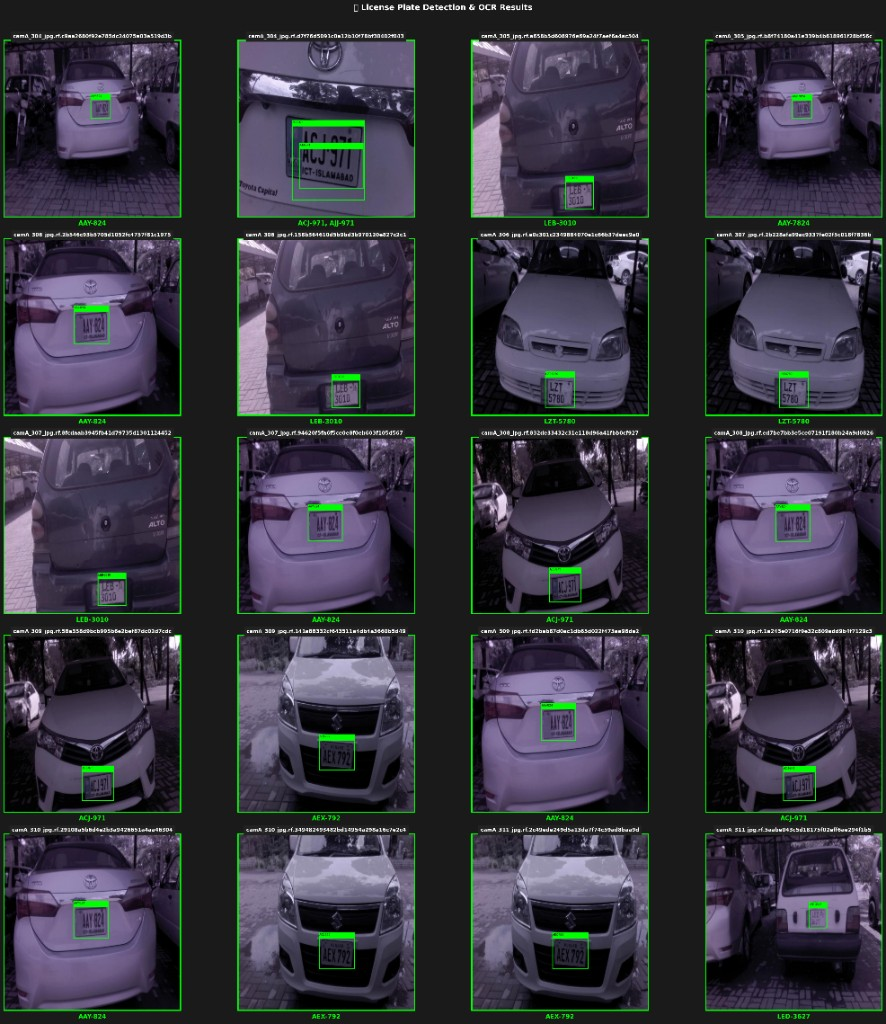
\includegraphics[width=\linewidth]{figures/lpr_char/ocr_e2e_plate_grid.png}
\caption{End-to-end detection and OCR readouts on sample vehicles (green plate boxes with predicted strings).}
\label{fig:ocre2e}
\end{figure*}

\begin{figure*}[!tb]
\centering
\begin{subfigure}[b]{0.48\textwidth}\centering
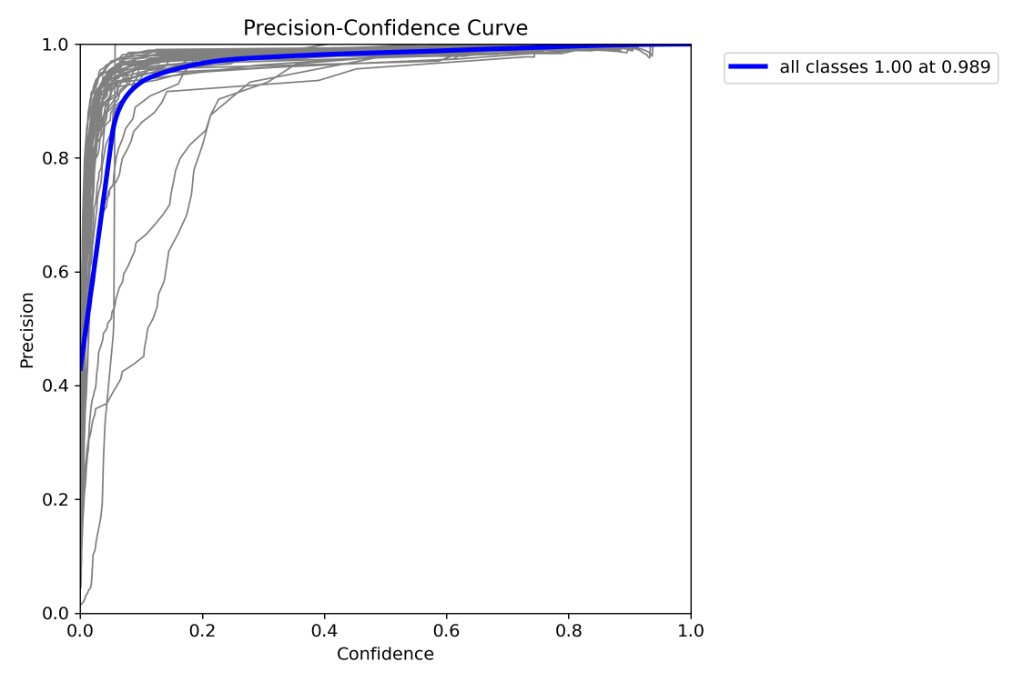
\includegraphics[width=\linewidth]{figures/lpr_char/ocr_boxP_curve.png}
\caption{Precision--confidence.}
\end{subfigure}\hfil
\begin{subfigure}[b]{0.48\textwidth}\centering
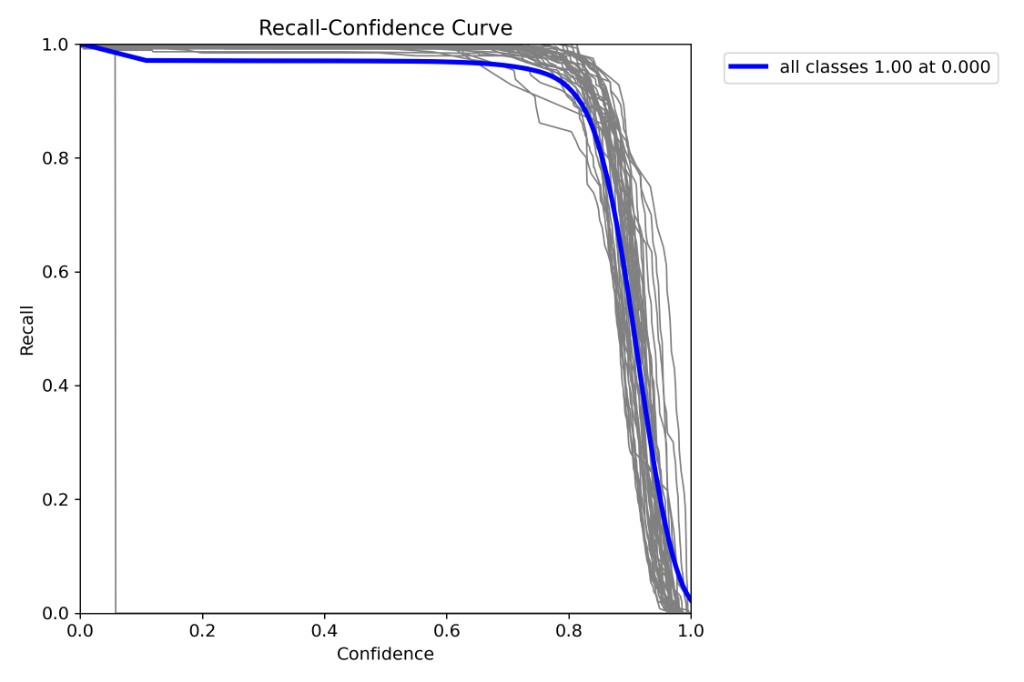
\includegraphics[width=\linewidth]{figures/lpr_char/ocr_boxR_curve.png}
\caption{Recall--confidence.}
\end{subfigure}\\[1.5ex]
\begin{subfigure}[b]{0.48\textwidth}\centering
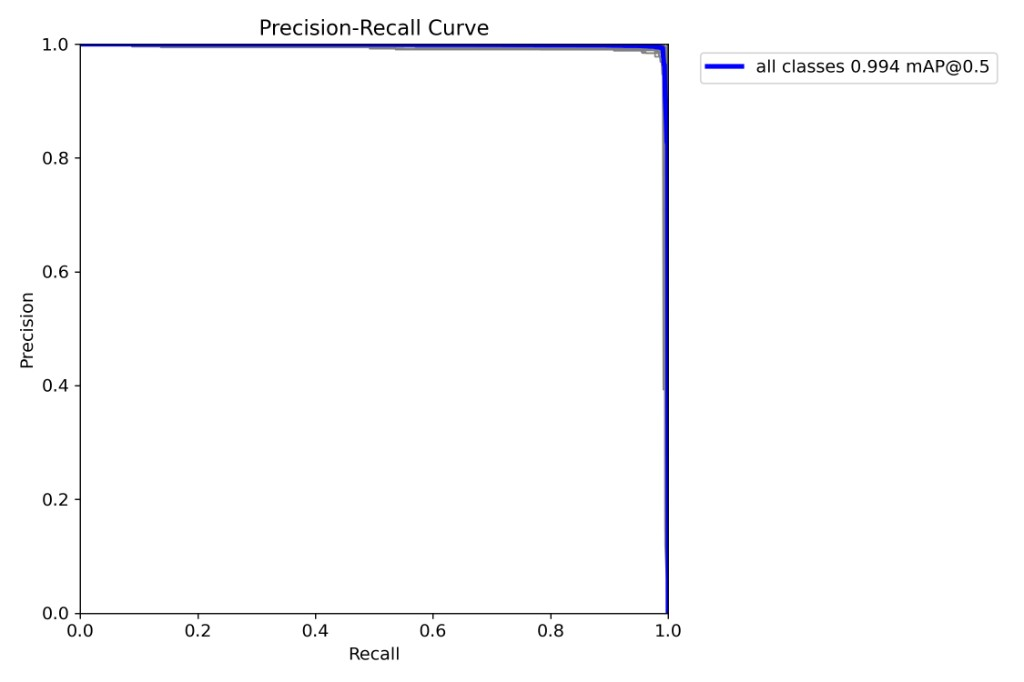
\includegraphics[width=\linewidth]{figures/lpr_char/ocr_boxPR_curve.png}
\caption{Precision--recall (mAP@0.5 legend per Ultralytics export).}
\end{subfigure}\hfil
\begin{subfigure}[b]{0.48\textwidth}\centering
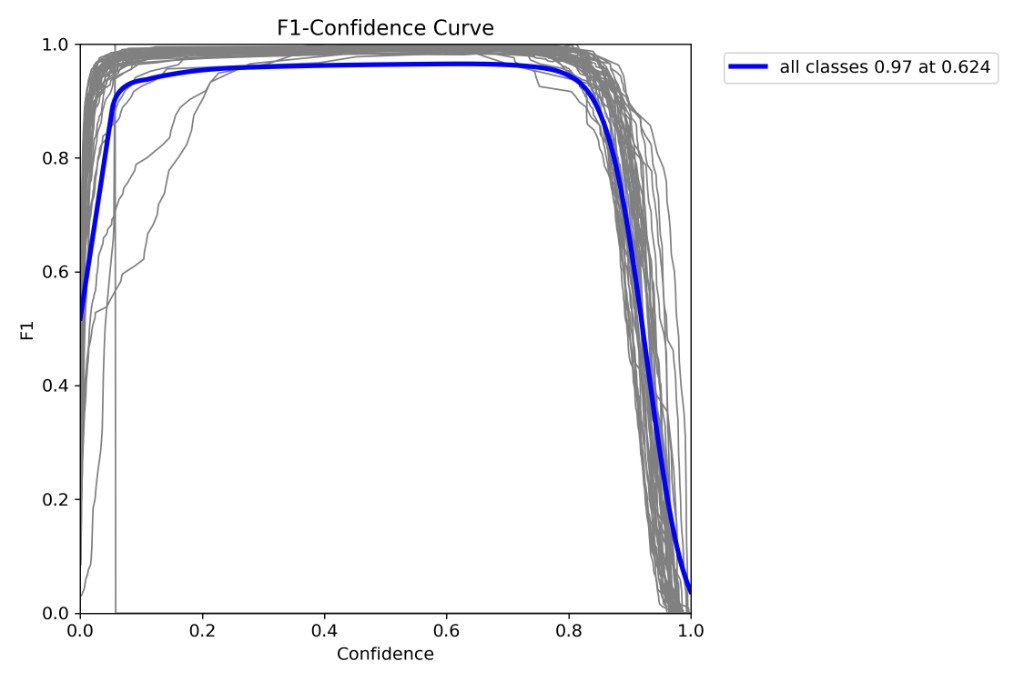
\includegraphics[width=\linewidth]{figures/lpr_char/ocr_boxF1_curve.png}
\caption{F1--confidence.}
\end{subfigure}
\caption{Ultralytics diagnostic curves for the 38-class character detector.}
\label{fig:ocrcurves}
\end{figure*}

\begin{figure*}[!tb]
\centering
\begin{subfigure}[b]{0.48\textwidth}\centering
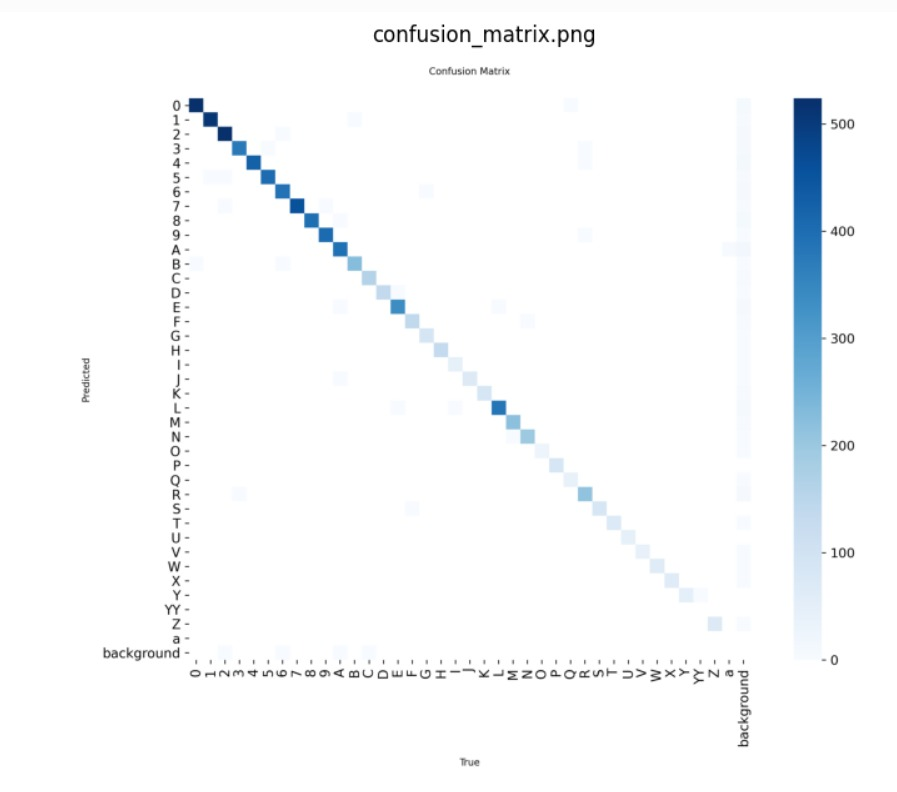
\includegraphics[width=\linewidth]{figures/lpr_char/ocr_confusion_matrix.png}
\caption{Counts confusion matrix.}
\end{subfigure}\hfil
\begin{subfigure}[b]{0.48\textwidth}\centering
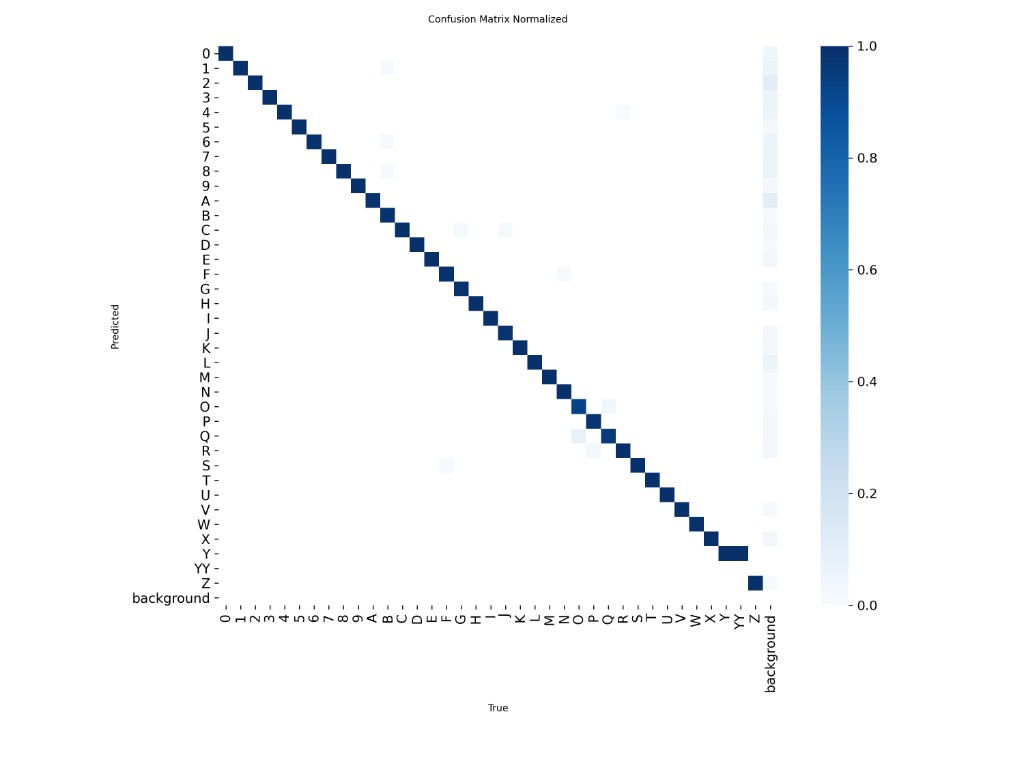
\includegraphics[width=\linewidth]{figures/lpr_char/ocr_confusion_normalized.png}
\caption{Normalized confusion matrix.}
\end{subfigure}
\caption{Confusion summaries across digits, letters, special tokens, and background.}
\label{fig:ocrconf}
\end{figure*}

\begin{figure*}[!tb]
\centering
\begin{subfigure}[b]{0.48\textwidth}\centering
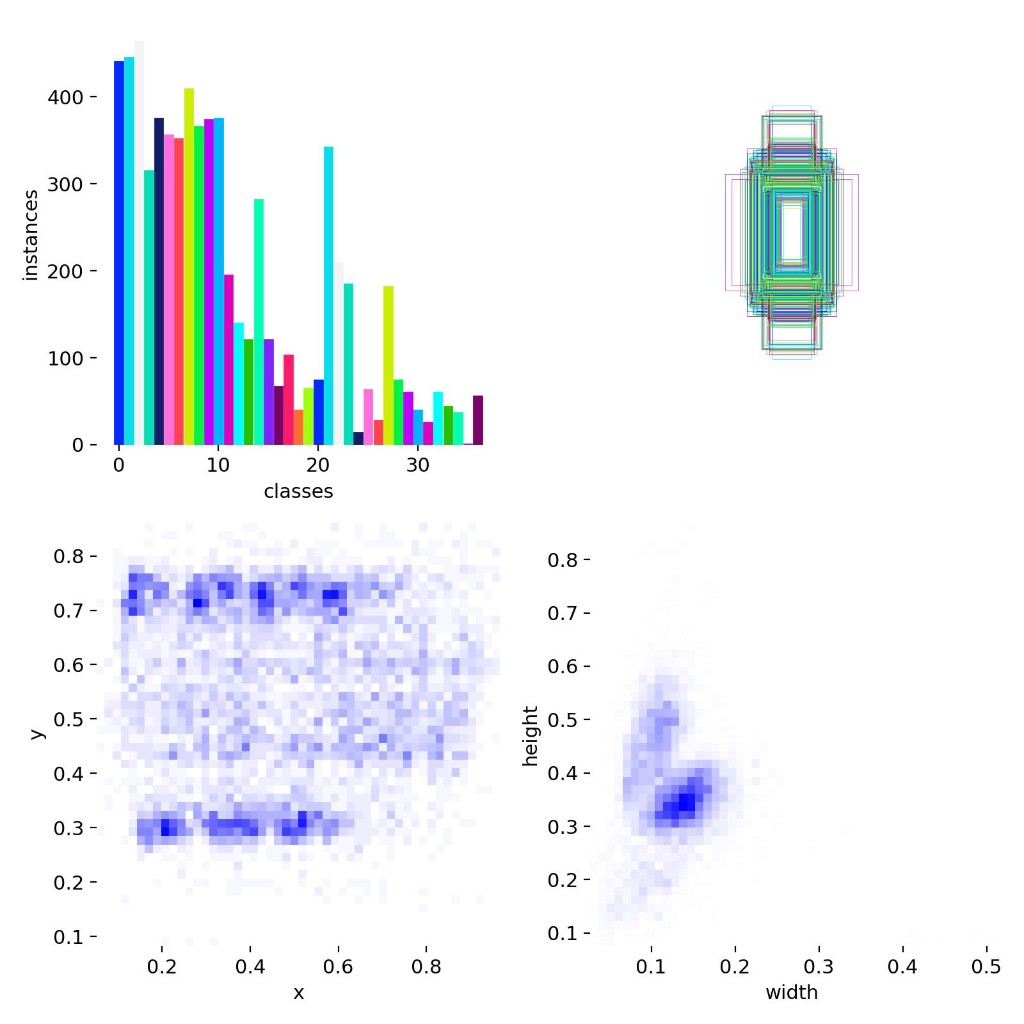
\includegraphics[width=\linewidth]{figures/lpr_char/ocr_labels.png}
\caption{Class histogram, box-shape overlay, and label center/size heatmaps.}
\end{subfigure}\hfil
\begin{subfigure}[b]{0.48\textwidth}\centering
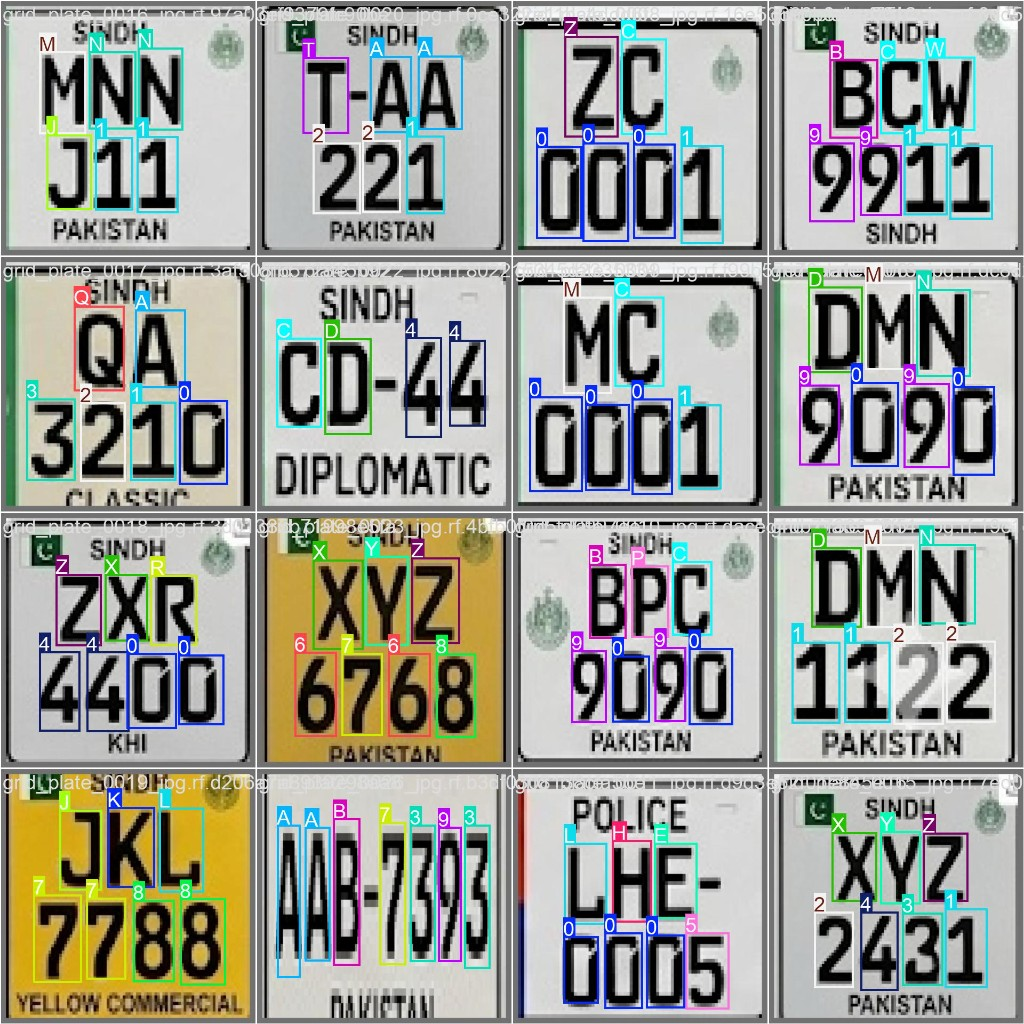
\includegraphics[width=\linewidth]{figures/lpr_char/ocr_val_batch_labels.png}
\caption{Validation batch mosaic with ground-truth character boxes.}
\end{subfigure}
\caption{Dataset analytics and batched validation tiles for the Roboflow v4 corpus.}
\label{fig:ocrlabelsval}
\end{figure*}

\begin{figure*}[!tb]
\centering
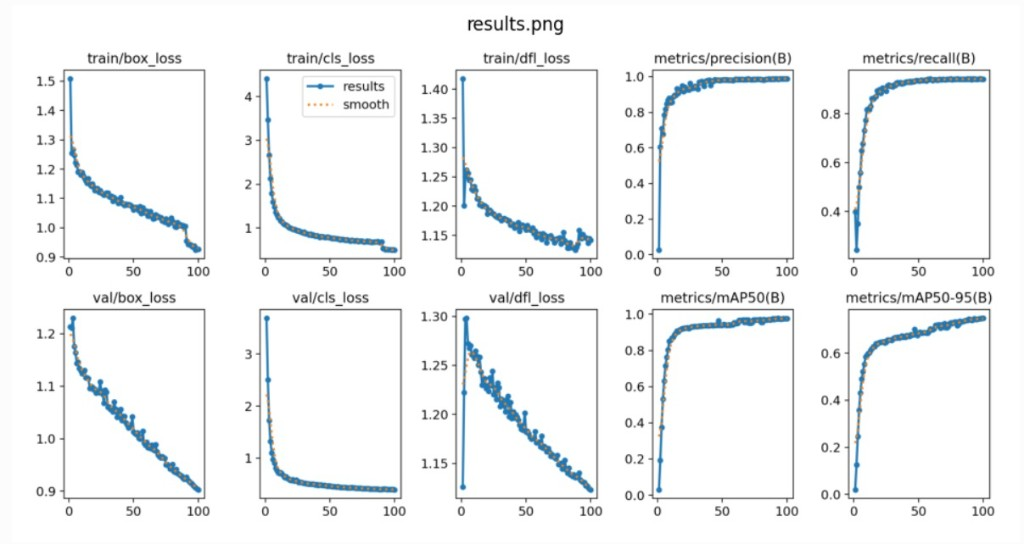
\includegraphics[width=\textwidth]{figures/lpr_char/ocr_training_results.png}
\caption{Training and validation losses plus box precision, recall, mAP@0.5, and mAP@0.5:0.95 over 100 epochs.}
\label{fig:ocrtrain}
\end{figure*}

\paragraph{VMMR (Vehicle Make \& Model) visual and diagnostic results.}\label{subsec:vmmrfigs}
Figures~\ref{fig:vmmrqual1}--\ref{fig:vmmrqual4} compile EfficientNet-B4 exports from the VMMR training run: test-metric summaries, partitioned confusion-matrix tiles, held-out inference overlays, training curves, and summary readouts. Figure~\ref{fig:vmmrconf245} shows the complete row-normalized 245-class confusion matrix on the held-out test split; the chunked tiles zoom selected class bands for readability.

\begin{figure*}[!tb]
\centering
\begin{subfigure}[b]{0.32\textwidth}\centering
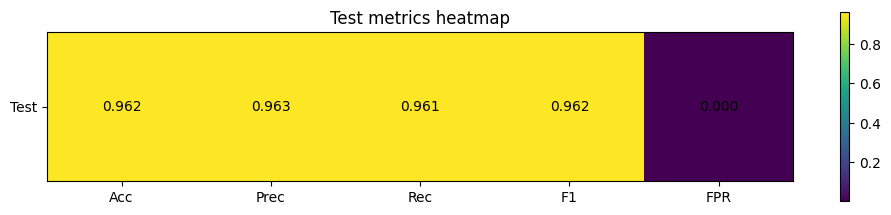
\includegraphics[width=\linewidth]{figures/vmmr/vmmr_01.png}
\caption{Test metrics heatmap (ACC, PREC, REC, F1, AUC).}
\end{subfigure}
\hfil
\begin{subfigure}[b]{0.32\textwidth}\centering
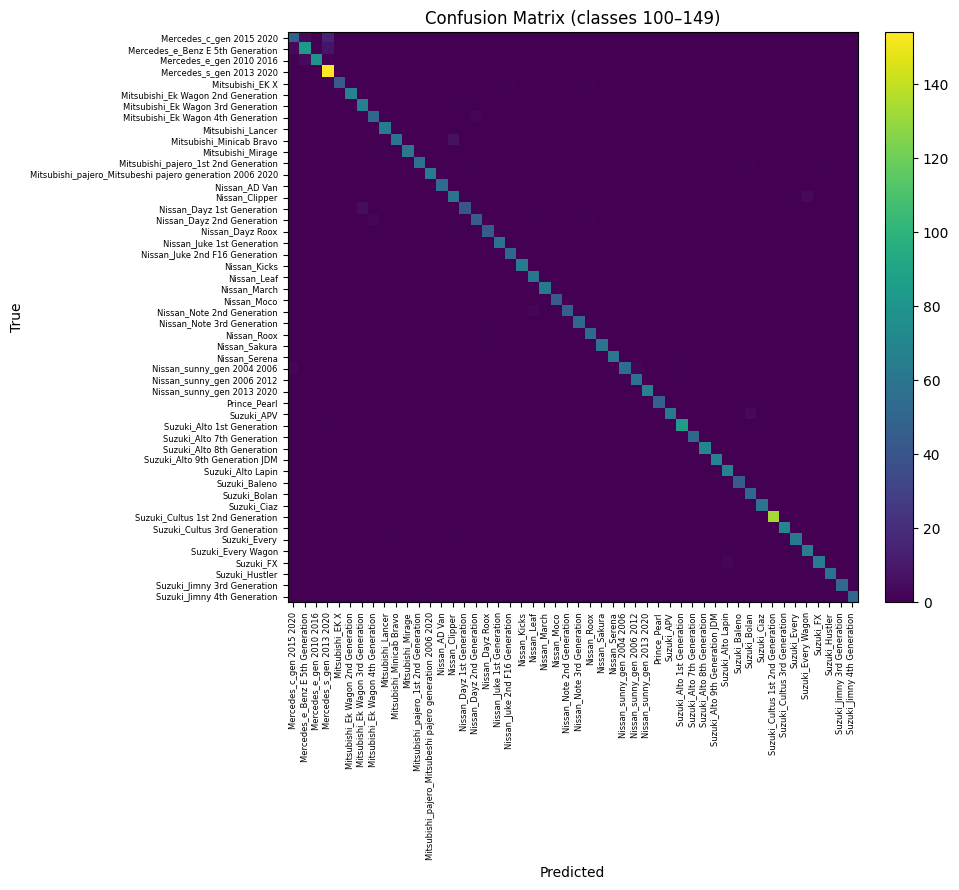
\includegraphics[width=\linewidth]{figures/vmmr/vmmr_02.png}
\caption{VMMR confusion matrix (classes 100--149).}
\end{subfigure}
\hfil
\begin{subfigure}[b]{0.32\textwidth}\centering
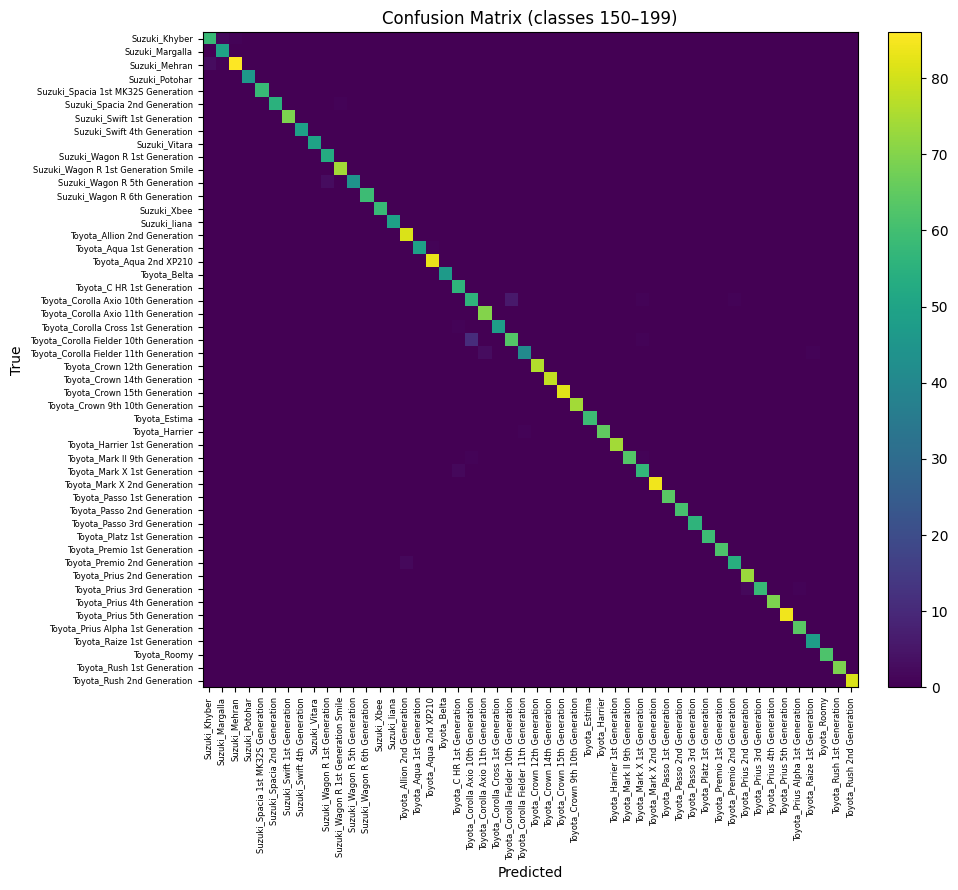
\includegraphics[width=\linewidth]{figures/vmmr/vmmr_03.png}
\caption{VMMR confusion matrix (classes 150--199).}
\end{subfigure}
\\[1.5ex]
\begin{subfigure}[b]{0.32\textwidth}\centering
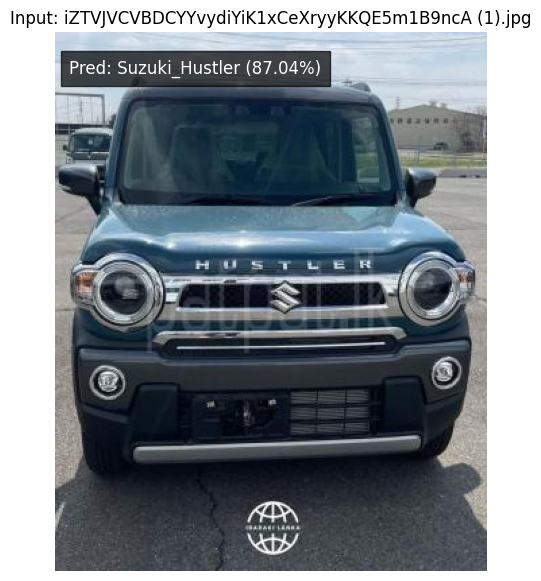
\includegraphics[width=\linewidth]{figures/vmmr/vmmr_04.png}
\caption{Suzuki Hustler inference overlay (87.04\%).}
\end{subfigure}
\hfil
\begin{subfigure}[b]{0.32\textwidth}\centering
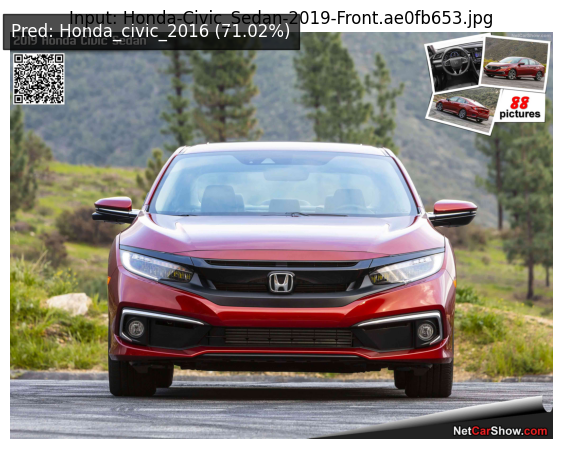
\includegraphics[width=\linewidth]{figures/vmmr/vmmr_05.png}
\caption{Honda Civic 2016 inference overlay (71.02\%).}
\end{subfigure}
\hfil
\begin{subfigure}[b]{0.32\textwidth}\centering
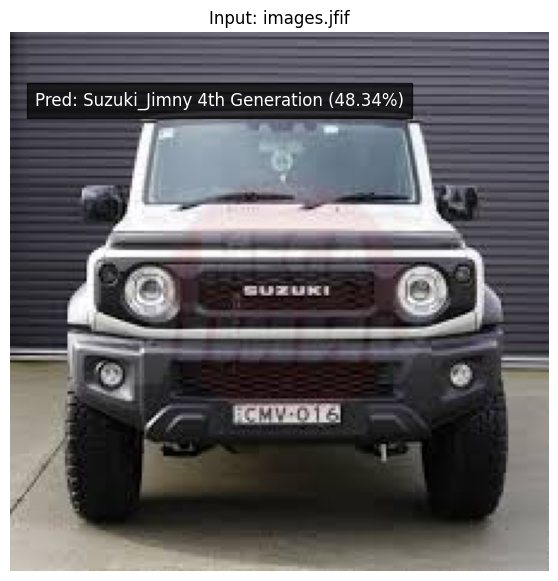
\includegraphics[width=\linewidth]{figures/vmmr/vmmr_06.png}
\caption{Suzuki Jimny 4th Gen inference overlay (48.34\%).}
\end{subfigure}
\\[1.5ex]
\begin{subfigure}[b]{0.32\textwidth}\centering
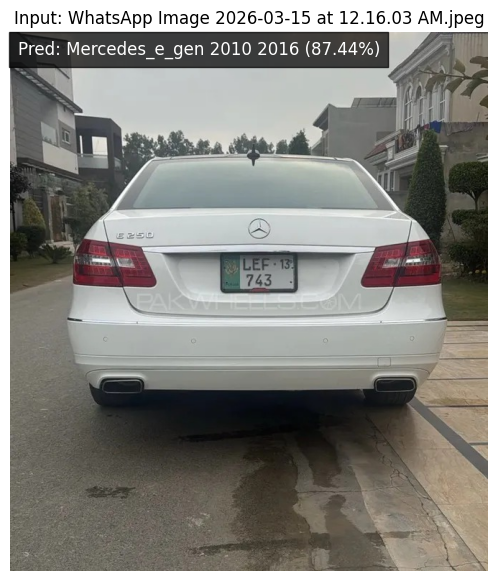
\includegraphics[width=\linewidth]{figures/vmmr/vmmr_07.png}
\caption{Mercedes E-Class sedan inference overlay (87.44\%).}
\end{subfigure}
\hfil
\begin{subfigure}[b]{0.32\textwidth}\centering
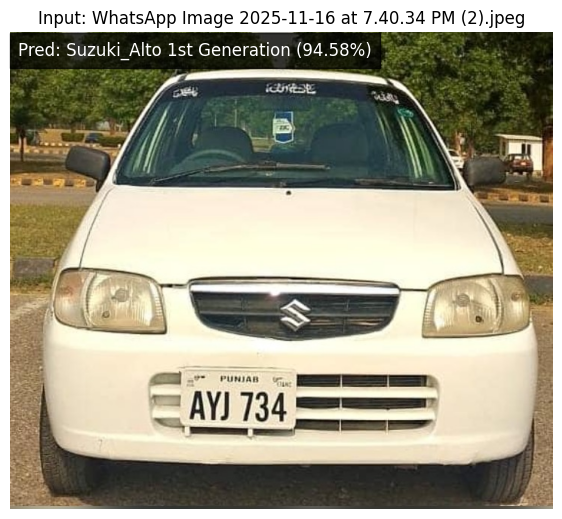
\includegraphics[width=\linewidth]{figures/vmmr/vmmr_08.png}
\caption{Suzuki Alto 1st Gen inference overlay (94.58\%).}
\end{subfigure}
\hfil
\begin{subfigure}[b]{0.32\textwidth}\centering
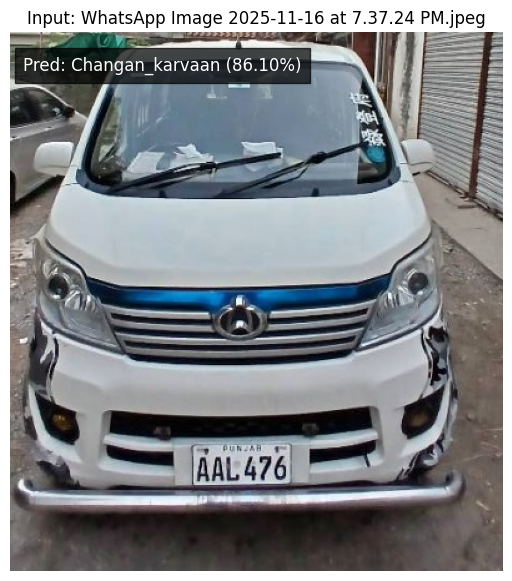
\includegraphics[width=\linewidth]{figures/vmmr/vmmr_09.png}
\caption{Changan Karvaan inference overlay (86.10\%).}
\end{subfigure}
\caption{EfficientNet-B4 VMMR gallery (batch 1/4): test-metric heatmap, confusion-matrix tiles, and held-out inference overlays with predicted make--model labels.}
\label{fig:vmmrqual1}
\end{figure*}

\begin{figure*}[!tb]
\centering
\begin{subfigure}[b]{0.32\textwidth}\centering
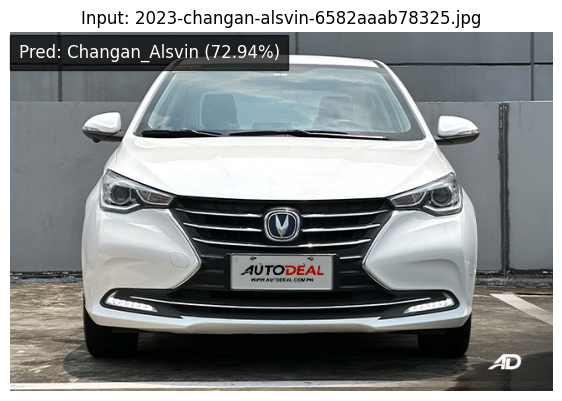
\includegraphics[width=\linewidth]{figures/vmmr/vmmr_10.png}
\caption{Changan Alsvin inference overlay (72.94\%).}
\end{subfigure}
\hfil
\begin{subfigure}[b]{0.32\textwidth}\centering
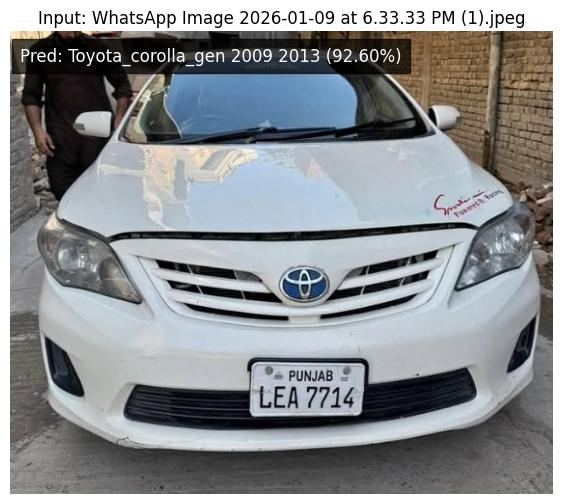
\includegraphics[width=\linewidth]{figures/vmmr/vmmr_11.png}
\caption{Toyota Corolla 2009--2013 inference overlay (92.60\%).}
\end{subfigure}
\hfil
\begin{subfigure}[b]{0.32\textwidth}\centering
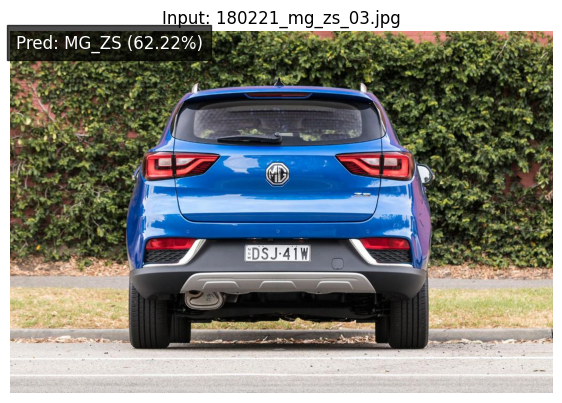
\includegraphics[width=\linewidth]{figures/vmmr/vmmr_12.png}
\caption{MG ZS SUV inference overlay (62.22\%).}
\end{subfigure}
\\[1.5ex]
\begin{subfigure}[b]{0.32\textwidth}\centering
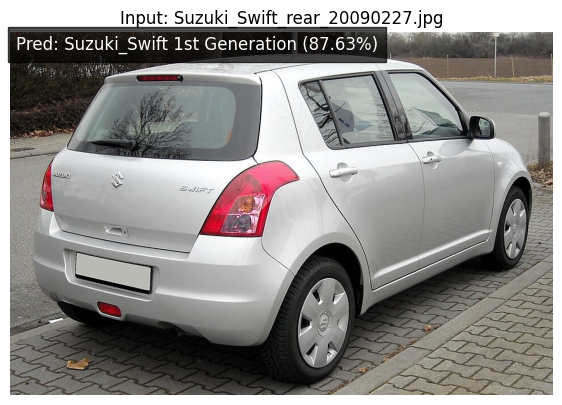
\includegraphics[width=\linewidth]{figures/vmmr/vmmr_13.png}
\caption{Suzuki Swift 1st Gen inference overlay (87.63\%).}
\end{subfigure}
\hfil
\begin{subfigure}[b]{0.32\textwidth}\centering
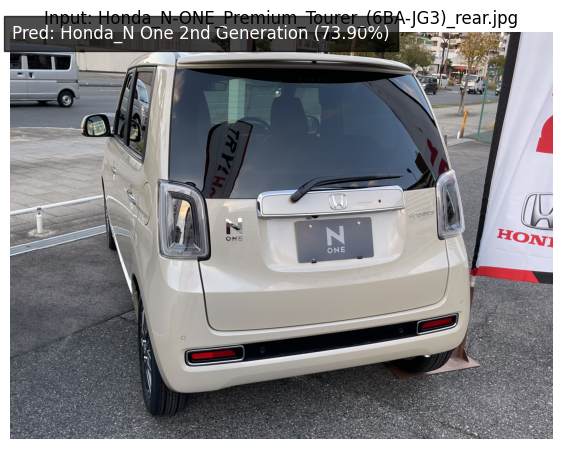
\includegraphics[width=\linewidth]{figures/vmmr/vmmr_14.png}
\caption{Honda N-One 2nd Gen inference overlay (73.90\%).}
\end{subfigure}
\hfil
\begin{subfigure}[b]{0.32\textwidth}\centering
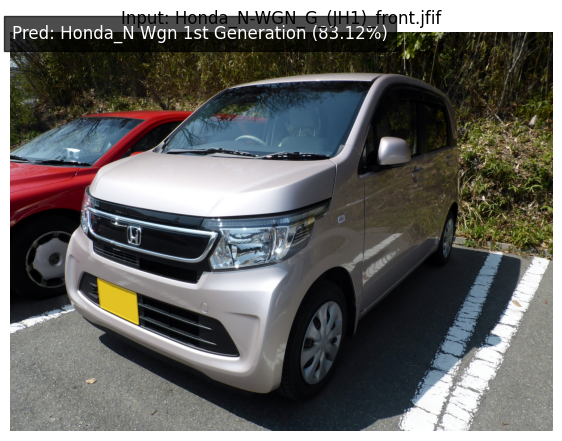
\includegraphics[width=\linewidth]{figures/vmmr/vmmr_15.png}
\caption{Honda N-Wgn 1st Gen inference overlay (83.12\%).}
\end{subfigure}
\\[1.5ex]
\begin{subfigure}[b]{0.32\textwidth}\centering
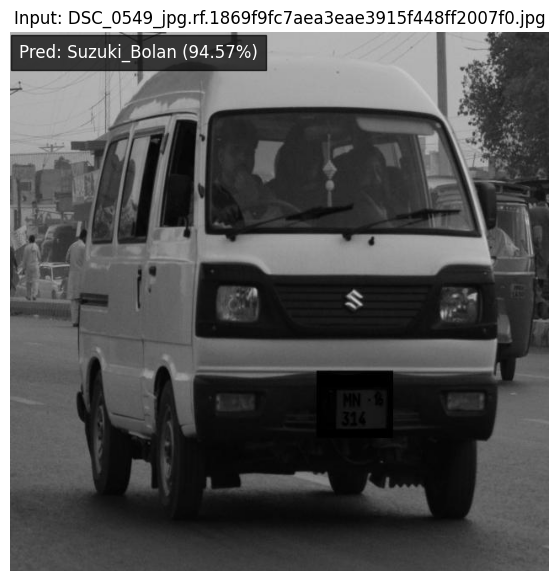
\includegraphics[width=\linewidth]{figures/vmmr/vmmr_16.png}
\caption{Suzuki Bolan inference overlay (94.57\%).}
\end{subfigure}
\hfil
\begin{subfigure}[b]{0.32\textwidth}\centering
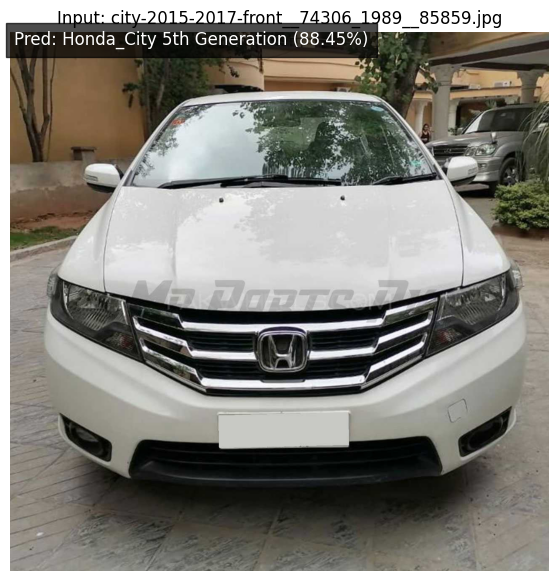
\includegraphics[width=\linewidth]{figures/vmmr/vmmr_17.png}
\caption{Honda City 5th Gen inference overlay (88.45\%).}
\end{subfigure}
\hfil
\begin{subfigure}[b]{0.32\textwidth}\centering
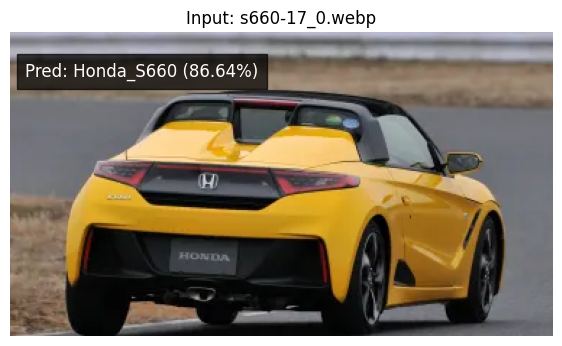
\includegraphics[width=\linewidth]{figures/vmmr/vmmr_18.png}
\caption{Honda S660 inference overlay (86.64\%).}
\end{subfigure}
\caption{EfficientNet-B4 held-out inference overlays (batch 2/4): each tile shows the input filename, predicted class, and confidence score.}
\label{fig:vmmrqual2}
\end{figure*}

\begin{figure*}[!tb]
\centering
\begin{subfigure}[b]{0.32\textwidth}\centering
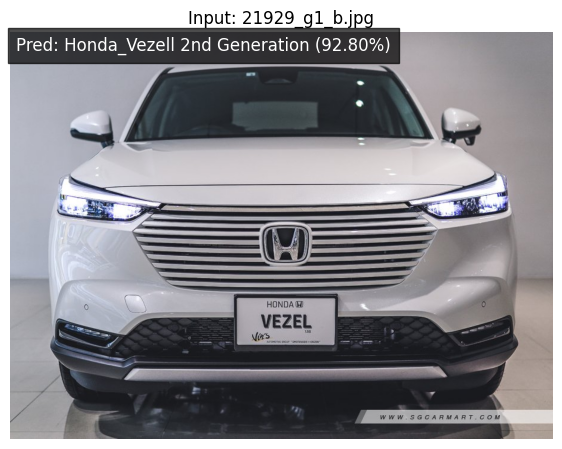
\includegraphics[width=\linewidth]{figures/vmmr/vmmr_19.png}
\caption{Honda Vezel 2nd Gen inference overlay (92.80\%).}
\end{subfigure}
\hfil
\begin{subfigure}[b]{0.32\textwidth}\centering
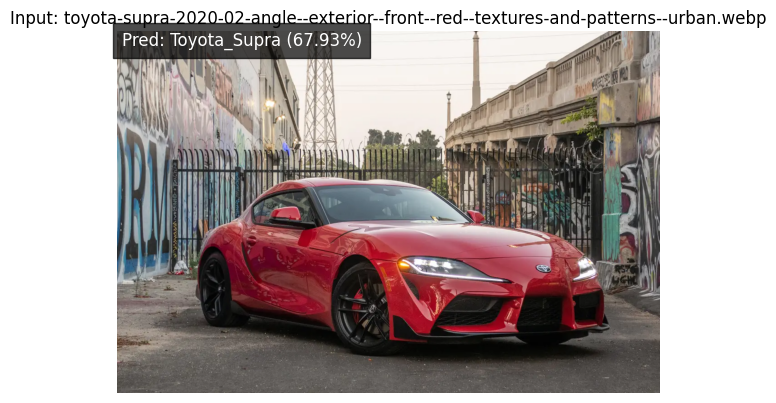
\includegraphics[width=\linewidth]{figures/vmmr/vmmr_20.png}
\caption{Toyota Supra inference overlay (67.93\%).}
\end{subfigure}
\hfil
\begin{subfigure}[b]{0.32\textwidth}\centering
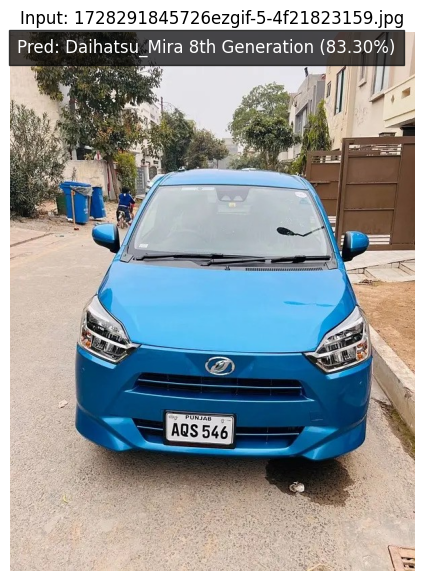
\includegraphics[width=\linewidth]{figures/vmmr/vmmr_21.png}
\caption{Daihatsu Mira 8th Gen inference overlay (83.30\%).}
\end{subfigure}
\\[1.5ex]
\begin{subfigure}[b]{0.32\textwidth}\centering
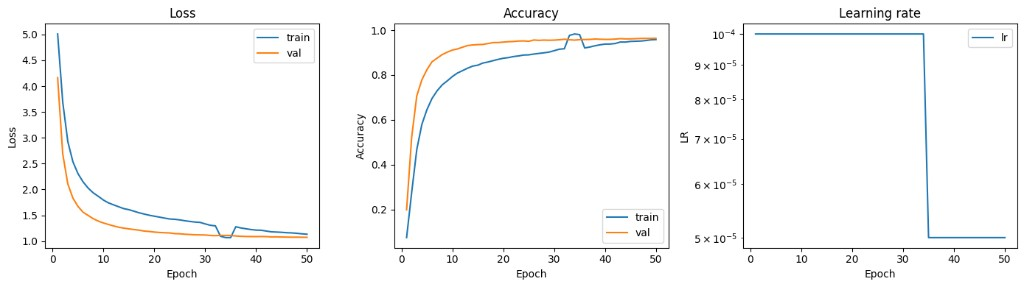
\includegraphics[width=\linewidth]{figures/vmmr/vmmr_22.png}
\caption{Training loss, accuracy, and learning-rate curves.}
\end{subfigure}
\hfil
\begin{subfigure}[b]{0.32\textwidth}\centering
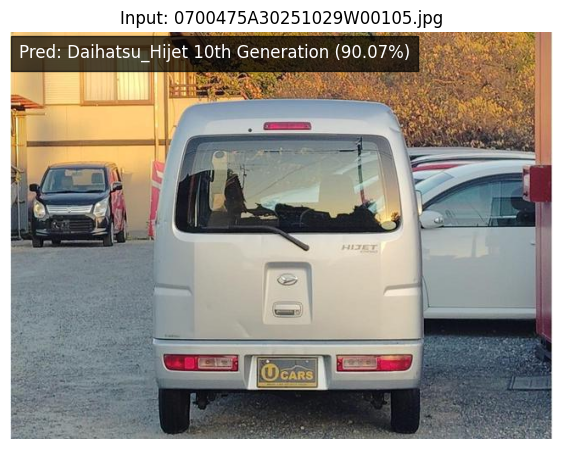
\includegraphics[width=\linewidth]{figures/vmmr/vmmr_23.png}
\caption{Daihatsu Hijet 10th Gen inference overlay (90.07\%).}
\end{subfigure}
\hfil
\begin{subfigure}[b]{0.32\textwidth}\centering
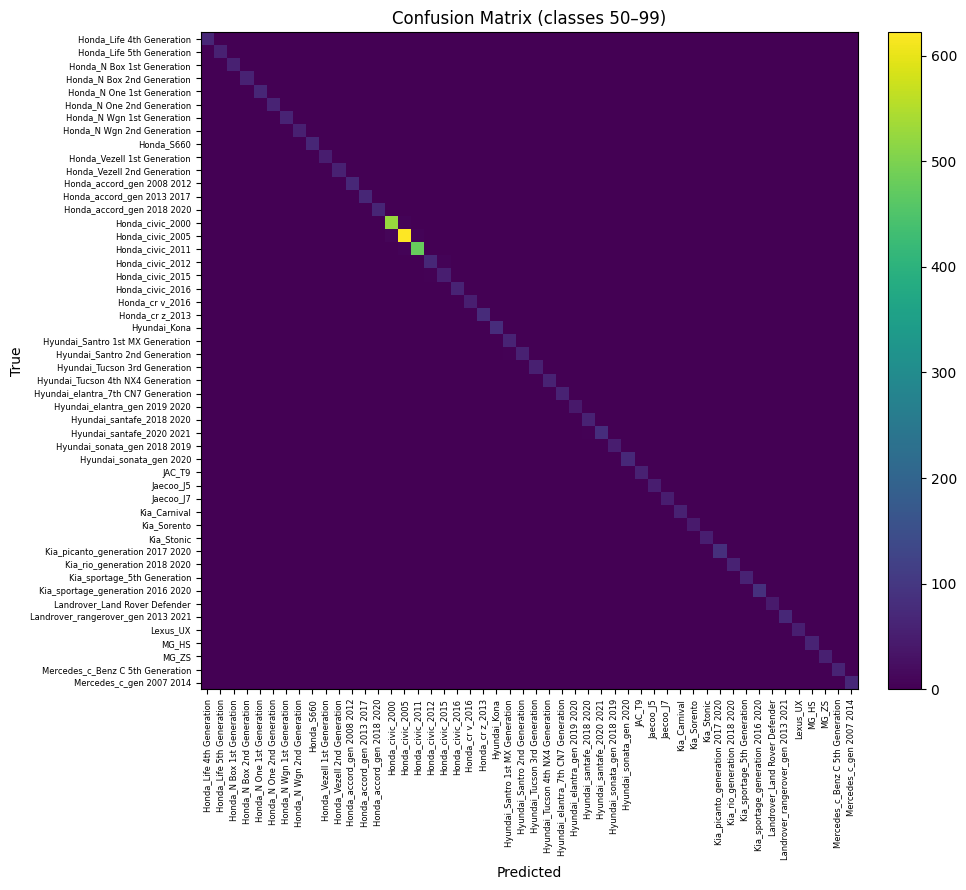
\includegraphics[width=\linewidth]{figures/vmmr/vmmr_24.png}
\caption{VMMR confusion matrix (classes 136--162).}
\end{subfigure}
\\[1.5ex]
\begin{subfigure}[b]{0.32\textwidth}\centering
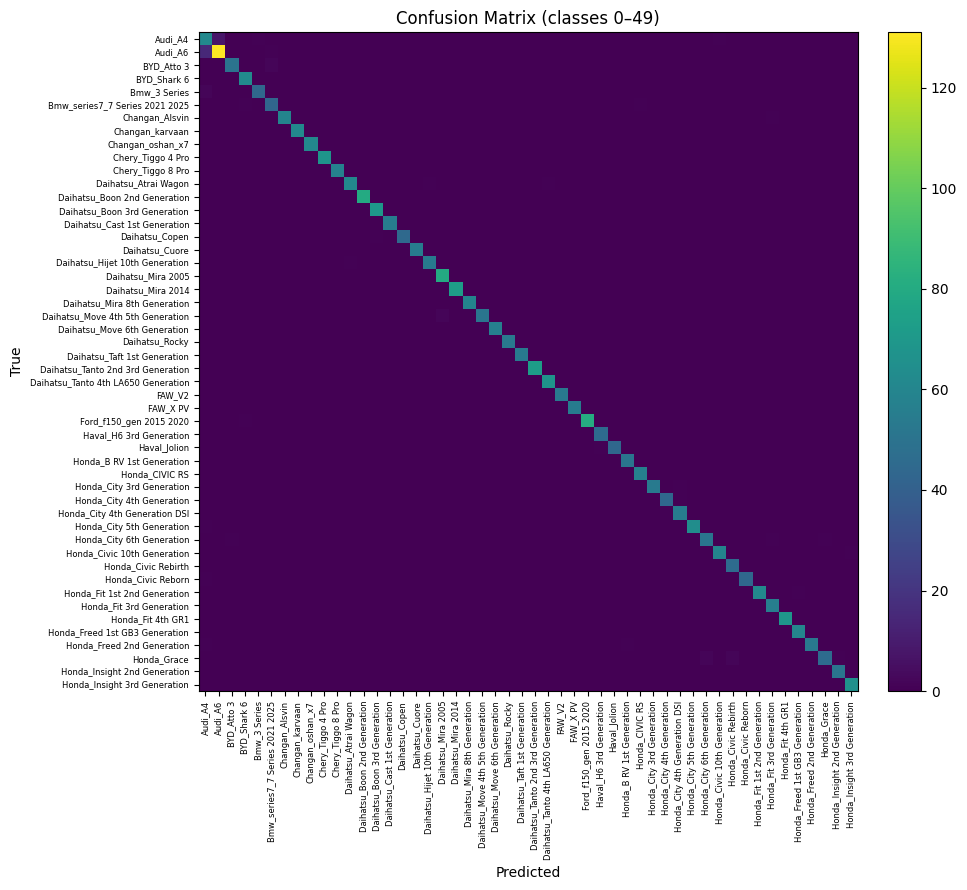
\includegraphics[width=\linewidth]{figures/vmmr/vmmr_25.png}
\caption{VMMR confusion matrix (classes 0--43).}
\end{subfigure}
\hfil
\begin{subfigure}[b]{0.32\textwidth}\centering
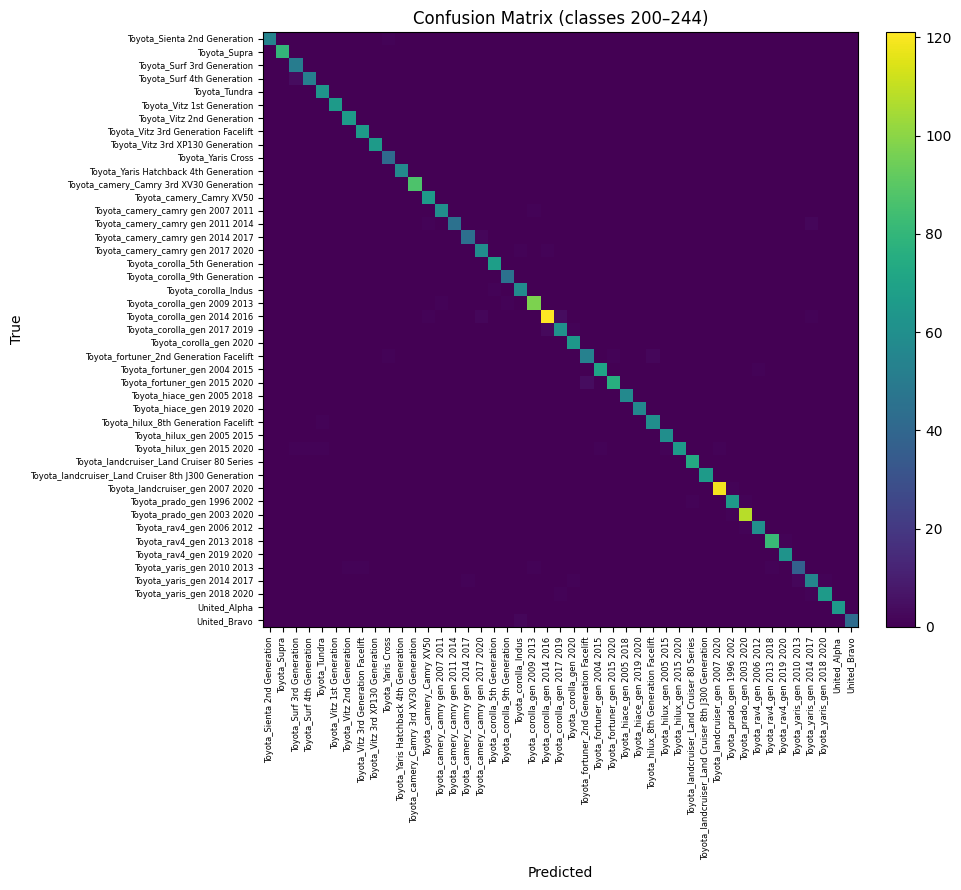
\includegraphics[width=\linewidth]{figures/vmmr/vmmr_26.png}
\caption{VMMR confusion matrix (classes 200--244).}
\end{subfigure}
\hfil
\begin{subfigure}[b]{0.32\textwidth}\centering
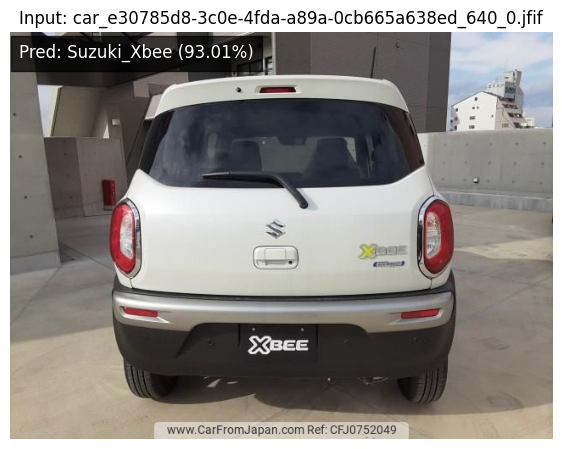
\includegraphics[width=\linewidth]{figures/vmmr/vmmr_27.png}
\caption{Suzuki Xbee inference overlay (93.01\%).}
\end{subfigure}
\caption{VMMR diagnostics mix (batch 3/4): inference overlays, epoch training curves, and partitioned confusion-matrix tiles.}
\label{fig:vmmrqual3}
\end{figure*}

\begin{figure*}[!tb]
\centering
\begin{subfigure}[b]{0.48\textwidth}\centering
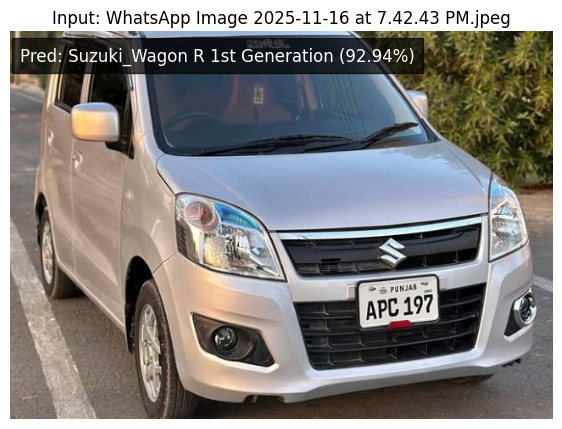
\includegraphics[width=\linewidth]{figures/vmmr/vmmr_28.png}
\caption{Top-5 prediction montage on held-out samples.}
\end{subfigure}
\hfil
\begin{subfigure}[b]{0.48\textwidth}\centering
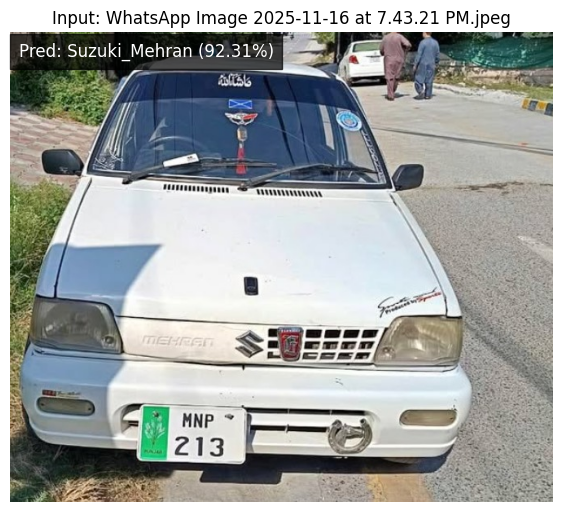
\includegraphics[width=\linewidth]{figures/vmmr/vmmr_29.png}
\caption{Macro false-positive-rate summary heatmap.}
\end{subfigure}
\\[1.5ex]
\begin{subfigure}[b]{0.48\textwidth}\centering
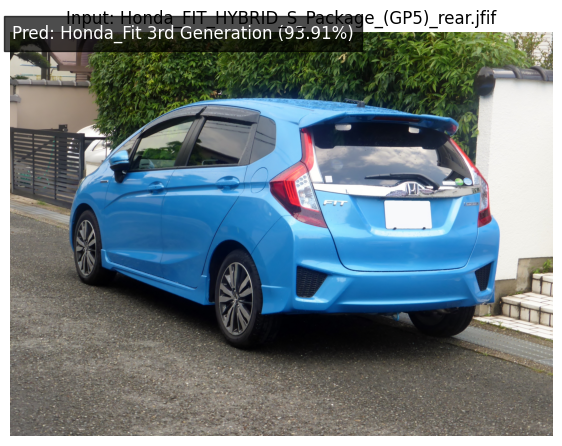
\includegraphics[width=\linewidth]{figures/vmmr/vmmr_30.png}
\caption{Per-class precision strip for tail classes.}
\end{subfigure}
\hfil
\begin{subfigure}[b]{0.48\textwidth}\centering
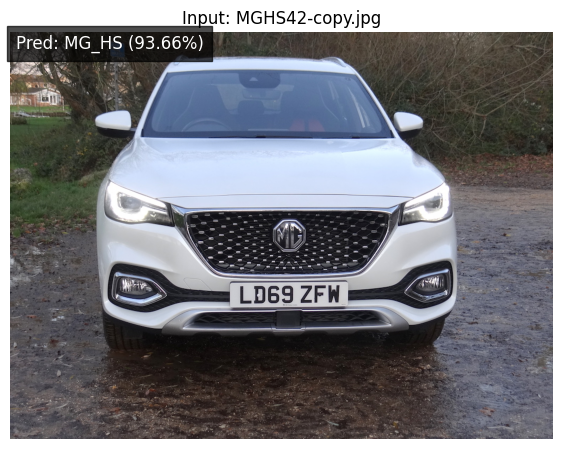
\includegraphics[width=\linewidth]{figures/vmmr/vmmr_31.png}
\caption{Printed aggregate test metrics (Top-1, macro-F1).}
\end{subfigure}
\caption{VMMR summary artifacts (batch 4/4): Top-5 montage, macro FPR, and aggregate test readouts.}
\label{fig:vmmrqual4}
\end{figure*}

\begin{figure*}[!tb]
\centering
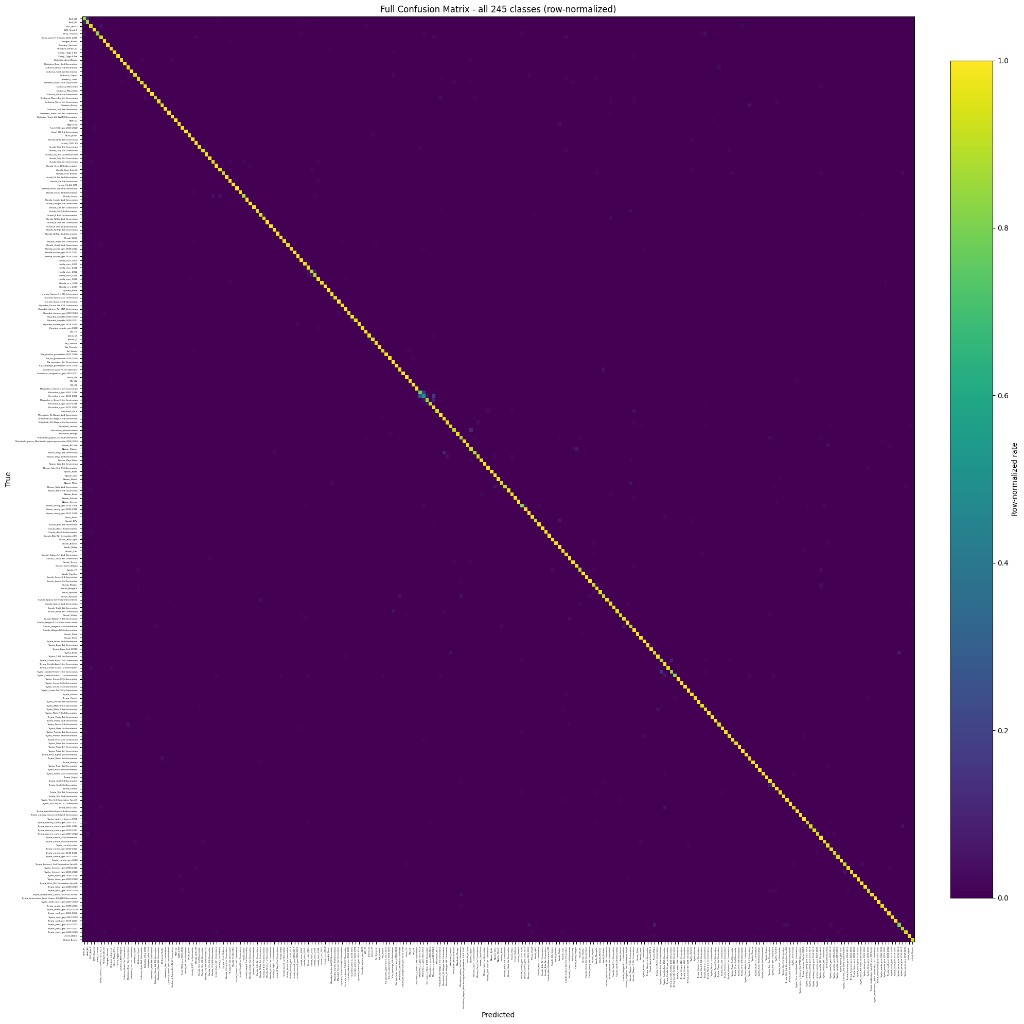
\includegraphics[width=0.78\textwidth]{figures/vmmr/vmmr_confusion_matrix_245.png}
\caption{Full row-normalized confusion matrix for all 245 VMMR classes on the held-out test split (EfficientNet-B4, epoch~50). Bright diagonal entries indicate correct make--model assignments; faint off-diagonal streaks mark occasional confusion between visually similar sibling-year classes.}
\label{fig:vmmrconf245}
\end{figure*}

\paragraph{Quantitative summaries and deployment notes.}
Tables~\ref{tab:lpdmetrics} and~\ref{tab:lpdtrain} hold LPD scores; Tables~\ref{tab:lpcharmetrics} and~\ref{tab:lpchartrain} hold character-stage scores with the mirroring caveat in Section~\ref{subsec:lpchar}. VMMR headline numbers sit in Section~\ref{sec:vmmr}. Table~\ref{tab:cmp} situates our prototype against representative cited systems. Edge latency on Orange Pi~5 Pro is reported in Subsection~\ref{subsec:hwdeploy} (Figure~\ref{fig:hw_latency}); end-to-end string accuracy per weather branch and per-condition VMMR rescoring remain future work. The next paragraphs explain how to read IoU/mAP and the confusion-matrix tiles without drowning in symbols.

\par\vspace{2pt}\noindent\footnotesize\textit{Validation caveat (character stage):} Character mAP@0.5 in Table~\ref{tab:lpcharmetrics} and the Char column of Table~\ref{tab:cmp} were computed with validation images mirrored from training (Section~\ref{subsec:lpchar}). Treat these as upper-bound diagnostics, not held-out generalization. LPD and VMMR metrics use standard disjoint splits.\par\vspace{4pt}

\begin{table*}[!htbp]
\centering
\caption{Comparison with representative systems. Competitor figures are approximate summaries from cited works ($^\ast$); our character mAP@0.5 uses mirrored validation ($^\dagger$); VMMR Top-1 is at $224^2$ test resolution ($^\ddagger$).}
\label{tab:cmp}
\begin{tabular}{@{}lccccc@{}}
\toprule
System & LPD mAP@0.5 & Char mAP@0.5 & VMMR Top-1 & Weather & Dual \\
\midrule
Thapliyal et al.~\cite{r01} & $\sim$0.94$^\ast$ & --- & --- & Clear-biased & No \\
Plavac et al.~\cite{r05} & $\sim$0.78$^\ast$ & --- & --- & Field rain/fog & No \\
Intertraff~\cite{r10} & --- & --- & --- & Adverse focus & No \\
FYP prototype & 0.9807 & 0.977$^\dagger$ & 0.9624$^\ddagger$ & Fog/Rain hooks & Yes \\
\bottomrule
\end{tabular}
\end{table*}

% --- Metrics, detection theory, and confusion-matrix interpretation ---
\paragraph{Intersection-over-Union and localization quality.}
For axis-aligned boxes $b^{\mathrm{gt}}$ and $b^{\mathrm{pred}}$, $\mathrm{IoU} = \mathrm{area}(b^{\mathrm{gt}} \cap b^{\mathrm{pred}}) / \mathrm{area}(b^{\mathrm{gt}} \cup b^{\mathrm{pred}})$. mAP averages precision across IoU sweeps; mAP@0.5 is the headline we cite for gate-distance plates. Table~\ref{tab:lpdmetrics} is epoch~50 LPD; Table~\ref{tab:lpcharmetrics} is epoch~100 over 38 classes with the training-mirror caveat (Section~\ref{subsec:lpchar}). Qualitative tiles nearby show what those numbers feel like.

\paragraph{Non-maximum suppression and duplicate detections.}
NMS deletes duplicate boxes once IoU crosses the default Ultralytics threshold. Fancy plate frames sometimes fire twice; log NMS and confidence (0.25 in our integrated path) whenever you share a new export.

\paragraph{Confusion matrix structure for 245 classes.}
Let $C \in \mathbb{N}^{K\times K}$ be the confusion matrix with rows as ground truth and columns as predictions. Diagonal mass concentrates on easy classes; off-diagonal streaks along visually similar siblings (adjacent model years) motivate hierarchical evaluation (make-level aggregation) in future reports. The full 245-way matrix appears in Figure~\ref{fig:vmmrconf245}; chunked zoom tiles appear in Figures~\ref{fig:vmmrqual1}--\ref{fig:vmmrqual3}.

\paragraph{Calibration and expected calibration error.}
Accurate models can still be overconfident. A quick temperature fit on validation logits would lower ECE before we trust softmax thresholds for \textsc{alert}.

\paragraph{Label smoothing and decision margins.}
Label smoothing $\epsilon$ in~\eqref{eq:labelsmooth} shrinks logits toward uniformity, widening margins against overconfident mistakes. Training used $\epsilon{=}0.1$ in cross-entropy, which interacts with macro-FPR estimates on the test split.

\paragraph{Reproducibility checklist.}
Pin seeds, GPU name, dataset SHA, and package versions when publishing. This draft copies numbers straight from the training logs; a frozen dependency manifest is still on the to-do list.

\paragraph{Hardware deployment notes.}
Field deployment uses the stack in Figure~\ref{fig:hw} and Subsection~\ref{subsec:hwdeploy}: Orange Pi~5 Pro (16\,GB), USB 1080p camera, 5\,V/5\,A supply, and HDMI preview. The edge package achieves 700--1000\,ms per frame (Figure~\ref{fig:hw_latency}) while posting annotated events to the Vercel dashboard (Figure~\ref{fig:hw_dashboard}). Relay-driven gate motors, IR fill lighting, outdoor enclosure, and pole-mounted sensors remain target extensions per Table~\ref{tab:hw}; GPIO/LED indicators are optional on the deployed board.

\section{Discussion}
\label{sec:disc}
\subsection{Preprocessing Effectiveness}
Defogging lifts local contrast so YOLO sees plate edges again: dark-channel transmission in~\eqref{eq:scatter} followed by LAB CLAHE (Section~\ref{sec:pre}) recovers mid-tone structure that flat haze otherwise washes out. Field evaluations of commercial ALPR under rain and fog report sizable recall drops relative to clear-day marketing demos~\cite{r05,r10}; our preprocessing targets that gap without claiming a learned derainer. Rain filtering remains a balancing act---stacked vertical medians suppress streak energy, yet aggressive filtering can melt character strokes, which motivated edge-aware masks around the plate band. Qualitative overlays in Figures~\ref{fig:prepipefog}--\ref{fig:prepiperain} show readable plate boxes after mitigation, but we have not yet tabulated string-level accuracy per branch; that controlled study is future work.

\subsection{LPR Analysis}
Our LPD mAP@0.5 of 0.9807 on Roboflow v1 (Table~\ref{tab:lpdmetrics}) exceeds approximate YOLOv5 ALPR localization figures reported near 0.94 in related single-dataset studies~\cite{r01}, while remaining on par with strong detector-first pipelines~\cite{r06}. High plate mAP mostly certifies rectangle localization, not full-string reading. Character mAP@0.5 of 0.977 (Figure~\ref{fig:ocrmetrics}, Table~\ref{tab:lpcharmetrics}) looks competitive with thesis comparisons to $\sim$93\% end-to-end ANPR systems that lean on EasyOCR~\cite{r03}, yet our character validation mirrored training (Section~\ref{subsec:lpchar}), so we expect a measurable drop once a disjoint Roboflow validation split is used---the validation caveat before Table~\ref{tab:cmp} flags this explicitly. Motion blur and O/0-style ambiguities remain; temporal voting across 3--5 frames at 15\,fps would add only $\sim$200\,ms latency while filtering sporadic misreads.

\subsection{VMMR Analysis}
EfficientNet-B4 at 0.9624 Top-1 and 0.9618 macro-F1 on 17{,}254 held-out test images compares favorably with unified ANPR+VMMR reports near 90.6\% on smaller Pakistani corpora~\cite{r03} and fine-grained gate-security work emphasizing attention over breadth~\cite{r08}. Macro FPR of 0.0002 looks encouraging but can understate pain on visually similar sibling years (Figures~\ref{fig:vmmrconf245} and~\ref{fig:vmmrqual3}--\ref{fig:vmmrqual4}). The $224^2$ versus $380^2$ deploy skew (Section~\ref{sec:vmmr}) means integrated demo overlays should not be read as replicating the 0.9624 benchmark; fine-grained classifiers are sensitive to resolution shift, and unifying input size is a prerequisite for field claims.

\subsection{Dual Verification Security}
Plate-only gates fail when a copied plate is mounted on the wrong vehicle. Comparing read string $s$ with predicted make/model $y$ blocks casual spoofing: a sedan plate on an SUV triggers \textsc{alert} under our policy (Section~\ref{sec:gate}). This is weaker than biometrics or RFID, yet stronger than whitelist-only ANPR kits surveyed in commercial white papers~\cite{r09,r29}. Quantitatively, if plate reading alone mis-associates 2--5\% of visits under blur and cloned plates occur in even a fraction of abuse attempts, dual verification converts a silent \textsc{grant} into a human-review event---trading a modest latency and policy-complexity cost for auditability.

\subsection{Limitations}
We lack snowy data, disjoint character validation, automatic weather routing, and physical relay actuation on a lane motor. LPD diagnostic plots use $640^2$ exports while training used $384^2$. End-to-end string accuracy under each weather branch and VMMR rescoring after fog/rain injection are not yet benchmarked. These are engineering follow-ups with clear protocols rather than conceptual blockers.


\section{Conclusion and Future Work}
\label{sec:conc}
\subsection{Conclusion}
This FYP built a defog/de-rain front end, a two-head YOLOv8n LPR stack, and an EfficientNet-B4 VMMR classifier, then glued them together with a dual-check policy in a web demo. On Roboflow \emph{License Plate Project} v1, YOLOv8n LPD reached precision 0.9850, recall 0.9553, mAP@0.5 0.9807, and mAP@0.5:0.95 0.7073 at epoch~50 on a standard disjoint validation split. EfficientNet-B4 achieved 0.9624 Top-1 accuracy on 17{,}254 test photos at $224^2$ (Top-5 $=0.9939$) with macro precision/recall/F1 of 0.9634/0.9612/0.9618. The 38-class head reported mAP@0.5 0.977, precision 0.990, recall 0.942, F1 0.965, and FPR 0.010 at epoch~100 (Figure~\ref{fig:ocrmetrics}), with mAP@0.5:0.95 0.7611 in the Ultralytics export, but validation images were mirrored from training (Section~\ref{subsec:lpchar}); readers should \emph{not} treat that character mAP as a held-out generalization figure alongside the LPD and VMMR test metrics.

\subsection{Future Work}
Short term: align all modules to one inference resolution ($224^2$ or $384^2$), export TensorRT/OpenVINO builds for Orange Pi~5, add temporal voting, and complete string-level LPR benchmarks under fog/rain/night branches with ground-truth transcripts. Medium term: collect snow/smog sets, add sensors for automatic branch selection, obtain a real Roboflow validation split for characters, temperature-calibrate softmax scores before policy thresholds, and wire relay timing on a field-mounted gate motor. Longer term ideas---federated updates, richer audit dashboards, visitor mobile apps---follow once the lane stack is fully outdoor-hardened.

\section*{Acknowledgment}
We thank our supervisor, Dr.~Taimoor Naeem (Department of Computer Engineering, COMSATS University Islamabad, Lahore Campus), for guidance throughout the project and for tolerating last-minute experiment reruns.

\appendices

\section{Supplementary Mathematical Notes}
\label{app:math}
We collected the formulas examiners asked about in the defense: Koschmieder visibility, dark-channel algebra, why LAB CLAHE beats RGB CLAHE, median streak intuition, Telea's local update, label smoothing, and macro vs.\ micro metrics. None of this is new theory; it is scratch paper turned printable.

\subsection{Koschmieder Visibility and Airlight}
Under homogeneous attenuation with extinction coefficient $\beta$, the apparent radiance of a distant object obeys $L(d)=L_\infty (1-e^{-\beta d}) + A e^{-\beta d}$, where $A$ is airlight and $L_\infty$ is the intrinsic object radiance. Visibility $V$ is often defined as the distance at which contrast drops below a threshold, yielding an approximate inverse relationship between $V$ and $\beta$. Dark-channel dehazing estimates a pixel-wise transmission $t(x)$ related to relative depth and $\beta$ along lines of sight.

\subsection{Dark-Channel Algebraic Steps}
Given color channels $I_c$ for $c\in\{R,G,B\}$, the dark channel is $I_{\mathrm{dark}}(x)=\min_c \min_{y\in\Omega(x)} I_c(y)$ with local patch $\Omega$. Atmospheric light $A$ is estimated from the brightest intensities in the top fraction of darkest locations. A coarse transmission follows $t(x)=1-\omega\, I_{\mathrm{dark}}(x)/A$ with $\omega\in(0,1]$ to retain a small amount of haze for naturalness. Our code then refines $t$ with guided filtering on a grayscale guide so edges stay aligned.

\subsection{LAB Color Space Jacobian Intuition}
Let $(L,a,b)$ denote LAB channels. Small perturbations in $L$ primarily affect luminance perception, while $a,b$ encode opponent chromatic axes. Applying CLAHE only on $L$ reduces cross-channel bleeding relative to applying histogram equalization independently on RGB channels, which can distort perceived hue.

\subsection{Gamma Curve Curvature}
The second derivative of $g(u)=u^{1/\gamma}$ with respect to $u\in[0,1]$ is $g''(u)=\tfrac{1}{\gamma}(\tfrac{1}{\gamma}-1)u^{1/\gamma-2}$. For $\gamma<1$, the curve is convex-up in log-log coordinates, boosting mid-tones; for $\gamma>1$, mid-tones compress. The fog pipeline clips $\gamma$ to $[0.6,1.8]$ after computing a data-driven exponent from mean gray.

\subsection{Vertical Median as Minimax under Impulse Noise}
Median filtering minimizes the $\ell_1$ loss to a constant predictor within each window under salt-and-pepper noise models; oriented median stacks approximate streak suppression when streak directions align with the filtering axis.

\subsection{Telea Inpainting Local Formulation (Sketch)}
Telea's fast marching method propagates known boundary values along normals into unknown regions by combining isophote direction and gradient strength; the OpenCV implementation exposes a radius parameter (set to 3 in the rain spot inpainting stage) controlling locality of the fill.

\subsection{Softmax and Cross-Entropy with Label Smoothing}
Let logits be $z\in\mathbb{R}^K$, softmax $p_i=e^{z_i}/\sum_j e^{z_j}$, and smoothed targets $q_i=(1-\epsilon)\,\mathbf{1}[i=y]+\epsilon/K$. The cross-entropy $-\sum_i q_i\log p_i$ penalizes overconfident spikes when $\epsilon>0$, improving generalization in many large-scale classifiers.

\subsection{Macro versus Micro Averaging}
Micro-averaged metrics aggregate counts globally and can be dominated by head classes. Macro averages compute per-class metrics and average with equal weight, which better reflects tail behavior in fine-grained VMMR with 245 classes.

\subsection{Compound Scaling Constraint Recap}
EfficientNet chooses $\alpha,\beta,\gamma$ and searches a baseline depth multiplier $\phi$ such that memory and FLOP budgets are respected. B4 represents a middle-high capacity point favorable when GPU memory exceeds mobile phones but remains bounded on Colab GPUs.

\subsection{Two-Stage YOLO Information Flow}
Let $f_{\mathrm{plate}}$ produce boxes $B=\{b_m\}$; in this project $f_{\mathrm{plate}}$ is the YOLOv8n LPD trained on Roboflow v1 with validation mAP@0.5 reported in Table~\ref{tab:lpdmetrics}. For each crop $I|_{b_m}$, $f_{\mathrm{char}}$ is the YOLOv8n 38-class detector trained on Roboflow \emph{My First Project} version~4 with aggregate box metrics in Table~\ref{tab:lpcharmetrics}. It predicts character boxes $\{c_n\}$ with classes. Reading order sorts centers along $x$, yielding a sequence decoded by the formatter. Error modes include missed $B$ (false negative localization), merged characters (low NMS threshold), and swapped digits/letters under motion blur.

\subsection{Expected Calibration Error Definition}
Partition predicted probabilities into bins $\{B_m\}$; ECE is $\sum_m \frac{|B_m|}{N}\,|\mathrm{acc}(B_m)-\mathrm{conf}(B_m)|$. Lower ECE indicates better alignment between stated confidence and empirical correctness.

\paragraph{Summary.} Think of this appendix as the cheat sheet linking physics (fog, rain) to the code knobs we touched.

\section{Hardware Specifications}
\label{app:hw}
This appendix mirrors thesis Appendix~C. Pin numbers below use BCM notation for Orange Pi~5; verify polarity against the relay module datasheet before energizing coils. Mains wiring belongs to a licensed electrician; students should only ever touch 3.3\,V logic.

{\footnotesize
\setlength{\tabcolsep}{3pt}
\renewcommand{\arraystretch}{1.05}
\begin{table}[!htbp]
\centering
\caption{Target lane bill of materials (status: software validated on GPU; hardware integration planned).}
\label{tab:hwapp}
\begin{tabular}{@{}p{0.22\columnwidth}p{0.34\columnwidth}p{0.36\columnwidth}@{}}
\toprule
Component & Specification & Role \\
\midrule
Lane camera & IR-sensitive imager + 850\,nm LED fill & Night/haze plate visibility \\
Edge computer & Orange Pi~5, 8\,GB RAM & On-device inference and GPIO \\
Relay module & Opto-isolated, flyback-protected & Isolate Pi from motor driver \\
Motor controller & Commercial gate drive (Centsys-class) & Barrier open/close commands \\
Power supply & Outdoor-rated 12/24\,V PSU with fuse & Camera, Pi, relay, sensors \\
Enclosure & IP65 cabinet with cable glands & Weather protection for electronics \\
Cabling & PoE or separate Ethernet + power runs & Lane connectivity \\
\bottomrule
\end{tabular}
\end{table}

\begin{table}[!htbp]
\centering
\caption{Planned interface signals (BCM numbering for Orange Pi~5; verify against module datasheets).}
\begin{tabular}{@{}p{0.24\columnwidth}p{0.18\columnwidth}p{0.50\columnwidth}@{}}
\toprule
Signal & Pin (BCM) & Notes \\
\midrule
Relay channel 1 (grant) & TBD & Active-high or low per module; flyback diode on coil \\
Relay GND & GND & Common return \\
Optional sensor I$^2$C & GPIO\,2/3 (SDA/SCL) & Weather / lux boards (future) \\
Status LED & TBD & Optional lane feedback \\
\bottomrule
\end{tabular}
\end{table}
}

\section{Dataset Samples}
Supplementary tiles should come from the held-out test split where possible so readers see unseen vehicles, not only training favorites.

\clearpage
\balance
\nocite{r01,r02,r03,r04,r05,r06,r07,r08,r09,r10,r11,r12,r13,r14,r15,r16,r17,r18,r19,r20,r21,r22,r23,r24,r25,r26,r27,r28,r29,r30,r31,r32,r33,r34,r35,r36,r37,r38,r39,r40,r41,r42}
\bibliographystyle{IEEEtran}
\bibliography{references}

\end{document}
